\documentclass[print,Draft]{faosyb}
\usepackage{lipsum}
\faoset{year=2013}
\usepackage{pdfpages}


%% Define new commands
%%% emphasize names in tables
\newcommand\tablemph[1]{\bfseries#1}

%% front cover
%\newcommand\inputIfFrontCover[1]{\IfFileExists{#1}
%      {\includepdf[fitpaper=TRUE]{#1}}
%{\includepdf[fitpaper=TRUE]{../Common/DefaultFrontCover.pdf}}}
\newcommand\inputIfFrontCover[1]{\IfFileExists{#1}
      {\includepdf[width=\paperwidth,height=\paperheight]{#1}}
{\includepdf[width=\paperwidth,height=\paperheight]{../Common/DefaultFrontCover.pdf}}}

%% back cover
%\newcommand\inputIfBackCover[1]{\IfFileExists{#1}
%      {\includepdf[fitpaper=TRUE]{#1}}
%{\includepdf[fitpaper=TRUE]{../Common/DefaultBackCover.pdf}}}
\newcommand\inputIfBackCover[1]{\IfFileExists{#1}
      {\includepdf[width=\paperwidth,height=\paperheight]{#1}}
{\includepdf[width=\paperwidth,height=\paperheight]{../Common/DefaultBackCover.pdf}}}

%% title page
\newcommand\inputIfTitlePage[1]{\IfFileExists{#1}{\input{#1}}
      {\input{../Common/DefaultTitlePage.tex}}}

%% disclaimer
\newcommand\inputIfDefaultDisclaimer[1]{\IfFileExists{#1}
      {\includepdf[width=\paperwidth,height=\paperheight]{#1}}
%{\includepdf[width=\paperwidth,height=\paperheight]{../Common/DefaultDisclaimer.pdf}}}
{\includepdf[width=\paperwidth,height=\paperheight]{DefaultDisclaimer.pdf}}}

%% preface
\newcommand\inputIfPreface[1]{\IfFileExists{#1}{\input{#1}}
      {\input{../Common/PrefaceTBD.tex}}}

%% foreword
\newcommand\inputIfForeword[1]{\IfFileExists{#1}{\input{#1}}
      {\input{../Common/ForewordTBD.tex}}}

%% acknowledgments
\newcommand\inputIfAcknowledgments[1]{\IfFileExists{#1}{\input{#1}}
      {\input{../Common/AcknowledgmentsTBD.tex}}}

%% how to use this book
\newcommand\inputIfHowtouse[1]{\IfFileExists{#1}{\input{#1}}
      {\input{../Common/HowtouseTBD.tex}}}

%% intro
\newcommand\inputIfIntro[1]{\IfFileExists{#1}{\input{#1}}
      {\input{../Common/IntroTBD.tex}}}

%% Concepts and Methods
\newcommand\inputIfConceptsAndMethods[1]{\IfFileExists{#1}{\input{#1}}
      {\input{../Common/ConceptsAndMethodsTBD.tex}}}

%% square plot
\newcommand\inputIfPlot[1]{\IfFileExists{#1}{\input{#1}}
      {\input{../Common/PlotTBD.tex}}}

%% rectangular plot
\newcommand\inputIfPlotRect[1]{\IfFileExists{#1}{\input{#1}}
      {\input{../Common/PlotRectTBD.tex}}}

%% rectangular vertical plot
\newcommand\inputIfPlotRectVert[1]{\IfFileExists{#1}{\input{#1}}
      {\input{../Common/PlotRectVertTBD.tex}}}

%% small plot
\newcommand\inputIfPlotSmall[1]{\IfFileExists{#1}{\input{#1}}
      {\input{../Common/PlotSmallTBD.tex}}}

%% map
\newcommand\inputIfMap[1]{\IfFileExists{#1.pdf}
      {\includegraphics{{#1}.pdf}}
      {\includegraphics{{../Common/MapTBD}.pdf}}}
%\newcommand\inputIfMap[1]{\IfFileExists{#1.pdf}
 %     {\includegraphics[width=3.4in,height=4.2in]{{#1}.pdf}}
  %    {\includegraphics{{../Common/MapTBD}.pdf}}}

%% source
\newcommand\inputIfSource[1]{\IfFileExists{#1}{\input{#1}}
      {\input{../Common/SourceTBD.tex}}}

%% metalink
\newcommand\inputIfMetalink[1]{\IfFileExists{#1}{\input{#1}}
      {\input{../Common/MetalinkTBD.tex}}}


\newcommand\inputIfCaptionA[1]{\IfFileExists{#1}{\input{#1}}
      {\input{../Common/Caption1TBD.tex}}}


\newcommand\inputIfCaptionB[1]{\IfFileExists{#1}{\input{#1}}
      {\input{../Common/Caption2TBD.tex}}}


\newcommand\inputIfMetaA[1]{\IfFileExists{#1}{\input{#1}}
      {\input{../Common/MetaTBD.tex}}}


\newcommand\inputIfMetaB[1]{\IfFileExists{#1}{\input{#1}}
      {\input{../Common/MetaTBD.tex}}}


\newcommand\inputIfMetaC[1]{\IfFileExists{#1}{\input{#1}}
      {\input{../Common/MetaTBD.tex}}}


\newcommand\inputIfMetaD[1]{\IfFileExists{#1}{\input{#1}}
      {\input{../Common/MetaTBD.pdf}}}

%% text
\newcommand\inputIfText[1]{\IfFileExists{#1}{\input{#1}}
      {\input{../Common/FAKEtext.tex}}}



\definecolor{part1}{cmyk}{0.90,0.40,0.24,0.32}
\definecolor{part2}{cmyk}{0,0.54,0.96,0.10}
\definecolor{part3}{cmyk}{0.18,0.90,0.75,0.31}
\definecolor{part4}{cmyk}{0.73,0.10,0.97,0.29}
\definecolor{part5}{cmyk}{0,0,0,0.5}


%%%%%%%%%%%%%%%%%%%%%%%%
\begin{document}

%%%%%%%%%%%%%%%%%%%%%%%%

\addtocounter{page}{1}  % To make odd pages even and even pages odd

%\frontmatter
%\mainmatter
\onecolumn

\vspace*{100pt}
\begin{center}
\Huge{FAO STATISTICAL YEARBOOK}

\Huge{2014}

\Huge{Latin America and the Caribbean}

\Huge{Food and Agriculture}

\end{center}


%\vfill
\vspace*{200pt}
\begin{center}
\textbf{\LARGE{Food and Agriculture Organization of the United Nations}}

\textbf{\LARGE{Regional Office for the Latin America and the Caribbean}}

\LARGE{Santiago, 2014}
\end{center}

\newpage


%\includepdf[pages={1}]{DefaultDisclaimer.pdf}

\faoset{symbol=righttriangle,bgcolor=orange}
\part*{Foreword}
\lettrine{T}{his} is a foreword
\lipsum[1-6]

\faoset{symbol=square,bgcolor=blue!50!black}
\part*{Acknowledgements}
\lettrine{T}{his} is acknowledgements.
\lipsum[1-5]

\faoset{symbol=rightsemicircle,bgcolor=magenta}
\part*{How to use this book}
%\section{How to use this book}

\subsection{The structure}

The 2013 FAO Statistical Yearbook continues the process that began with the 2012 edition. The book has been created from beginning to end with the statistical software R and the typesetting language \LaTeX: from data retrieval, to data processing, indicator construction, and blueprint-ready pdf file for distribution. This technique has circumvented the traditional route of manual production, involving costly software licences, significant labour costs and inefficiencies associated with a lack of integration.  

Using data from global statistical providers, including FAO, the publication presents a visual synthesis of  major trends and factors shaping the global food and agricultural landscape, and their interplay with broader environmental, social and economic dimensions. In doing so, it serves as a unique reference point of world food and agriculture for policy-makers, donor agencies, researchers,  analysts and the general public.

The book is divided into four thematic parts, in an attempt to present the full spectrum of issues relevant to the subject matter:

\begin{description}
\item[Part 1] {\textbf{\color{part1}The setting}} measures the state of the agricultural resource base by assessing the supply of land, labour, capital and inputs, and examining the pressure on the world food system stemming from demographic and macroeconomic change.
\item[Part 2] {\textbf{\color{part2}Hunger dimensions}} gauges the state of food insecurity and malnutrition, measuring the multitude of dimensions that give rise to hunger and shape undernourishment.
\item[Part 3] {\textbf{\color{part3}Feeding the world}} evaluates the past and present productive capacity of world agriculture, together with the role of trade in meeting changing food, feed and other demands.
\item[Part 4] {\textbf{\color{part4}Sustainability dimensions}} examines the sustainability of agriculture in the context of the pressure it exerts on the environment, including the interaction of agriculture with climate change,  and how it can provide ecosystem services through the bio-based economy.
\end{description}

Several page spreads are used to present each thematic issue. Each spread contains visualizations of the data in maps and charts, along with text providing background to the salient issues and an assessment of current trends. Tables are provided at the end of each part. A list of indicators used throughout the book and a section on concepts and methods can be found in Part 5.

%The lists of charts, maps and tables at the beginning of the book constitute a useful tool to link the specific object with corresponding metadata. In these lists the user will find all the indicators related to the specific chart, map or table. In Part 5, the sections "Indicators" and "Concepts and Methods" provide the information for each single indicator. The former lists all of the variables that appear in the book with a description, source, owner and where the specific indicator is referenced. The latter defines the concepts and the methods useful to understand the meaning of the indicators and how they are constructed. In the web version, the user is helped in this process by metalinks that create a bridge among all of these sections.
\ 
\subsection{Country definitions and classification}

Parts 1, 3 and 4 follow the M49 list from the United Nations Statistics Division. This can be found at  “geographical regions for statistical use” (see “Table: Country list” or \url{http://unstats.un.org/unsd/methods/m49/m49regin.htm}). Part 2 adapts the Millennium Development Goals country classification with the exception of the sections “Poverty”, “Education and health” and “Natural and human-made risks”, which apply M49. 

Developing regions, which are referred to throughout the book, consist of Africa, the Americas excluding Northern America, Latin America and the Caribbean, Asia excluding Japan, and Oceania excluding Australia and New Zealand. Developed regions are Northern America, Europe, Japan, Australia and New Zealand. 

\ 
\subsection{Aggregations}

Two types of aggregations are used in the book: sum and weighted mean. Two restrictions are imposed when computing the aggregation: i) the sufficiency condition – the aggregation is computed only when sufficient countries have reported data, and the current threshold is set at 50 percent of the variable and the weighting variable, if present; and ii) the comparability condition – as aggregations are usually computed over time, this condition is designed to ensure that the number of countries is comparable over several years; under the current restriction the number of countries may not vary by more than 15 over time.

\ 
\subsection{Data presentation conventions}

The cutoff date for the data is 31 December 2012.

\begin{itemize}

\item  When country data have not been reported for the reference year, an asterisk (*) on the year label indicates that the value for the most recent year available is shown. For example, 2008–2010* means that the most recent value for the period from 2008 to 2010 is shown. When a growth rate is computed, the specified interval always refers to available data.

\item A billion is 1\,000 million.

\item A trillion is 1\,000 billion.

\item A blank means that data are not available or that aggregates cannot be calculated because of missing data for the years shown.

\item In tables, 0 or 0.0 means zero or a number that is small enough to round to zero at the displayed number of decimal places.

\item  A \textasciitilde{} in the maps refers to the range specified in the class intervals.

\end{itemize}



\tableofcontents
\listofcharts
\listofmaps
\listoftables


%%%%%%%%%%%%%%%%%%% PART 1 %%%%%%%%%%%%%%

%\mainmatter
%\setbgcolor{part1}
\faoset{bgcolor=part1,icon=icons/settings}
\part[The Setting]{The\\ Setting}
\lipsum
\EndPartIntro

\section{Environment 1A}

\lipsum[1-4]
%\lipsum[1-5] this breaks it, fills first column

\begin{chart}{S}{ll}
\caption{Incarceration ratest across countries}
\label{chart:incarceration}
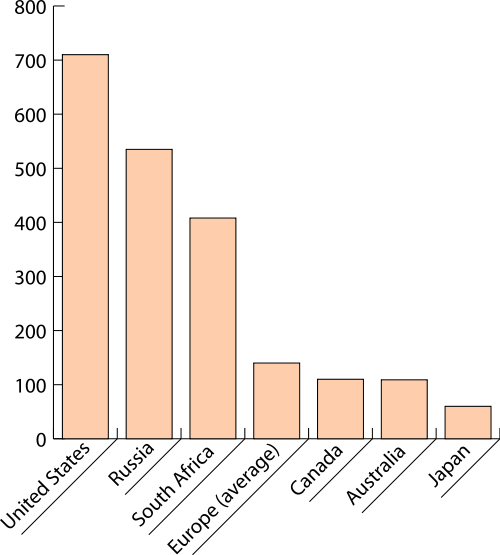
\includegraphics[width=\chartwidth,height=\chartheight]{incarceration}  
\source{Wikipedia}
\end{chart}

\begin{chart}{S}{lr}
\caption{Incarceration ratest across countries}
\label{chart:incarceration}
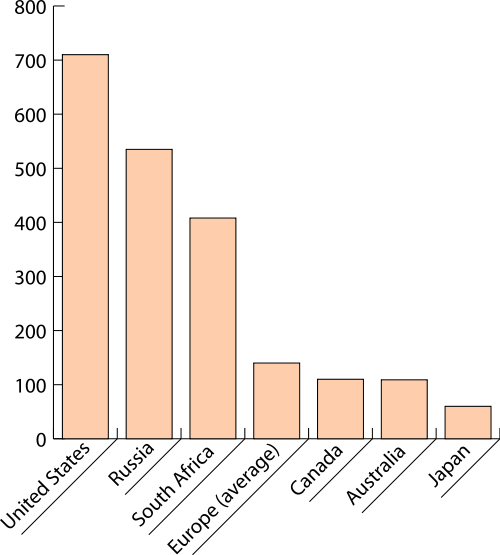
\includegraphics[width=\chartwidth,height=\chartheight]{incarceration}  
\source{Wikipedia}
\end{chart}

\begin{map}{W}{UL}
\caption{Ancient Roma  (Trajan times)}
\label{map:roma}
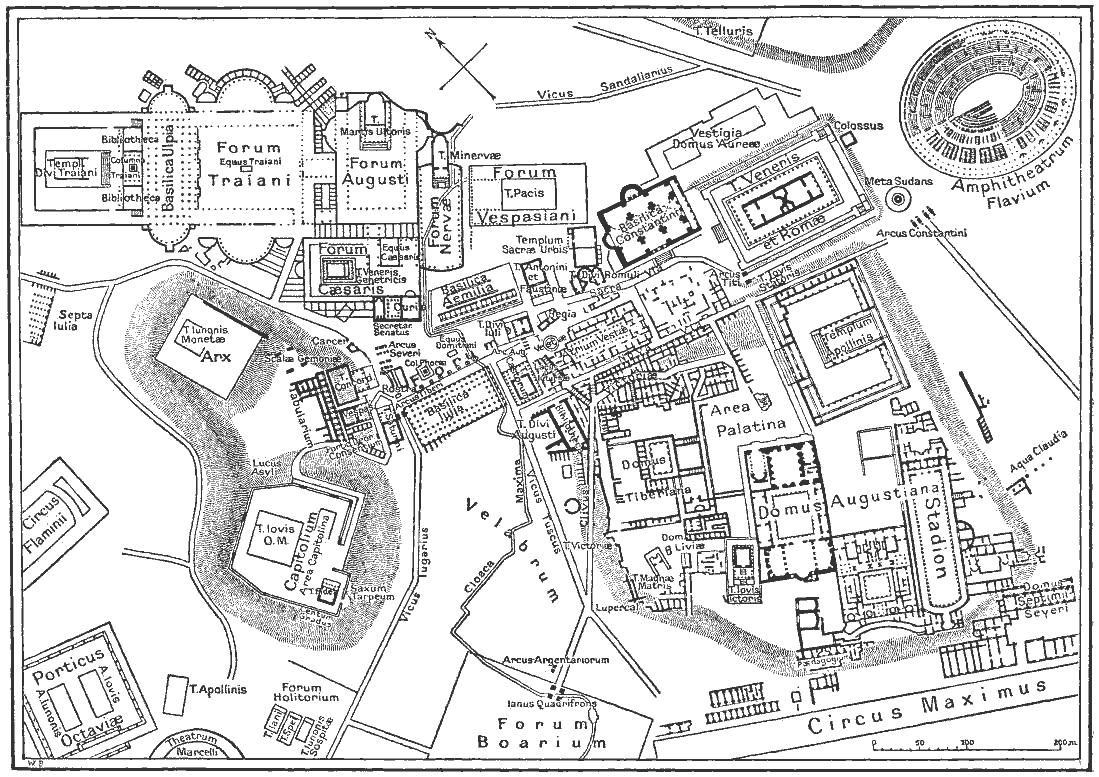
\includegraphics[width=\chartwidth,height=\chartheight]{Rome}
\source{Wikipedia}
\refMetadata{agripop}
\end{map}

\begin{chart}{S}{LL}
\caption{Incarceration ratest across countries}
\label{chart:incarceration}
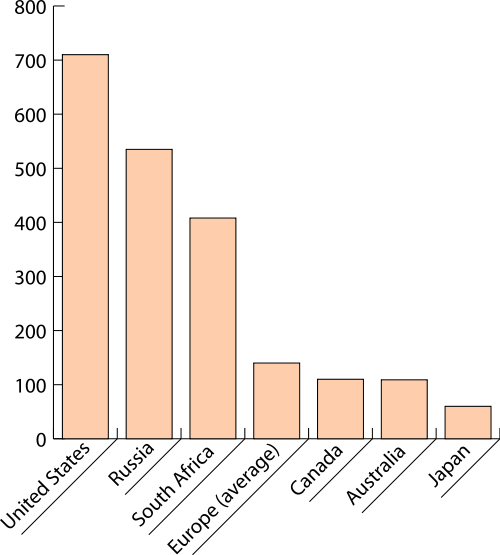
\includegraphics[width=\chartwidth,height=\chartheight]{incarceration}  
\source{Wikipedia}
\end{chart}

\begin{chart}{S}{LR}
\caption{Incarceration ratest across countries}
\label{chart:incarceration}
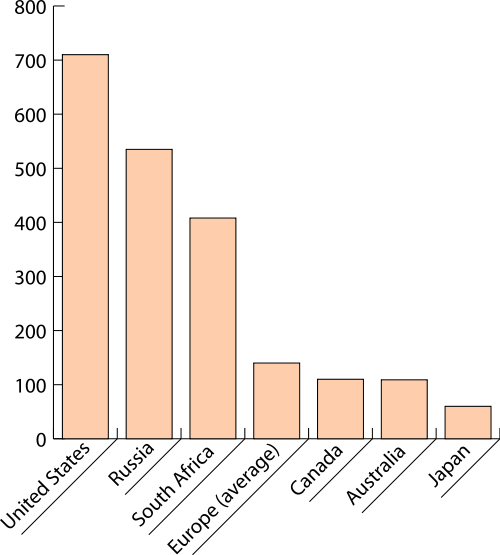
\includegraphics[width=\chartwidth,height=\chartheight]{incarceration}  
\source{Wikipedia}
\end{chart}

%\section{Environment 1B}
%
%\lipsum[1-4]
%%\lipsum[1-5] this breaks it, fills first column
%
%\begin{chart}{S}{ll}
%\caption{Incarceration ratest across countries}
%\label{chart:incarceration}
%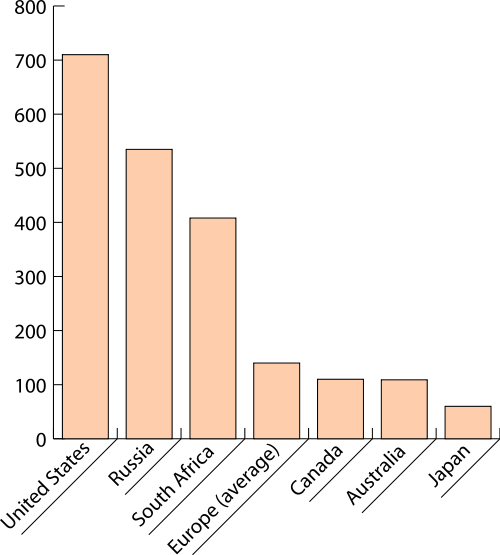
\includegraphics[width=\chartwidth,height=\chartheight]{incarceration}  
%\source{Wikipedia}
%\end{chart}
%
%\begin{chart}{S}{lr}
%\caption{Incarceration ratest across countries}
%\label{chart:incarceration}
%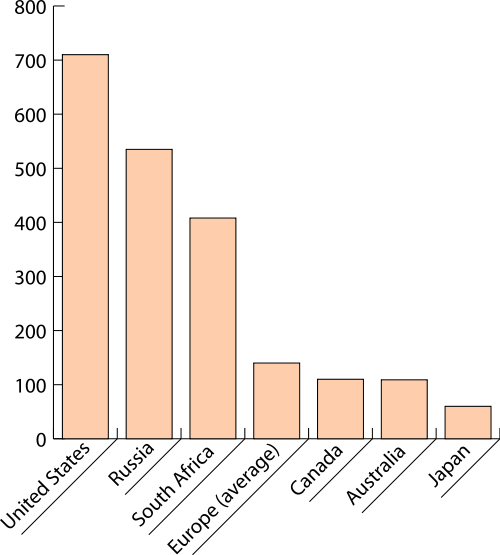
\includegraphics[width=\chartwidth,height=\chartheight]{incarceration}  
%\source{Wikipedia}
%\end{chart}
%
%\begin{chart}{S}{UL}
%\caption{Incarceration ratest across countries}
%\label{chart:incarceration}
%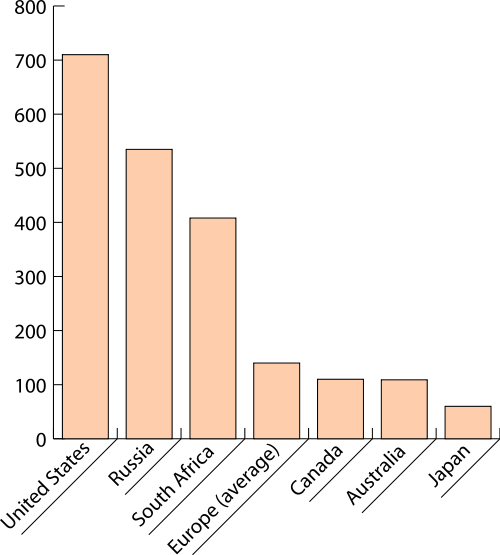
\includegraphics[width=\chartwidth,height=\chartheight]{incarceration}  
%\source{Wikipedia}
%\end{chart}
%
%\begin{chart}{S}{UR}
%\caption{Incarceration ratest across countries}
%\label{chart:incarceration}
%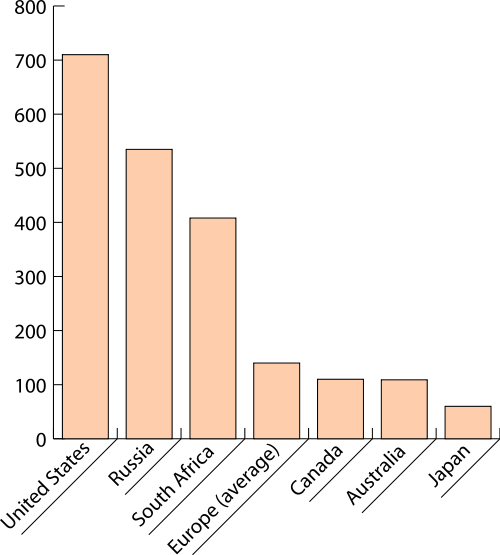
\includegraphics[width=\chartwidth,height=\chartheight]{incarceration}  
%\source{Wikipedia}
%\end{chart}
%
%\begin{map}{W}{LL}
%\caption{Ancient Roma  (Trajan times)}
%\label{map:roma}
%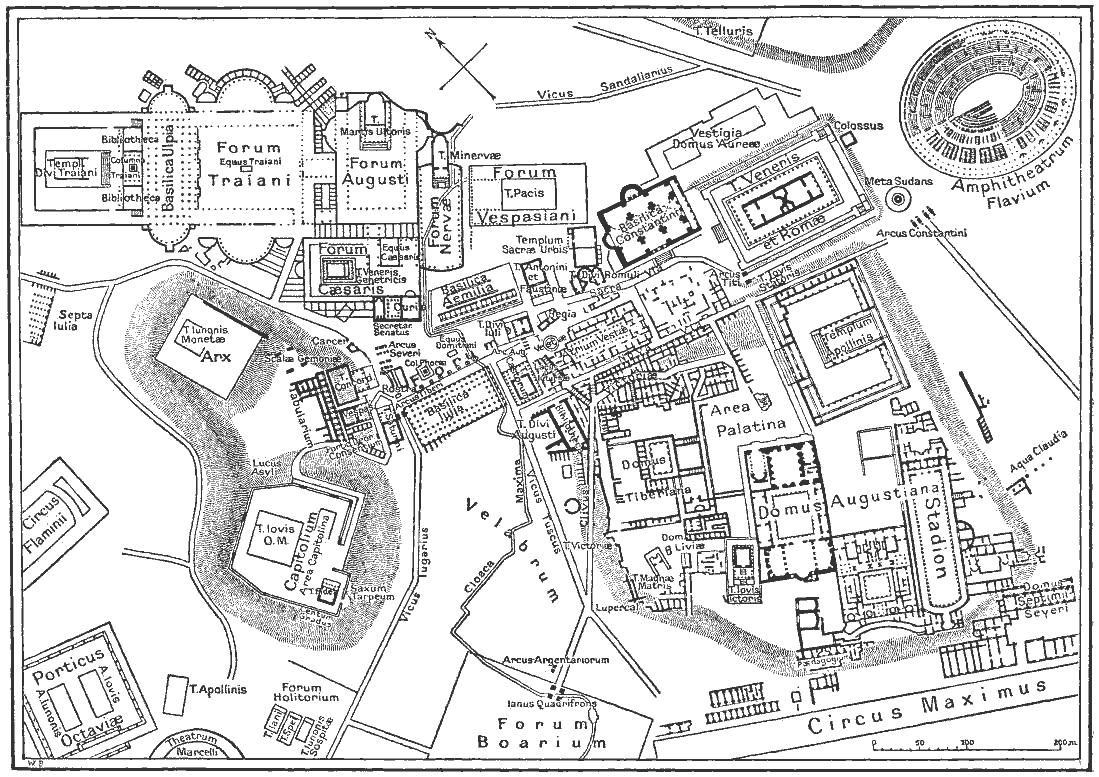
\includegraphics[width=\chartwidth,height=\chartheight]{Rome}
%\source{Wikipedia}
%\refMetadata{agripop}
%\end{map}


%%%%%%%%%%%%%%%%%%%%

\section{Environment 1C}

\lipsum[1-4]
%\lipsum[1-5] this breaks it, fills first column

\begin{chart}{S}{ll}
\caption{Incarceration ratest across countries}
\label{chart:incarceration}
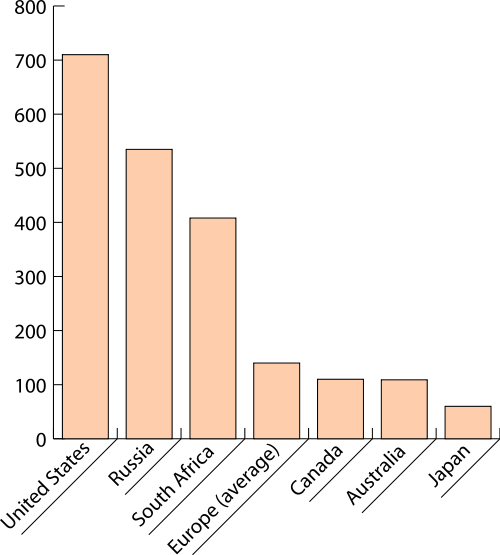
\includegraphics[width=\chartwidth,height=\chartheight]{incarceration}  
\source{Wikipedia}
\end{chart}

\begin{chart}{S}{lr}
\caption{Incarceration ratest across countries}
\label{chart:incarceration}
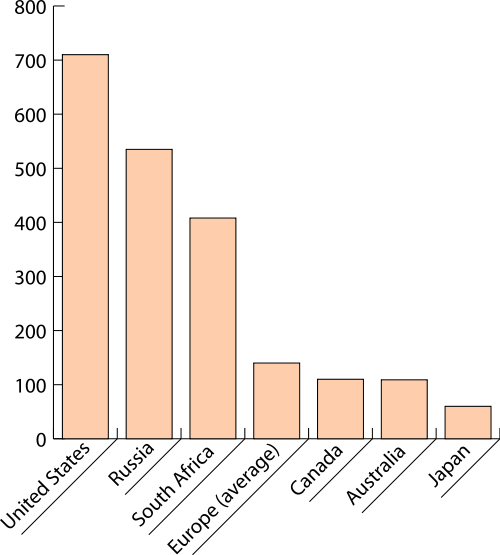
\includegraphics[width=\chartwidth,height=\chartheight]{incarceration}  
\source{Wikipedia}
\end{chart}

\begin{chart}{S}{UL}
\caption{Incarceration ratest across countries}
\label{chart:incarceration}
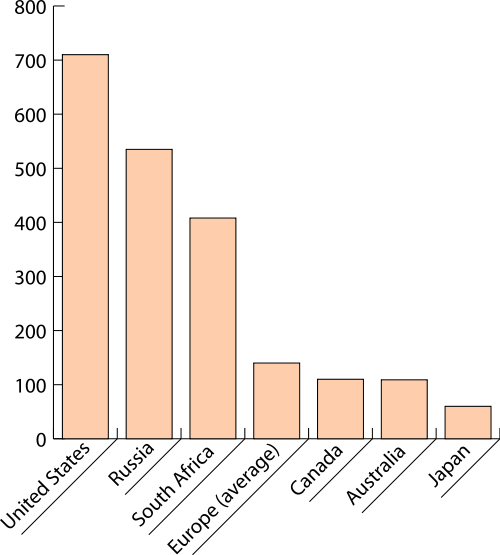
\includegraphics[width=\chartwidth,height=\chartheight]{incarceration}  
\source{Wikipedia}
\end{chart}

\begin{chart}{S}{UR}
\caption{Incarceration ratest across countries}
\label{chart:incarceration}
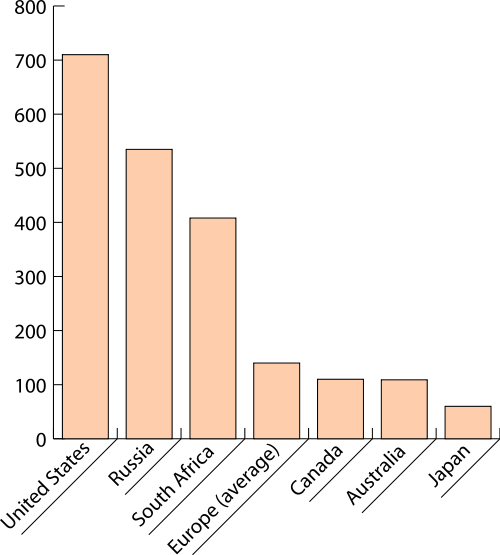
\includegraphics[width=\chartwidth,height=\chartheight]{incarceration}  
\source{Wikipedia}
\end{chart}

\begin{chart}{S}{LR}
\caption{Incarceration ratest across countries}
\label{chart:incarceration}
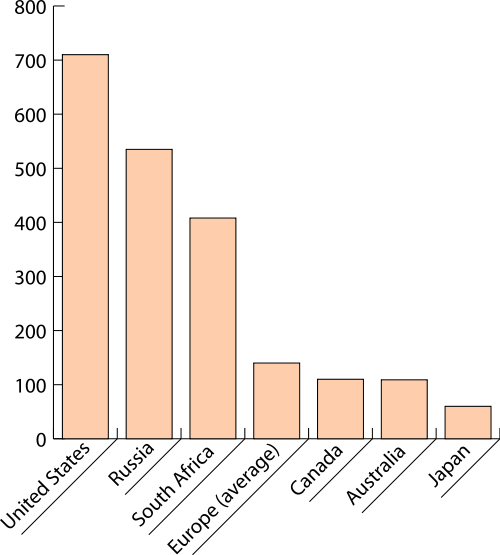
\includegraphics[width=\chartwidth,height=\chartheight]{incarceration}  
\source{Wikipedia}
\end{chart}

\begin{chart}{S}{LL}
\caption{Incarceration ratest across countries}
\label{chart:incarceration}
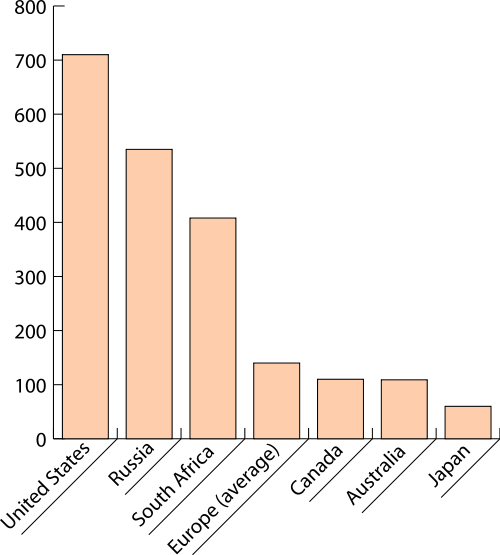
\includegraphics[width=\chartwidth,height=\chartheight]{incarceration}  
\source{Wikipedia}
\end{chart}

%%%%%%%%%%%%%%%%%%%%%%%%%

\section{Environment 1D}

\lipsum[1-4]
%\lipsum[1-5] this breaks it, fills first column

\begin{chart}{S}{ll}
\caption{Incarceration ratest across countries}
\label{chart:incarceration}
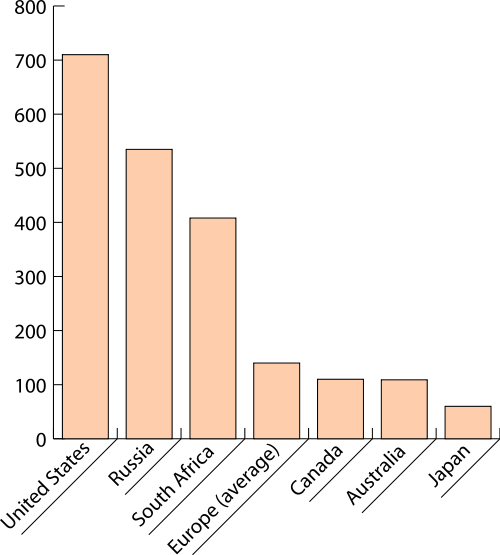
\includegraphics[width=\chartwidth,height=\chartheight]{incarceration}  
\source{Wikipedia}
\end{chart}

\begin{chart}{S}{lr}
\caption{Incarceration ratest across countries}
\label{chart:incarceration}
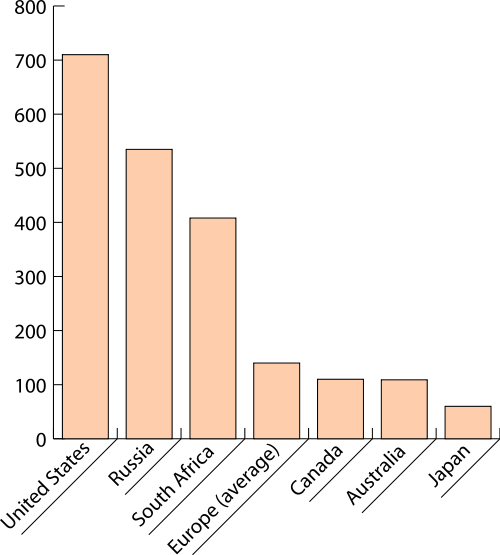
\includegraphics[width=\chartwidth,height=\chartheight]{incarceration}  
\source{Wikipedia}
\end{chart}

\begin{chart}{W}{UL}
\caption{Incarceration ratest across countries}
\label{chart:incarceration}
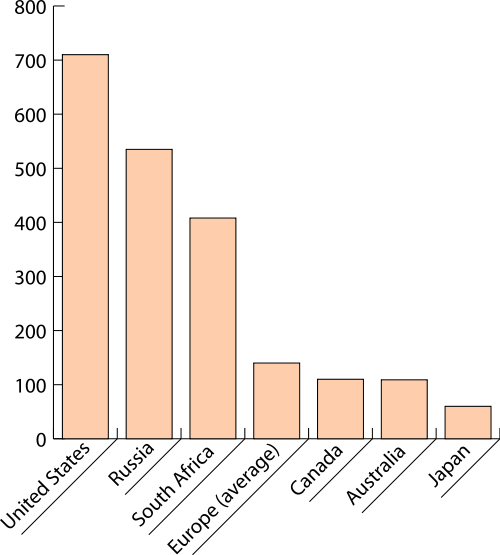
\includegraphics[width=\chartwidth,height=\chartheight]{incarceration}  
\source{Wikipedia}
\end{chart}

\begin{map}{W}{LL}
\caption{Incarceration ratest across countries}
\label{chart:incarceration}
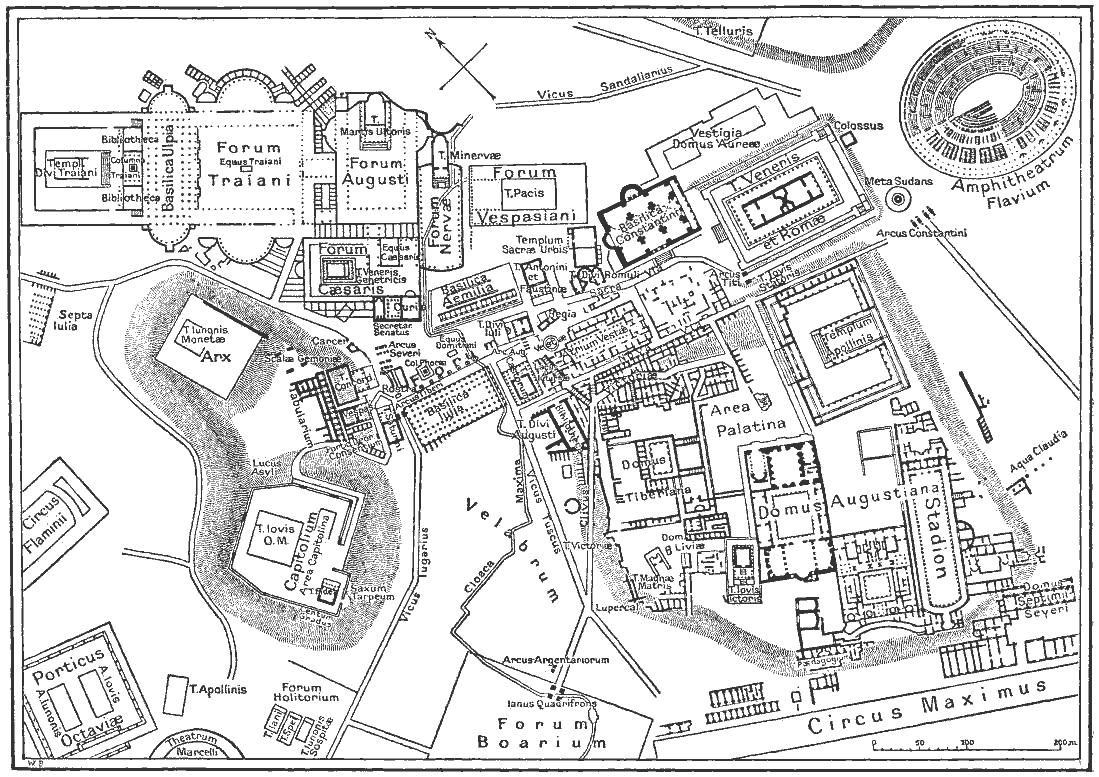
\includegraphics[width=\chartwidth,height=\chartheight]{Rome}  
\source{Wikipedia}
\end{map}

%%%%%%%%%%%%%%%%%%%%%%%%%%%%%%%%

\section{Environment 1E}

\lipsum[1-4]
%\lipsum[1-5] this breaks it, fills first column

\begin{chart}{S}{ll}
\caption{Incarceration ratest across countries}
\label{chart:incarceration}
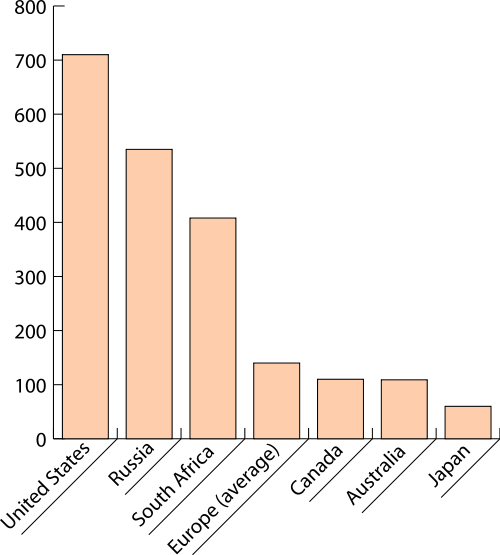
\includegraphics[width=\chartwidth,height=\chartheight]{incarceration}  
\source{Wikipedia}
\end{chart}

\begin{chart}{S}{lr}
\caption{Incarceration ratest across countries}
\label{chart:incarceration}
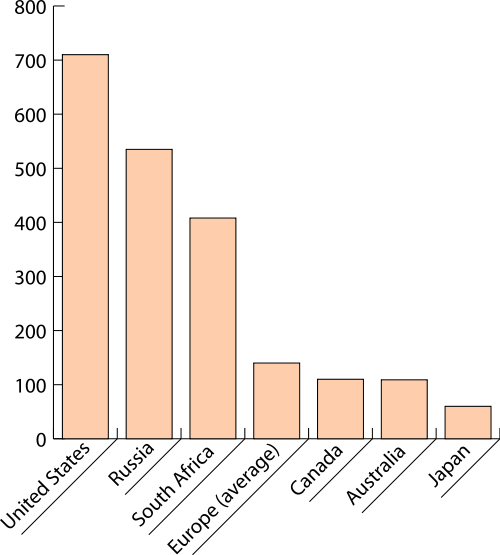
\includegraphics[width=\chartwidth,height=\chartheight]{incarceration}  
\source{Wikipedia}
\end{chart}

\begin{map}{B}{UL}
\caption{Incarceration ratest across countries}
\label{chart:incarceration}
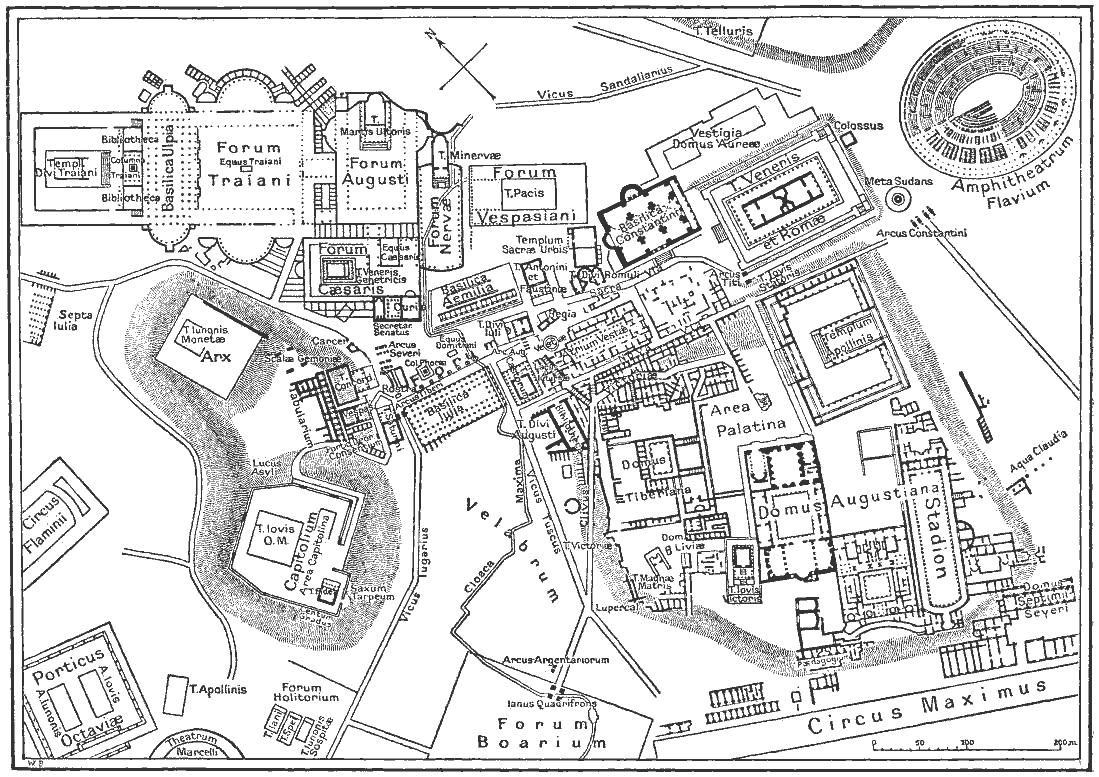
\includegraphics[width=\chartwidth,height=\chartheight]{Rome}  
\source{Wikipedia}
\end{map}

%%%%%%%%%%%%%%%%%%%%%%%%%%%%%%%%%

\section{Environment 2A}

\lipsum[1-2]
%\lipsum[1-5] this breaks it, fills first column

\begin{chart}{S}{ur}
\caption{Incarceration ratest across countries}
\label{chart:incarceration}
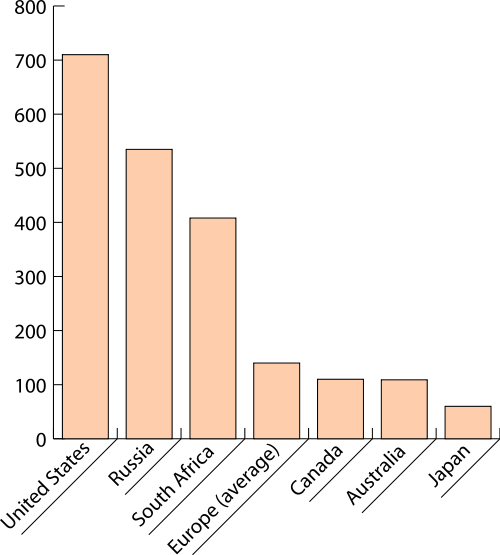
\includegraphics[width=\chartwidth,height=\chartheight]{incarceration}  
\source{Wikipedia}
\end{chart}

\begin{chart}{S}{ll}
\caption{Incarceration ratest across countries}
\label{chart:incarceration}
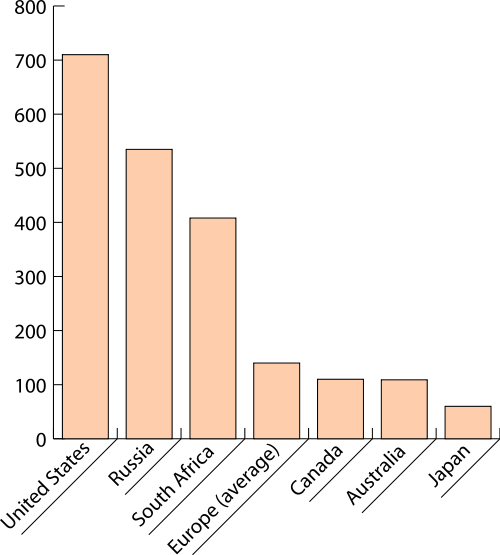
\includegraphics[width=\chartwidth,height=\chartheight]{incarceration}  
\source{Wikipedia}
\end{chart}

\begin{chart}{S}{lr}
\caption{Incarceration ratest across countries}
\label{chart:incarceration}
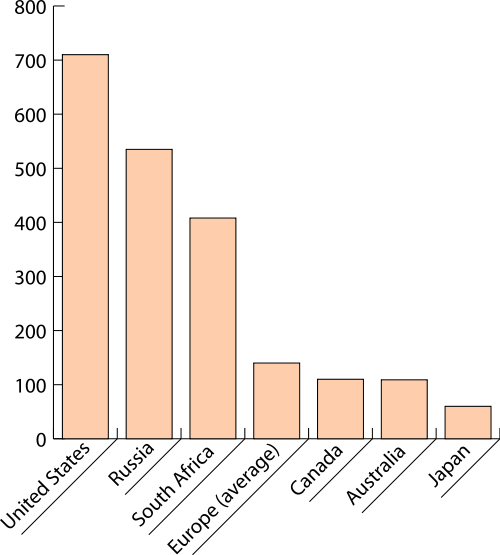
\includegraphics[width=\chartwidth,height=\chartheight]{incarceration}  
\source{Wikipedia}
\end{chart}

\begin{map}{W}{UL}
\caption{Ancient Roma  (Trajan times)}
\label{map:roma}
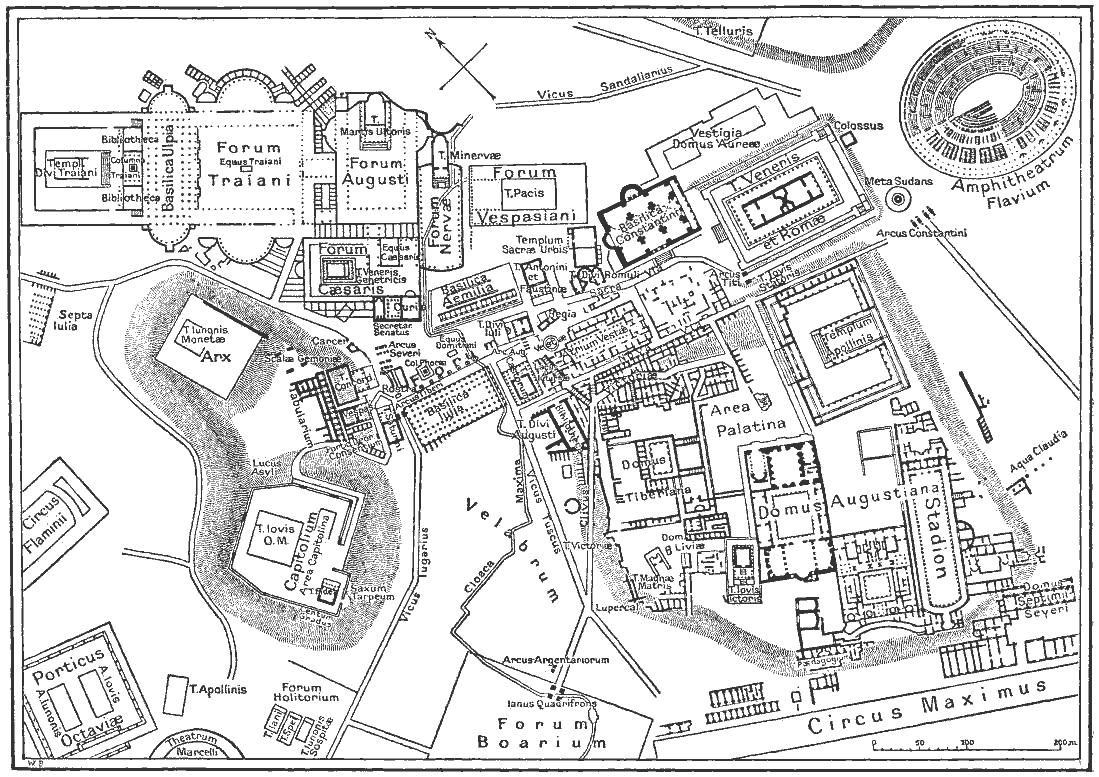
\includegraphics[width=\chartwidth,height=\chartheight]{Rome}
\source{Wikipedia}
\refMetadata{agripop}
\end{map}

\begin{chart}{S}{LL}
\caption{Incarceration ratest across countries}
\label{chart:incarceration}
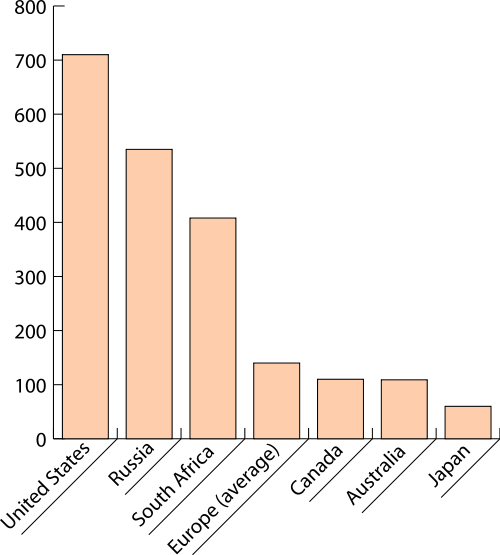
\includegraphics[width=\chartwidth,height=\chartheight]{incarceration}  
\source{Wikipedia}
\end{chart}

\begin{chart}{S}{LR}
\caption{Incarceration ratest across countries}
\label{chart:incarceration}
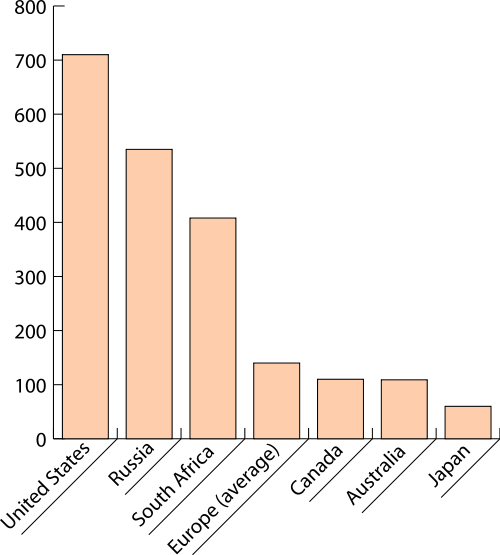
\includegraphics[width=\chartwidth,height=\chartheight]{incarceration}  
\source{Wikipedia}
\end{chart}

%%%%%%%%%%%%%%%%%%%%%%%%%%%%%%%%

%\section{Environment 2B}
%
%\lipsum[1-2]
%
%\begin{chart}{S}{ur}
%\caption{Incarceration ratest across countries}
%\label{chart:incarceration}
%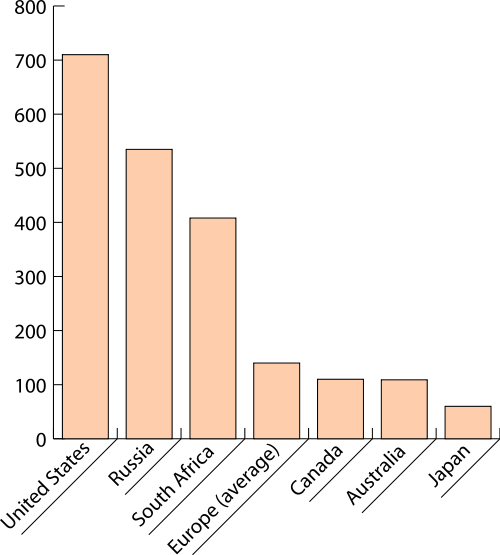
\includegraphics[width=\chartwidth,height=\chartheight]{incarceration}  
%\source{Wikipedia}
%\end{chart}
%
%\begin{chart}{S}{ll}
%\caption{Incarceration ratest across countries}
%\label{chart:incarceration}
%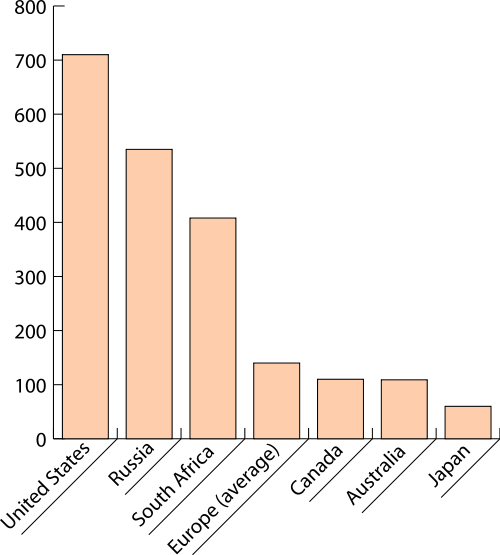
\includegraphics[width=\chartwidth,height=\chartheight]{incarceration}  
%\source{Wikipedia}
%\end{chart}
%
%\begin{chart}{S}{lr}
%\caption{Incarceration ratest across countries}
%\label{chart:incarceration}
%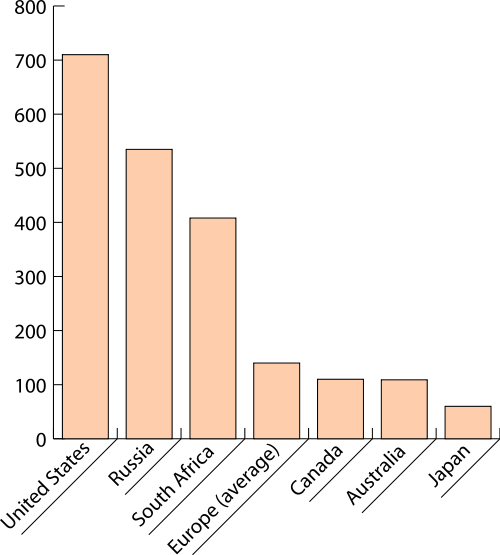
\includegraphics[width=\chartwidth,height=\chartheight]{incarceration}  
%\source{Wikipedia}
%\end{chart}
%
%\begin{chart}{S}{UL}
%\caption{Incarceration ratest across countries}
%\label{chart:incarceration}
%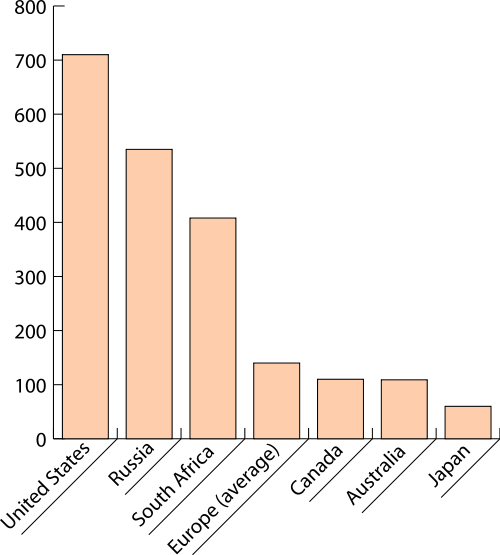
\includegraphics[width=\chartwidth,height=\chartheight]{incarceration}  
%\source{Wikipedia}
%\end{chart}
%
%\begin{chart}{S}{UR}
%\caption{Incarceration ratest across countries}
%\label{chart:incarceration}
%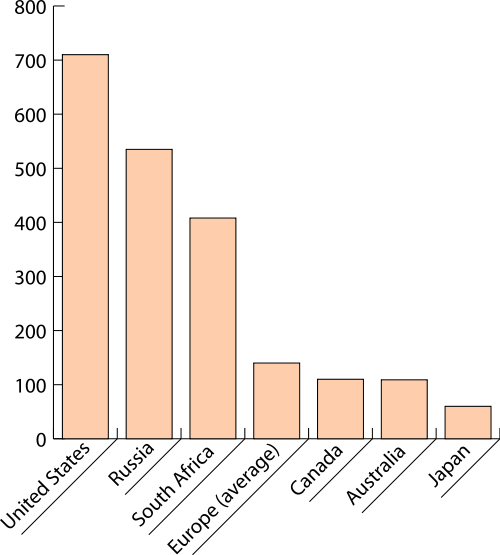
\includegraphics[width=\chartwidth,height=\chartheight]{incarceration}  
%\source{Wikipedia}
%\end{chart}
%
%\begin{map}{W}{LL}
%\caption{Ancient Roma  (Trajan times)}
%\label{map:roma}
%\includegraphics[width=\chartwidth,height=\chartheight]{Rome}
%\source{Wikipedia}
%\refMetadata{agripop}
%\end{map}


%%%%%%%%%%%%%%%%%%%%

\section{Environment 2C}

\lipsum[1-2]
%\lipsum[1-5] this breaks it, fills first column

\begin{chart}{S}{ur}
\caption{Incarceration ratest across countries}
\label{chart:incarceration}
\includegraphics[width=\chartwidth,height=\chartheight]{incarceration}  
\source{Wikipedia}
\end{chart}

\begin{chart}{S}{ll}
\caption{Incarceration ratest across countries}
\label{chart:incarceration}
\includegraphics[width=\chartwidth,height=\chartheight]{incarceration}  
\source{Wikipedia}
\end{chart}

\begin{chart}{S}{lr}
\caption{Incarceration ratest across countries}
\label{chart:incarceration}
\includegraphics[width=\chartwidth,height=\chartheight]{incarceration}  
\source{Wikipedia}
\end{chart}

\begin{chart}{S}{UL}
\caption{Incarceration ratest across countries}
\label{chart:incarceration}
\includegraphics[width=\chartwidth,height=\chartheight]{incarceration}  
\source{Wikipedia}
\end{chart}

\begin{chart}{S}{UR}
\caption{Incarceration ratest across countries}
\label{chart:incarceration}
\includegraphics[width=\chartwidth,height=\chartheight]{incarceration}  
\source{Wikipedia}
\end{chart}

\begin{chart}{S}{LR}
\caption{Incarceration ratest across countries}
\label{chart:incarceration}
\includegraphics[width=\chartwidth,height=\chartheight]{incarceration}  
\source{Wikipedia}
\end{chart}

\begin{chart}{S}{LL}
\caption{Incarceration ratest across countries}
\label{chart:incarceration}
\includegraphics[width=\chartwidth,height=\chartheight]{incarceration}  
\source{Wikipedia}
\end{chart}

%%%%%%%%%%%%%%%%%%%%%%%%%

\section{Environment 2D}

\lipsum[1-2]
%\lipsum[1-5] this breaks it, fills first column

\begin{chart}{S}{ur}
\caption{Incarceration ratest across countries}
\label{chart:incarceration}
\includegraphics[width=\chartwidth,height=\chartheight]{incarceration}  
\source{Wikipedia}
\end{chart}

\begin{chart}{S}{ll}
\caption{Incarceration ratest across countries}
\label{chart:incarceration}
\includegraphics[width=\chartwidth,height=\chartheight]{incarceration}  
\source{Wikipedia}
\end{chart}

\begin{chart}{S}{lr}
\caption{Incarceration ratest across countries}
\label{chart:incarceration}
\includegraphics[width=\chartwidth,height=\chartheight]{incarceration}  
\source{Wikipedia}
\end{chart}

\begin{chart}{W}{UL}
\caption{Incarceration ratest across countries}
\label{chart:incarceration}
\includegraphics[width=\chartwidth,height=\chartheight]{incarceration}  
\source{Wikipedia}
\end{chart}

\begin{map}{W}{LL}
\caption{Incarceration ratest across countries}
\label{chart:incarceration}
\includegraphics[width=\chartwidth,height=\chartheight]{Rome}  
\source{Wikipedia}
\end{map}

%%%%%%%%%%%%%%%%%%%%%%%%%%%%%%%%

\section{Environment 2E}

\lipsum[1-2]
%\lipsum[1-5] this breaks it, fills first column

\begin{chart}{S}{ur}
\caption{Incarceration ratest across countries}
\label{chart:incarceration}
\includegraphics[width=\chartwidth,height=\chartheight]{incarceration}  
\source{Wikipedia}
\end{chart}

\begin{chart}{S}{ll}
\caption{Incarceration ratest across countries}
\label{chart:incarceration}
\includegraphics[width=\chartwidth,height=\chartheight]{incarceration}  
\source{Wikipedia}
\end{chart}

\begin{chart}{S}{lr}
\caption{Incarceration ratest across countries}
\label{chart:incarceration}
\includegraphics[width=\chartwidth,height=\chartheight]{incarceration}  
\source{Wikipedia}
\end{chart}

\begin{map}{B}{UL}
\caption{Incarceration ratest across countries}
\label{chart:incarceration}
\includegraphics[width=\chartwidth,height=\chartheight]{Rome}  
\source{Wikipedia}
\end{map}

%%%%%%%%%%%%%%%%%%%%%%%%%%%%%%%%%

%\section{Environment 3A}
%
%\lipsum[1-4]
%%\lipsum[1-5] this breaks it, fills first column
%
%\begin{map}{W}{ll}
%\caption{Incarceration ratest across countries}
%\label{chart:incarceration}
%\includegraphics[width=\chartwidth,height=\chartheight]{incarceration}  
%\source{Wikipedia}
%\end{map}
%
%\begin{map}{W}{UL}
%\caption{Ancient Roma  (Trajan times)}
%\label{map:roma}
%\includegraphics[width=\chartwidth,height=\chartheight]{Rome}
%\source{Wikipedia}
%\refMetadata{agripop}
%\end{map}

%\begin{chart}{S}{LL}
%\caption{Incarceration ratest across countries}
%\label{chart:incarceration}
%\includegraphics[width=\chartwidth,height=\chartheight]{incarceration}  
%\source{Wikipedia}
%\end{chart}
%
%\begin{chart}{S}{LR}
%\caption{Incarceration ratest across countries}
%\label{chart:incarceration}
%\includegraphics[width=\chartwidth,height=\chartheight]{incarceration}  
%\source{Wikipedia}
%\end{chart}

%
%
%%\section{Environment 3B}
%
%%\lipsum[1-4]
%%%\lipsum[1-5] this breaks it, fills first column
%%
%%\begin{chart}{W}{ll}
%%\caption{Incarceration ratest across countries}
%%\label{chart:incarceration}
%%\includegraphics[width=\chartwidth,height=\chartheight]{incarceration}  
%%\source{Wikipedia}
%%\end{chart}
%%
%%%\begin{chart}{S}{lr}
%%%\caption{Incarceration ratest across countries}
%%%\label{chart:incarceration}
%%%\includegraphics[width=\chartwidth,height=\chartheight]{incarceration}  
%%%\source{Wikipedia}
%%%\end{chart}
%%
%%\begin{chart}{S}{UL}
%%\caption{Incarceration ratest across countries}
%%\label{chart:incarceration}
%%\includegraphics[width=\chartwidth,height=\chartheight]{incarceration}  
%%\source{Wikipedia}
%%\end{chart}
%%
%%\begin{chart}{S}{UR}
%%\caption{Incarceration ratest across countries}
%%\label{chart:incarceration}
%%\includegraphics[width=\chartwidth,height=\chartheight]{incarceration}  
%%\source{Wikipedia}
%%\end{chart}
%%
%%\begin{map}{W}{LL}
%%\caption{Ancient Roma  (Trajan times)}
%%\label{map:roma}
%%\includegraphics[width=\chartwidth,height=\chartheight]{Rome}
%%\source{Wikipedia}
%%\refMetadata{agripop}
%%\end{map}
%
%
%%%%%%%%%%%%%%%%%%%%%
%
%%\section{Environment 3C}
%%
%%\lipsum[1-4]
%%%\lipsum[1-5] this breaks it, fills first column
%%
%%\begin{chart}{W}{ll}
%%\caption{Incarceration ratest across countries}
%%\label{chart:incarceration}
%%\includegraphics[width=\chartwidth,height=\chartheight]{incarceration}  
%%\source{Wikipedia}
%%\end{chart}
%%
%%%\begin{chart}{S}{lr}
%%%\caption{Incarceration ratest across countries}
%%%\label{chart:incarceration}
%%%\includegraphics[width=\chartwidth,height=\chartheight]{incarceration}  
%%%\source{Wikipedia}
%%%\end{chart}
%%
%%\begin{chart}{S}{UL}
%%\caption{Incarceration ratest across countries}
%%\label{chart:incarceration}
%%\includegraphics[width=\chartwidth,height=\chartheight]{incarceration}  
%%\source{Wikipedia}
%%\end{chart}
%%
%%\begin{chart}{S}{UR}
%%\caption{Incarceration ratest across countries}
%%\label{chart:incarceration}
%%\includegraphics[width=\chartwidth,height=\chartheight]{incarceration}  
%%\source{Wikipedia}
%%\end{chart}
%%
%%\begin{chart}{S}{LR}
%%\caption{Incarceration ratest across countries}
%%\label{chart:incarceration}
%%\includegraphics[width=\chartwidth,height=\chartheight]{incarceration}  
%%\source{Wikipedia}
%%\end{chart}
%%
%%\begin{chart}{S}{LL}
%%\caption{Incarceration ratest across countries}
%%\label{chart:incarceration}
%%\includegraphics[width=\chartwidth,height=\chartheight]{incarceration}  
%%\source{Wikipedia}
%%\end{chart}
%%
%%%%%%%%%%%%%%%%%%%%%%%%%%%
%%
%%\section{Environment 3D}
%%
%%\lipsum[1-4]
%%%\lipsum[1-5] this breaks it, fills first column
%%
%%\begin{map}{W}{ll}
%%\caption{Incarceration ratest across countries}
%%\label{chart:incarceration}
%%\includegraphics[width=\chartwidth,height=\chartheight]{incarceration}  
%%\source{Wikipedia}
%%\end{map}
%%%
%%%\begin{chart}{S}{lr}
%%%\caption{Incarceration ratest across countries}
%%%\label{chart:incarceration}
%%%\includegraphics[width=\chartwidth,height=\chartheight]{incarceration}  
%%%\source{Wikipedia}
%%%\end{chart}
%%
%%\begin{chart}{W}{UL}
%%\caption{Incarceration ratest across countries}
%%\label{chart:incarceration}
%%\includegraphics[width=\chartwidth,height=\chartheight]{incarceration}  
%%\source{Wikipedia}
%%\end{chart}
%%
%%\begin{map}{W}{LL}
%%\caption{Incarceration ratest across countries}
%%\label{chart:incarceration}
%%\includegraphics[width=\chartwidth,height=\chartheight]{Rome}  
%%\source{Wikipedia}
%%\end{map}
%%
%%%%%%%%%%%%%%%%%%%%%%%%%%%%%%%%%%
%%
%%\section{Environment 3E}
%%
%%\lipsum[1-4]
%%%\lipsum[1-5] this breaks it, fills first column
%%
%%\begin{chart}{W}{ll}
%%\caption{Incarceration ratest across countries}
%%\label{chart:incarceration}
%%\includegraphics[width=\chartwidth,height=\chartheight]{incarceration}  
%%\source{Wikipedia}
%%\end{chart}
%%
%%%\begin{chart}{S}{lr}
%%%\caption{Incarceration ratest across countries}
%%%\label{chart:incarceration}
%%%\includegraphics[width=\chartwidth,height=\chartheight]{incarceration}  
%%%\source{Wikipedia}
%%%\end{chart}
%%
%%\begin{map}{B}{UL}
%%\caption{Incarceration ratest across countries}
%%\label{chart:incarceration}
%%\includegraphics[width=\chartwidth,height=\chartheight]{Rome}  
%%\source{Wikipedia}
%%\end{map}
%
%%%%%%%%%%%%%%%%%%%%%%%%%%%%%%%%%%
%
%
%%%%%%%%%%%%%%%%%%%%%%%%%%%%%%%%%%

%\section{Environment 4A}
%
%\lipsum[1-2]
%%\lipsum[1-5] this breaks it, fills first column
%
%\begin{map}{S}{ur}
%\caption{Incarceration ratest across countries}
%\label{chart:incarceration}
%\includegraphics[width=\chartwidth,height=\chartheight]{incarceration}  
%\source{Wikipedia}
%\end{map}
%
%\begin{map}{W}{ll}
%\caption{Incarceration ratest across countries}
%\label{chart:incarceration}
%\includegraphics[width=\chartwidth,height=\chartheight]{incarceration}  
%\source{Wikipedia}
%\end{map}
%
%\begin{map}{W}{UL}
%\caption{Ancient Roma  (Trajan times)}
%\label{map:roma}
%\includegraphics[width=\chartwidth,height=\chartheight]{Rome}
%\source{Wikipedia}
%\refMetadata{agripop}
%\end{map}
%
%\begin{chart}{S}{LL}
%\caption{Incarceration ratest across countries}
%\label{chart:incarceration}
%\includegraphics[width=\chartwidth,height=\chartheight]{incarceration}  
%\source{Wikipedia}
%\end{chart}
%
%\begin{chart}{S}{LR}
%\caption{Incarceration ratest across countries}
%\label{chart:incarceration}
%\includegraphics[width=\chartwidth,height=\chartheight]{incarceration}  
%\source{Wikipedia}
%\end{chart}

%%%%%%%%%%%%%%%%%%%%%%%%%%%

\section{Environment 5A}

\lipsum[1-2]
%\lipsum[1-5] this breaks it, fills first column

\begin{map}{T}{ur}
\caption{Incarceration ratest across countries}
\label{chart:incarceration}
\includegraphics[width=\chartwidth,height=\chartheight]{incarceration}  
\source{Wikipedia}
\end{map}

\begin{map}{S}{ll}
\caption{Incarceration ratest across countries}
\label{chart:incarceration}
\includegraphics[width=\chartwidth,height=\chartheight]{incarceration}  
\source{Wikipedia}
\end{map}

\begin{map}{W}{UL}
\caption{Ancient Roma  (Trajan times)}
\label{map:roma}
\includegraphics[width=\chartwidth,height=\chartheight]{Rome}
\source{Wikipedia}
\refMetadata{agripop}
\end{map}

\begin{chart}{S}{LL}
\caption{Incarceration ratest across countries}
\label{chart:incarceration}
\includegraphics[width=\chartwidth,height=\chartheight]{incarceration}  
\source{Wikipedia}
\end{chart}

\begin{chart}{S}{LR}
\caption{Incarceration ratest across countries}
\label{chart:incarceration}
\includegraphics[width=\chartwidth,height=\chartheight]{incarceration}  
\source{Wikipedia}
\end{chart}

%%%%%%%%%%%%%%%%%%%%%%%%%%%

%\section{Environment 5B}
%
%\lipsum[1-2]
%%\lipsum[1-5] this breaks it, fills first column
%
%\begin{map}{T}{ur}
%\caption{Incarceration ratest across countries}
%\label{chart:incarceration}
%\includegraphics[width=\chartwidth,height=\chartheight]{incarceration}  
%\source{Wikipedia}
%\end{map}
%
%\begin{map}{S}{ll}
%\caption{Incarceration ratest across countries}
%\label{chart:incarceration}
%\includegraphics[width=\chartwidth,height=\chartheight]{Rome}  
%\source{Wikipedia}
%\end{map}
%
%\begin{chart}{S}{UL}
%\caption{Incarceration ratest across countries}
%\label{chart:incarceration}
%\includegraphics[width=\chartwidth,height=\chartheight]{incarceration}  
%\source{Wikipedia}
%\end{chart}
%
%\begin{chart}{S}{UR}
%\caption{Incarceration ratest across countries}
%\label{chart:incarceration}
%\includegraphics[width=\chartwidth,height=\chartheight]{incarceration}  
%\source{Wikipedia}
%\end{chart}
%
%\begin{map}{W}{LL}
%\caption{Ancient Roma  (Trajan times)}
%\label{map:roma}
%\includegraphics[width=\chartwidth,height=\chartheight]{Rome}
%\source{Wikipedia}
%\refMetadata{agripop}
%\end{map}

%%%%%%%%%%%%%%%%%%%%%%%%%%%%%%%%%%%

\section{Environment 5C}

\lipsum[1-2]
%\lipsum[1-5] this breaks it, fills first column

\begin{map}{T}{ur}
\caption{Incarceration ratest across countries}
\label{chart:incarceration}
\includegraphics[width=\chartwidth,height=\chartheight]{incarceration}  
\source{Wikipedia}
\end{map}

\begin{map}{S}{ll}
\caption{Incarceration ratest across countries}
\label{chart:incarceration}
\includegraphics[width=\chartwidth,height=\chartheight]{Rome}  
\source{Wikipedia}
\end{map}

\begin{chart}{S}{UL}
\caption{Incarceration ratest across countries}
\label{chart:incarceration}
\includegraphics[width=\chartwidth,height=\chartheight]{incarceration}  
\source{Wikipedia}
\end{chart}

\begin{chart}{S}{UR}
\caption{Incarceration ratest across countries}
\label{chart:incarceration}
\includegraphics[width=\chartwidth,height=\chartheight]{Rome}  
\source{Wikipedia}
\end{chart}

\begin{chart}{S}{LL}
\caption{Incarceration ratest across countries}
\label{chart:incarceration}
\includegraphics[width=\chartwidth,height=\chartheight]{incarceration}  
\source{Wikipedia}
\end{chart}

\begin{chart}{S}{LR}
\caption{Incarceration ratest across countries}
\label{chart:incarceration}
\includegraphics[width=\chartwidth,height=\chartheight]{incarceration}  
\source{Wikipedia}
\end{chart}

%%%%%%%%%%%%%%%%%%%%%%%%%%%%%%%%%%%%

\section{Environment 5D}

\lipsum[1-2]
%\lipsum[1-5] this breaks it, fills first column

\begin{map}{T}{ur}
\caption{Incarceration ratest across countries}
\label{chart:incarceration}
\includegraphics[width=\chartwidth,height=\chartheight]{incarceration}  
\source{Wikipedia}
\end{map}

\begin{map}{S}{ll}
\caption{Incarceration ratest across countries}
\label{chart:incarceration}
\includegraphics[width=\chartwidth,height=\chartheight]{Rome}  
\source{Wikipedia}
\end{map}

\begin{chart}{W}{UL}
\caption{Incarceration ratest across countries}
\label{chart:incarceration}
\includegraphics[width=\chartwidth,height=\chartheight]{incarceration}  
\source{Wikipedia}
\end{chart}

\begin{map}{W}{LL}
\caption{Incarceration ratest across countries}
\label{chart:incarceration}
\includegraphics[width=\chartwidth,height=\chartheight]{Rome}  
\source{Wikipedia}
\end{map}
%
%%%%%%%%%%%%%%%%%%%%%%%%%%%%%%%%%%%%%
%
\section{Environment 5E}

\lipsum[1-2]
%\lipsum[1-5] this breaks it, fills first column

\begin{map}{T}{ur}
\caption{Incarceration ratest across countries}
\label{chart:incarceration}
\includegraphics[width=\chartwidth,height=\chartheight]{incarceration}  
\source{Wikipedia}
\end{map}

\begin{map}{S}{ll}
\caption{Incarceration ratest across countries}
\label{chart:incarceration}
\includegraphics[width=\chartwidth,height=\chartheight]{Rome}  
\source{Wikipedia}
\end{map}

\begin{chart}{B}{UL}
\caption{Incarceration ratest across countries}
\label{chart:incarceration}
\includegraphics[width=\chartwidth,height=\chartheight]{incarceration}  
\source{Wikipedia}
\end{chart}


%%%%%%%%%%%%%%%%%%%%%%%%%%%%%%%%%%%%

\section{Environment 6A}

\lipsum[1-4]

\begin{map}{T}{ur}
\caption{Incarceration ratest across countries}
\label{chart:incarceration}
\includegraphics[width=\chartwidth,height=\chartheight]{incarceration}  
\source{Wikipedia}
\end{map}

\begin{map}{W}{UL}
\caption{Ancient Roma  (Trajan times)}
\label{map:roma}
\includegraphics[width=\chartwidth,height=\chartheight]{Rome}
\source{Wikipedia}
\refMetadata{agripop}
\end{map}

\begin{chart}{S}{LL}
\caption{Incarceration ratest across countries}
\label{chart:incarceration}
\includegraphics[width=\chartwidth,height=\chartheight]{incarceration}  
\source{Wikipedia}
\end{chart}

\begin{chart}{S}{LR}
\caption{Incarceration ratest across countries}
\label{chart:incarceration}
\includegraphics[width=\chartwidth,height=\chartheight]{incarceration}  
\source{Wikipedia}
\end{chart}

%%%%%%%%%%%%%%%%%%%%%%%%%%%

%\section{Environment 6B}
%
%\lipsum[1-2]
%%\lipsum[1-5] this breaks it, fills first column
%
%\begin{map}{T}{ur}
%\caption{Incarceration ratest across countries}
%\label{chart:incarceration}
%\includegraphics[width=\chartwidth,height=\chartheight]{incarceration}  
%\source{Wikipedia}
%\end{map}
%
%\begin{map}{S}{ll}
%\caption{Incarceration ratest across countries}
%\label{chart:incarceration}
%\includegraphics[width=\chartwidth,height=\chartheight]{Rome}  
%\source{Wikipedia}
%\end{map}
%
%\begin{chart}{S}{UL}
%\caption{Incarceration ratest across countries}
%\label{chart:incarceration}
%\includegraphics[width=\chartwidth,height=\chartheight]{incarceration}  
%\source{Wikipedia}
%\end{chart}
%
%\begin{chart}{S}{UR}
%\caption{Incarceration ratest across countries}
%\label{chart:incarceration}
%\includegraphics[width=\chartwidth,height=\chartheight]{incarceration}  
%\source{Wikipedia}
%\end{chart}
%
%\begin{map}{W}{LL}
%\caption{Ancient Roma  (Trajan times)}
%\label{map:roma}
%\includegraphics[width=\chartwidth,height=\chartheight]{Rome}
%\source{Wikipedia}
%\refMetadata{agripop}
%\end{map}

%%%%%%%%%%%%%%%%%%%%%%%%%%%%%%%%%%%

\section{Environment 6C}

\lipsum[1-4]

\begin{map}{T}{ur}
\caption{Incarceration ratest across countries}
\label{chart:incarceration}
\includegraphics[width=\chartwidth,height=\chartheight]{incarceration}  
\source{Wikipedia}
\end{map}

\begin{chart}{S}{UL}
\caption{Incarceration ratest across countries}
\label{chart:incarceration}
\includegraphics[width=\chartwidth,height=\chartheight]{incarceration}  
\source{Wikipedia}
\end{chart}

\begin{chart}{S}{UR}
\caption{Incarceration ratest across countries}
\label{chart:incarceration}
\includegraphics[width=\chartwidth,height=\chartheight]{Rome}  
\source{Wikipedia}
\end{chart}

\begin{chart}{S}{LL}
\caption{Incarceration ratest across countries}
\label{chart:incarceration}
\includegraphics[width=\chartwidth,height=\chartheight]{incarceration}  
\source{Wikipedia}
\end{chart}

\begin{chart}{S}{LR}
\caption{Incarceration ratest across countries}
\label{chart:incarceration}
\includegraphics[width=\chartwidth,height=\chartheight]{incarceration}  
\source{Wikipedia}
\end{chart}

%%%%%%%%%%%%%%%%%%%%%%%%%%%%%%%%%%%%

\section{Environment 6D}

\lipsum[1-4]

\begin{chart}{T}{ur}
\caption{Incarceration ratest across countries}
\label{chart:incarceration}
\includegraphics[width=\chartwidth,height=\chartheight]{incarceration}  
\source{Wikipedia}
\end{chart}

\begin{chart}{W}{UL}
\caption{Incarceration ratest across countries}
\label{chart:incarceration}
\includegraphics[width=\chartwidth,height=\chartheight]{incarceration}  
\source{Wikipedia}
\end{chart}

\begin{map}{W}{LL}
\caption{Incarceration ratest across countries}
\label{chart:incarceration}
\includegraphics[width=\chartwidth,height=\chartheight]{Rome}  
\source{Wikipedia}
\end{map}
%
%%%%%%%%%%%%%%%%%%%%%%%%%%%%%%%%%%%%%
%
\section{Environment 6E}

\lipsum[1-4]

\begin{chart}{T}{ur}
\caption{Incarceration ratest across countries}
\label{chart:incarceration}
\includegraphics[width=\chartwidth,height=\chartheight]{incarceration}  
\source{Wikipedia}
\end{chart}

\begin{chart}{B}{UL}
\caption{Incarceration ratest across countries}
\label{chart:incarceration}
\includegraphics[width=\chartwidth,height=\chartheight]{incarceration}  
\source{Wikipedia}
\end{chart}

%%%%%%%%%%%%%%%%%%%%%%%%%%%%%%%%%%%%%
%
\section{Environment 7A}

\lipsum[1-4]

\begin{chart}{T}{ur}
\caption{Incarceration ratest across countries}
\label{chart:incarceration}
\includegraphics[width=\chartwidth,height=\chartheight]{incarceration}  
\source{Wikipedia}
\end{chart}

\begin{map}{B}{UL}
\caption{Incarceration ratest across countries}
\label{chart:incarceration}
\includegraphics[width=\chartwidth,height=\chartheight]{Rome}  
\source{Wikipedia}
\end{map}



%%%%%%% tabs %%%%%%%%%%%%%

\begin{tablepages}
\section{Inputs}
\small
% latex table generated in R 3.0.0 by xtable 1.7-1 package
% Tue Nov 19 17:29:13 2013
\begin{longtable}{p{3cm}<{\raggedright}d{7.0}d{2.1}d{1.1}d{2.1}d{2.1}d{2.1}d{2.1}d{1.1}d{2.1}}
\caption{Agricultural capital stock\label{T_P1.CAP.1}} \\ 
  
%first line header names
\rowcolor{@tableheadcolor}\cellcolor{white}
&
\multicolumn{9}{H}{\color{white}Gross capital stock} \\[-0.1ex]

%first line header horizontal lines
\hhline{%
	>{\arrayrulecolor{white}}~%
	>{\arrayrulecolor{@tableheadcolor}}|>{\arrayrulecolor{white}}---------%
	>{\arrayrulecolor{@tableheadcolor}}|%
}
%second line header names
\rowcolor{@tableheadcolor} \cellcolor{white} &
\multicolumn{3}{H}{\color{white}total} &
\multicolumn{6}{H}{\color{white}share} \\[-0.1ex]

%second line header horizontal lines
\hhline{%
	>{\arrayrulecolor{white}}~%
	>{\arrayrulecolor{@tableheadcolor}}|>{\arrayrulecolor{white}}---%
	>{\arrayrulecolor{@tableheadcolor}}|>{\arrayrulecolor{white}}------%
	>{\arrayrulecolor{@tableheadcolor}}|%
}
%third line header names
\rowcolor{@tableheadcolor} \cellcolor{white} &
\multicolumn{1}{C{1}}{\color{white} } &
\multicolumn{2}{H}{\color{white}p.a. growth} &
\multicolumn{1}{C{1}}{\color{white}land development} &
\multicolumn{1}{C{1}}{\color{white}plantation crops} &
\multicolumn{1}{C{1}}{\color{white}livestock fixed assets} &
\multicolumn{1}{C{1}}{\color{white}livestock inventory} &
\multicolumn{1}{C{1}}{\color{white}structures for livestock} &
\multicolumn{1}{C{1}}{\color{white}machinery \& equipment}  \\[-0.1ex]

%units in header 
\rowcolor{@tableheadcolor} \cellcolor{white} &
 \multicolumn{1}{C{1}}{\color{white}million US\$} &
 \multicolumn{1}{H}{\color{white}percent} &
 \multicolumn{1}{H}{\color{white}percent} &
 \multicolumn{1}{H}{\color{white}percent} &
 \multicolumn{1}{H}{\color{white}percent} &
 \multicolumn{1}{H}{\color{white}percent} &
 \multicolumn{1}{H}{\color{white}percent} &
 \multicolumn{1}{H}{\color{white}percent} &
 \multicolumn{1}{H}{\color{white}percent}\\ [-0.1ex]
%years in header
\rowcolor{@tableheadcolor} \cellcolor{white} &
 \multicolumn{1}{H}{\color{white}2007} &
 \multicolumn{1}{P{1.5cm}}{\color{white}1990-2000} &
 \multicolumn{1}{H}{\color{white}2000-07} &
 \multicolumn{1}{H}{\color{white}2007} &
 \multicolumn{1}{H}{\color{white}2007} &
 \multicolumn{1}{H}{\color{white}2007} &
 \multicolumn{1}{H}{\color{white}2007} &
 \multicolumn{1}{H}{\color{white}2007} &
 \multicolumn{1}{H}{\color{white}2007}\\ [-0.1ex]
\midrule
\endfirsthead
  \caption[]{Agricultural capital stock (continued)}\\
%first line header names
\rowcolor{@tableheadcolor}\cellcolor{white}
&
\multicolumn{9}{H}{\color{white}Gross capital stock} \\[-0.1ex]

%first line header horizontal lines
\hhline{%
	>{\arrayrulecolor{white}}~%
	>{\arrayrulecolor{@tableheadcolor}}|>{\arrayrulecolor{white}}---------%
	>{\arrayrulecolor{@tableheadcolor}}|%
}
%second line header names
\rowcolor{@tableheadcolor} \cellcolor{white} &
\multicolumn{3}{H}{\color{white}total} &
\multicolumn{6}{H}{\color{white}share} \\[-0.1ex]

%second line header horizontal lines
\hhline{%
	>{\arrayrulecolor{white}}~%
	>{\arrayrulecolor{@tableheadcolor}}|>{\arrayrulecolor{white}}---%
	>{\arrayrulecolor{@tableheadcolor}}|>{\arrayrulecolor{white}}------%
	>{\arrayrulecolor{@tableheadcolor}}|%
}
%third line header names
\rowcolor{@tableheadcolor} \cellcolor{white} &
\multicolumn{1}{C{1}}{\color{white} } &
\multicolumn{2}{H}{\color{white}p.a. growth} &
\multicolumn{1}{C{1}}{\color{white}land development} &
\multicolumn{1}{C{1}}{\color{white}plantation crops} &
\multicolumn{1}{C{1}}{\color{white}livestock fixed assets} &
\multicolumn{1}{C{1}}{\color{white}livestock inventory} &
\multicolumn{1}{C{1}}{\color{white}structures for livestock} &
\multicolumn{1}{C{1}}{\color{white}machinery \& equipment}  \\[-0.1ex]

%units in header 
\rowcolor{@tableheadcolor} \cellcolor{white} &
 \multicolumn{1}{C{1}}{\color{white}million US\$} &
 \multicolumn{1}{H}{\color{white}percent} &
 \multicolumn{1}{H}{\color{white}percent} &
 \multicolumn{1}{H}{\color{white}percent} &
 \multicolumn{1}{H}{\color{white}percent} &
 \multicolumn{1}{H}{\color{white}percent} &
 \multicolumn{1}{H}{\color{white}percent} &
 \multicolumn{1}{H}{\color{white}percent} &
 \multicolumn{1}{H}{\color{white}percent}\\ [-0.1ex]
%years in header
\rowcolor{@tableheadcolor} \cellcolor{white} &
 \multicolumn{1}{H}{\color{white}2007} &
 \multicolumn{1}{P{1.5cm}}{\color{white}1990-2000} &
 \multicolumn{1}{H}{\color{white}2000-07} &
 \multicolumn{1}{H}{\color{white}2007} &
 \multicolumn{1}{H}{\color{white}2007} &
 \multicolumn{1}{H}{\color{white}2007} &
 \multicolumn{1}{H}{\color{white}2007} &
 \multicolumn{1}{H}{\color{white}2007} &
 \multicolumn{1}{H}{\color{white}2007}\\ [-0.1ex]
\midrule 
\endhead
  \bottomrule
\endfoot
\tablemph{Regional office for the Near East} & 335\,938 & 1.9 & 1.2 & 61.9 & 3.3 & 21.9 & 3.9 & 2.3 & 6.7 \\ 
  \tablemph{Gulf Cooperation Council States and Yemen} & 41\,163 & 2.5 & 1.4 & 78.2 & 3.3 & 13.7 & 2.4 & 1.0 & 1.4 \\ 
     \hspace{2pt}\hangindent=4pt\relax Bahrain & 58 & 3.7 & -0.1 & 62.3 & 7.1 & 24.0 & 4.2 & 1.8 & 0.6 \\ 
     \hspace{2pt}\hangindent=4pt\relax Kuwait & 310 & 6.2 & 3.9 & 26.4 & 1.6 & 58.1 & 10.2 & 1.4 & 2.2 \\ 
     \hspace{2pt}\hangindent=4pt\relax Oman & 1\,329 & 2.9 & 0.5 & 42.3 & 4.2 & 41.2 & 7.3 & 3.7 & 1.3 \\ 
     \hspace{2pt}\hangindent=4pt\relax Qatar & 192 & 6.9 & -1.5 & 63.6 & 2.2 & 26.6 & 4.7 & 2.1 & 0.8 \\ 
     \hspace{2pt}\hangindent=4pt\relax Saudi Arabia & 23\,710 & 0.8 & 0.1 & 87.5 & 1.7 & 7.9 & 1.4 & 0.3 & 1.2 \\ 
     \hspace{2pt}\hangindent=4pt\relax United Arab Emirates & 3\,747 & 12.4 & 1.5 & 75.6 & 10.0 & 11.0 & 1.9 & 1.1 & 0.4 \\ 
     \hspace{2pt}\hangindent=4pt\relax Yemen & 11\,815 & 2.8 & 4.0 & 66.0 & 4.4 & 21.7 & 3.8 & 1.9 & 2.2 \\ 
  \tablemph{North Africa} & 62\,717 & 1.0 & 0.6 & 51.0 & 8.5 & 26.1 & 4.6 & 1.5 & 8.3 \\ 
     \hspace{2pt}\hangindent=4pt\relax Algeria & 14\,545 & 1.0 & 1.2 & 42.0 & 6.9 & 28.8 & 5.1 & 1.4 & 15.8 \\ 
     \hspace{2pt}\hangindent=4pt\relax Libya & 7\,531 & -0.1 & 0.7 & 64.6 & 5.6 & 15.4 & 2.7 & 0.5 & 11.1 \\ 
     \hspace{2pt}\hangindent=4pt\relax Mauritania & 4\,331 & 3.1 & 1.2 & 8.9 & 0.3 & 70.9 & 12.5 & 6.6 & 0.7 \\ 
     \hspace{2pt}\hangindent=4pt\relax Morocco & 26\,006 & 0.7 & 0.0 & 63.2 & 4.9 & 22.9 & 4.0 & 1.2 & 3.7 \\ 
     \hspace{2pt}\hangindent=4pt\relax Tunisia & 10\,304 & 1.8 & 0.8 & 40.5 & 25.5 & 19.2 & 3.4 & 0.9 & 10.5 \\ 
  \tablemph{Other Middle East countries} & 232\,058 & 2.1 & 1.4 & 61.9 & 1.9 & 22.2 & 3.9 & 2.8 & 7.2 \\ 
     \hspace{2pt}\hangindent=4pt\relax Egypt & 36\,793 & 2.3 & 1.5 & 73.6 & 2.3 & 15.1 & 2.7 & 2.3 & 4.0 \\ 
     \hspace{2pt}\hangindent=4pt\relax Iran (Islamic Republic of) & 85\,173 & 1.0 & 1.6 & 63.5 & 1.7 & 17.9 & 3.2 & 1.2 & 12.6 \\ 
     \hspace{2pt}\hangindent=4pt\relax Iraq & 31\,881 & -0.0 & 0.2 & 83.2 & 0.9 & 8.8 & 1.5 & 0.5 & 5.1 \\ 
     \hspace{2pt}\hangindent=4pt\relax Jordan & 1\,530 & 1.8 & 1.1 & 51.1 & 7.4 & 27.1 & 4.8 & 0.9 & 8.8 \\ 
     \hspace{2pt}\hangindent=4pt\relax Lebanon & 2\,845 & 0.6 & 0.1 & 73.2 & 16.8 & 6.5 & 1.1 & 0.4 & 2.0 \\ 
     \hspace{2pt}\hangindent=4pt\relax Sudan &  &  &  &  &  &  &  &  &  \\ 
     \hspace{2pt}\hangindent=4pt\relax Sudan (former) & 48\,106 & 4.5 & 1.4 & 29.4 & 0.4 & 50.9 & 9.0 & 9.0 & 1.3 \\ 
     \hspace{2pt}\hangindent=4pt\relax Syrian Arab Republic & 25\,731 & 4.1 & 2.4 & 73.9 & 4.2 & 11.2 & 2.0 & 0.5 & 8.3 \\ 
  \tablemph{Regional Office for Africa} & 430\,811 & 1.8 & 2.0 & 25.5 & 7.3 & 48.0 & 8.5 & 7.7 & 3.0 \\ 
  \tablemph{Regional Office for Asia and the Pacific} & 1\,719\,508 & 0.9 & 0.7 & 32.5 & 10.2 & 25.9 & 4.6 & 4.1 & 22.6 \\ 
  \tablemph{Regional Office for Europe and Central Asia} & 1\,239\,351 &  & -0.4 & 35.2 & 5.8 & 16.5 & 2.9 & 4.3 & 35.3 \\ 
  \tablemph{Regional Office for Latin America and the Caribbean} & 725\,911 & 0.5 & 0.9 & 24.3 & 6.9 & 47.1 & 8.3 & 5.2 & 8.1 \\ 
  \tablemph{World} & 4\,797\,327 & 0.6 & 0.6 & 31.0 & 7.6 & 26.8 & 4.7 & 5.4 & 24.5 \\ 
  \hline
\end{longtable}
  
\clearpage
% latex table generated in R 3.0.0 by xtable 1.7-1 package
% Tue Nov 19 17:35:30 2013
\begin{longtable}{p{3cm}<{\raggedright}d{2.0}d{3.0}d{3.0}d{2.0}d{2.0}d{2.0}d{2.0}d{2.1}d{2.1}}
\caption{Health and education\label{T_P2.HE.1}} \\ 
%first line header names
\rowcolor{@tableheadcolor}\cellcolor{white}
&
\multicolumn{1}{C{1}}{\color{white}Literacy rate} &
\multicolumn{2}{H}{\color{white}Primary completion rate} &
\multicolumn{4}{H}{\color{white}School enrollment} &
\multicolumn{2}{H}{\color{white}Health expenditure} \\[-0.1ex]

%first line header horizontal lines
\hhline{%
	>{\arrayrulecolor{white}}~%
	>{\arrayrulecolor{@tableheadcolor}}|>{\arrayrulecolor{white}}-%
	>{\arrayrulecolor{@tableheadcolor}}|>{\arrayrulecolor{white}}--%
	>{\arrayrulecolor{@tableheadcolor}}|>{\arrayrulecolor{white}}----%
	>{\arrayrulecolor{@tableheadcolor}}|>{\arrayrulecolor{white}}--%
	>{\arrayrulecolor{@tableheadcolor}}|%
}
%second line header names
\rowcolor{@tableheadcolor} \cellcolor{white} &
\multicolumn{1}{C{1}}{\color{white}adult female, \% of females ages 15 +} &
\multicolumn{2}{H}{\color{white}total} &
\multicolumn{4}{H}{\color{white}primary} &
\multicolumn{2}{H}{\color{white}share of GDP} \\[-0.1ex]

%second line header horizontal lines
\hhline{%
	>{\arrayrulecolor{white}}~%
	>{\arrayrulecolor{@tableheadcolor}}|>{\arrayrulecolor{white}}-%
	>{\arrayrulecolor{@tableheadcolor}}|>{\arrayrulecolor{white}}--%
	>{\arrayrulecolor{@tableheadcolor}}|>{\arrayrulecolor{white}}----%
	>{\arrayrulecolor{@tableheadcolor}}|>{\arrayrulecolor{white}}--%
	>{\arrayrulecolor{@tableheadcolor}}|%
}
%third line header names
\rowcolor{@tableheadcolor} \cellcolor{white} &
\multicolumn{1}{C{1}}{\color{white} } &
\multicolumn{2}{H}{\color{white} } &
\multicolumn{2}{H}{\color{white}female} &
\multicolumn{2}{H}{\color{white}male} &
\multicolumn{2}{H}{\color{white} } \\[-0.1ex]

%units in header 
\rowcolor{@tableheadcolor} \cellcolor{white} &
 \multicolumn{1}{H}{\color{white}percent} &
 \multicolumn{1}{H}{\color{white}percent} &
 \multicolumn{1}{H}{\color{white}percent} &
 \multicolumn{1}{H}{\color{white}percent} &
 \multicolumn{1}{H}{\color{white}percent} &
 \multicolumn{1}{H}{\color{white}percent} &
 \multicolumn{1}{H}{\color{white}percent} &
 \multicolumn{1}{H}{\color{white}percent} &
 \multicolumn{1}{H}{\color{white}percent}\\ [-0.1ex]
%years in header
\rowcolor{@tableheadcolor} \cellcolor{white} &
 \multicolumn{1}{H}{\color{white}2005-10*} &
 \multicolumn{1}{H}{\color{white}1990} &
 \multicolumn{1}{H}{\color{white}2010} &
 \multicolumn{1}{H}{\color{white}1990} &
 \multicolumn{1}{H}{\color{white}2010} &
 \multicolumn{1}{H}{\color{white}1990} &
 \multicolumn{1}{H}{\color{white}2010} &
 \multicolumn{1}{H}{\color{white}1995} &
 \multicolumn{1}{H}{\color{white}2010}\\ [-0.1ex]
\midrule
\endfirsthead
  \caption[]{Health and education (continued)}\\
%first line header names
\rowcolor{@tableheadcolor}\cellcolor{white}
&
\multicolumn{1}{C{1}}{\color{white}Literacy rate} &
\multicolumn{2}{H}{\color{white}Primary completion rate} &
\multicolumn{4}{H}{\color{white}School enrollment} &
\multicolumn{2}{H}{\color{white}Health expenditure} \\[-0.1ex]

%first line header horizontal lines
\hhline{%
	>{\arrayrulecolor{white}}~%
	>{\arrayrulecolor{@tableheadcolor}}|>{\arrayrulecolor{white}}-%
	>{\arrayrulecolor{@tableheadcolor}}|>{\arrayrulecolor{white}}--%
	>{\arrayrulecolor{@tableheadcolor}}|>{\arrayrulecolor{white}}----%
	>{\arrayrulecolor{@tableheadcolor}}|>{\arrayrulecolor{white}}--%
	>{\arrayrulecolor{@tableheadcolor}}|%
}
%second line header names
\rowcolor{@tableheadcolor} \cellcolor{white} &
\multicolumn{1}{C{1}}{\color{white}adult female, \% of females ages 15 +} &
\multicolumn{2}{H}{\color{white}total} &
\multicolumn{4}{H}{\color{white}primary} &
\multicolumn{2}{H}{\color{white}share of GDP} \\[-0.1ex]

%second line header horizontal lines
\hhline{%
	>{\arrayrulecolor{white}}~%
	>{\arrayrulecolor{@tableheadcolor}}|>{\arrayrulecolor{white}}-%
	>{\arrayrulecolor{@tableheadcolor}}|>{\arrayrulecolor{white}}--%
	>{\arrayrulecolor{@tableheadcolor}}|>{\arrayrulecolor{white}}----%
	>{\arrayrulecolor{@tableheadcolor}}|>{\arrayrulecolor{white}}--%
	>{\arrayrulecolor{@tableheadcolor}}|%
}
%third line header names
\rowcolor{@tableheadcolor} \cellcolor{white} &
\multicolumn{1}{C{1}}{\color{white} } &
\multicolumn{2}{H}{\color{white} } &
\multicolumn{2}{H}{\color{white}female} &
\multicolumn{2}{H}{\color{white}male} &
\multicolumn{2}{H}{\color{white} } \\[-0.1ex]

%units in header 
\rowcolor{@tableheadcolor} \cellcolor{white} &
 \multicolumn{1}{H}{\color{white}percent} &
 \multicolumn{1}{H}{\color{white}percent} &
 \multicolumn{1}{H}{\color{white}percent} &
 \multicolumn{1}{H}{\color{white}percent} &
 \multicolumn{1}{H}{\color{white}percent} &
 \multicolumn{1}{H}{\color{white}percent} &
 \multicolumn{1}{H}{\color{white}percent} &
 \multicolumn{1}{H}{\color{white}percent} &
 \multicolumn{1}{H}{\color{white}percent}\\ [-0.1ex]
%years in header
\rowcolor{@tableheadcolor} \cellcolor{white} &
 \multicolumn{1}{H}{\color{white}2005-10*} &
 \multicolumn{1}{H}{\color{white}1990} &
 \multicolumn{1}{H}{\color{white}2010} &
 \multicolumn{1}{H}{\color{white}1990} &
 \multicolumn{1}{H}{\color{white}2010} &
 \multicolumn{1}{H}{\color{white}1990} &
 \multicolumn{1}{H}{\color{white}2010} &
 \multicolumn{1}{H}{\color{white}1995} &
 \multicolumn{1}{H}{\color{white}2010}\\ [-0.1ex]
\midrule 
\endhead
  \bottomrule
\endfoot
\tablemph{Africa} &  &  &  &  &  &  &  & 5.1 & 6.0 \\ 
  \tablemph{North Africa} &  &  & 96 &  &  &  &  & 4.1 & 5.2 \\ 
     \hspace{2pt}\hangindent=4pt\relax Algeria & 64 & 81 & 96 & 81 & 95 & 94 & 97 & 4.2 & 4.3 \\ 
     \hspace{2pt}\hangindent=4pt\relax Egypt & 64 &  & 101 &  &  &  &  & 3.9 & 4.7 \\ 
     \hspace{2pt}\hangindent=4pt\relax Libya & 83 &  &  &  &  &  &  & 3.5 &  \\ 
     \hspace{2pt}\hangindent=4pt\relax Morocco & 44 & 52 & 85 & 46 & 93 & 67 & 95 & 3.9 & 5.9 \\ 
     \hspace{2pt}\hangindent=4pt\relax Sudan &  &  &  &  &  &  &  &  & 7.2 \\ 
     \hspace{2pt}\hangindent=4pt\relax Tunisia & 71 & 80 &  & 87 &  & 97 &  & 5.8 & 5.7 \\ 
  \tablemph{Regional Office for Africa} &  &  & 67 &  &  &  &  & 5.7 & 6.5 \\ 
  \tablemph{Central Africa} &  &  & 60 &  &  &  &  & 3.7 & 4.6 \\ 
     \hspace{2pt}\hangindent=4pt\relax Cameroon & 63 & 54 & 79 & 67 & 85 & 76 & 98 & 3.9 & 5.1 \\ 
     \hspace{2pt}\hangindent=4pt\relax Central African Republic & 43 & 30 & 41 & 46 & 60 & 69 & 81 & 3.9 & 3.8 \\ 
     \hspace{2pt}\hangindent=4pt\relax Chad & 24 & 17 & 35 &  &  &  &  & 5.8 & 4.0 \\ 
     \hspace{2pt}\hangindent=4pt\relax Congo &  & 60 & 71 &  & 89 &  & 92 & 3.2 & 2.3 \\ 
     \hspace{2pt}\hangindent=4pt\relax Democratic Republic of the Congo & 57 &  & 59 &  &  &  &  & 3.6 & 7.5 \\ 
     \hspace{2pt}\hangindent=4pt\relax Equatorial Guinea & 91 &  & 52 &  & 56 &  & 57 & 5.9 & 4.2 \\ 
     \hspace{2pt}\hangindent=4pt\relax Gabon & 85 &  &  &  &  &  &  & 3.0 & 3.5 \\ 
     \hspace{2pt}\hangindent=4pt\relax Sao Tome and Principe & 85 & 79 & 85 &  &  &  &  &  & 7.5 \\ 
  \tablemph{East Africa} &  &  & 68 &  &  &  &  & 3.9 & 5.7 \\ 
     \hspace{2pt}\hangindent=4pt\relax Burundi & 62 & 41 & 56 &  &  &  &  & 5.5 & 9.1 \\ 
     \hspace{2pt}\hangindent=4pt\relax Djibouti &  & 32 &  & 25 &  & 33 &  & 4.0 &  \\ 
     \hspace{2pt}\hangindent=4pt\relax Eritrea & 58 &  & 40 &  & 31 &  & 36 & 4.5 & 2.9 \\ 
     \hspace{2pt}\hangindent=4pt\relax Ethiopia & 29 &  & 62 &  & 79 &  & 84 & 2.8 & 4.8 \\ 
     \hspace{2pt}\hangindent=4pt\relax Kenya & 84 &  &  &  &  &  &  & 4.3 & 4.4 \\ 
     \hspace{2pt}\hangindent=4pt\relax Rwanda & 68 & 45 & 70 &  &  &  &  & 4.5 & 10.4 \\ 
     \hspace{2pt}\hangindent=4pt\relax Somalia &  &  &  &  &  &  &  &  &  \\ 
     \hspace{2pt}\hangindent=4pt\relax South Sudan &  &  &  &  &  &  &  &  & 2.1 \\ 
     \hspace{2pt}\hangindent=4pt\relax Sudan (former) & 62 &  &  &  &  &  &  & 3.4 &  \\ 
     \hspace{2pt}\hangindent=4pt\relax Uganda & 65 &  & 57 &  & 92 &  & 90 & 5.8 & 9.2 \\ 
     \hspace{2pt}\hangindent=4pt\relax United Republic of Tanzania & 67 &  & 90 & 52 &  & 51 &  & 3.6 & 7.2 \\ 
  \tablemph{Southern Africa} &  &  & 68 &  &  &  &  & 6.7 & 7.4 \\ 
     \hspace{2pt}\hangindent=4pt\relax Angola & 58 &  & 47 &  & 78 &  & 93 & 5.1 & 3.4 \\ 
     \hspace{2pt}\hangindent=4pt\relax Botswana & 85 & 89 &  & 89 &  & 82 &  & 4.2 & 5.1 \\ 
     \hspace{2pt}\hangindent=4pt\relax Comoros & 70 &  &  &  &  &  &  & 4.7 & 5.3 \\ 
     \hspace{2pt}\hangindent=4pt\relax Lesotho & 96 & 58 & 70 & 78 & 75 & 63 & 72 & 8.1 & 11.5 \\ 
     \hspace{2pt}\hangindent=4pt\relax Madagascar & 62 & 36 & 72 & 69 &  & 70 &  & 2.8 & 3.6 \\ 
     \hspace{2pt}\hangindent=4pt\relax Malawi & 68 & 28 & 68 &  &  &  &  & 5.0 & 8.4 \\ 
     \hspace{2pt}\hangindent=4pt\relax Mauritius & 86 & 111 &  &  &  &  &  & 3.6 & 6.2 \\ 
     \hspace{2pt}\hangindent=4pt\relax Mozambique & 43 & 27 & 61 &  & 89 &  & 94 & 5.3 & 6.3 \\ 
     \hspace{2pt}\hangindent=4pt\relax Namibia & 88 &  & 81 & 83 & 87 & 76 & 83 & 6.2 & 5.5 \\ 
     \hspace{2pt}\hangindent=4pt\relax Seychelles & 92 &  & 133 &  &  &  &  & 5.2 & 3.3 \\ 
     \hspace{2pt}\hangindent=4pt\relax South Africa & 87 &  &  &  &  &  &  & 7.4 & 8.7 \\ 
     \hspace{2pt}\hangindent=4pt\relax Swaziland & 87 & 63 & 77 & 76 &  & 72 &  & 5.0 & 7.8 \\ 
     \hspace{2pt}\hangindent=4pt\relax Zambia & 62 &  & 103 &  & 92 &  & 90 & 5.6 & 6.0 \\ 
     \hspace{2pt}\hangindent=4pt\relax Zimbabwe & 90 &  &  &  &  &  &  & 0.1 &  \\ 
  \tablemph{West Africa} &  &  & 68 &  &  &  &  & 4.8 & 5.7 \\ 
     \hspace{2pt}\hangindent=4pt\relax Benin & 30 & 19 & 70 & 28 &  & 55 &  & 4.7 & 4.3 \\ 
     \hspace{2pt}\hangindent=4pt\relax Burkina Faso & 22 & 18 & 45 &  & 56 &  & 60 & 4.3 & 7.4 \\ 
     \hspace{2pt}\hangindent=4pt\relax Cabo Verde & 79 & 57 & 99 &  & 92 &  & 94 & 5.3 & 4.8 \\ 
     \hspace{2pt}\hangindent=4pt\relax C\^{o}te d'Ivoire & 47 & 40 &  &  &  &  &  & 5.1 & 6.2 \\ 
     \hspace{2pt}\hangindent=4pt\relax Gambia & 40 &  & 70 &  & 67 &  & 64 & 3.3 & 4.4 \\ 
     \hspace{2pt}\hangindent=4pt\relax Ghana & 61 &  &  &  &  &  &  & 5.3 & 5.2 \\ 
     \hspace{2pt}\hangindent=4pt\relax Guinea & 30 & 21 & 64 & 18 & 70 & 36 & 83 & 5.5 & 6.2 \\ 
     \hspace{2pt}\hangindent=4pt\relax Guinea-Bissau & 41 &  & 68 &  & 72 &  & 75 & 6.4 & 7.0 \\ 
     \hspace{2pt}\hangindent=4pt\relax Liberia & 57 &  &  &  &  &  &  & 0.0 & 16.4 \\ 
     \hspace{2pt}\hangindent=4pt\relax Mali & 20 &  & 55 &  & 57 &  & 66 & 5.2 & 6.5 \\ 
     \hspace{2pt}\hangindent=4pt\relax Mauritania & 51 & 29 &  &  & 76 &  & 72 & 4.8 & 6.1 \\ 
     \hspace{2pt}\hangindent=4pt\relax Niger & 15 & 17 & 41 & 18 & 51 & 29 & 63 & 3.4 & 4.8 \\ 
     \hspace{2pt}\hangindent=4pt\relax Nigeria & 50 &  & 74 &  & 55 &  & 60 & 4.5 & 5.4 \\ 
     \hspace{2pt}\hangindent=4pt\relax Senegal & 39 & 43 & 59 & 39 & 78 & 53 & 73 & 3.9 & 5.8 \\ 
     \hspace{2pt}\hangindent=4pt\relax Sierra Leone & 31 &  &  &  &  &  &  & 15.3 & 20.8 \\ 
     \hspace{2pt}\hangindent=4pt\relax Togo & 44 & 38 & 74 & 55 &  & 79 &  & 4.6 & 7.5 \\ 
  \tablemph{CEMAC} &  & 42 & 61 &  &  &  &  & 3.7 & 4.0 \\ 
  \tablemph{CEN-SAD} &  &  &  &  &  &  &  & 4.2 & 5.5 \\ 
  \tablemph{COMESA} &  &  &  &  &  &  &  & 3.7 & 5.4 \\ 
  \tablemph{ECCAS} &  &  & 57 &  &  &  &  & 4.0 & 4.0 \\ 
  \tablemph{ECOWAS} &  &  & 68 &  &  &  &  & 4.8 & 5.7 \\ 
  \tablemph{IGAD} &  &  &  &  &  &  &  & 3.9 & 5.9 \\ 
  \tablemph{SADC} &  &  & 70 &  &  &  &  & 6.5 & 7.4 \\ 
  \tablemph{UEMOA} &  & 30 & 54 &  &  &  &  & 4.6 & 6.1 \\ 
  \tablemph{UMA} &  & 67 &  &  &  &  &  & 4.2 & 5.0 \\ 
  \tablemph{Regional Office for Asia and the Pacific} &  &  &  &  &  &  &  & 5.8 & 6.4 \\ 
  \tablemph{Regional Office for Europe and Central Asia} &  &  & 99 &  &  &  &  & 8.4 & 9.8 \\ 
  \tablemph{Regional Office for Latin America and the Caribbean} &  &  & 102 &  &  &  &  & 6.5 & 7.6 \\ 
  \tablemph{Regional Office for the Near East} &  &  &  &  &  &  &  & 3.8 & 4.6 \\ 
  \tablemph{World} &  &  &  &  &  &  &  & 8.8 & 10.3 \\ 
  \hline
\end{longtable}

\end{tablepages}

%%%%%%%%%%%%%%%%%%% PART 2: HUNGER DIMENSIONS %%%%%%%%%%%%%%

\faoset{bgcolor=part2,icon=icons/hunger}
\part{Hunger Dimensions}
\lipsum
\EndPartIntro

\section{Environment 1A}

\lipsum[1-4]
%\lipsum[1-5] this breaks it, fills first column

\begin{chart}{S}{ll}
\caption{Incarceration ratest across countries}
\label{chart:incarceration}
\includegraphics[width=\chartwidth,height=\chartheight]{incarceration}  
\source{Wikipedia}
\end{chart}

\begin{chart}{S}{lr}
\caption{Incarceration ratest across countries}
\label{chart:incarceration}
\includegraphics[width=\chartwidth,height=\chartheight]{incarceration}  
\source{Wikipedia}
\end{chart}

\begin{map}{W}{UL}
\caption{Ancient Roma  (Trajan times)}
\label{map:roma}
\includegraphics[width=\chartwidth,height=\chartheight]{Rome}
\source{Wikipedia}
\refMetadata{agripop}
\end{map}

\begin{chart}{S}{LL}
\caption{Incarceration ratest across countries}
\label{chart:incarceration}
\includegraphics[width=\chartwidth,height=\chartheight]{incarceration}  
\source{Wikipedia}
\end{chart}

\begin{chart}{S}{LR}
\caption{Incarceration ratest across countries}
\label{chart:incarceration}
\includegraphics[width=\chartwidth,height=\chartheight]{incarceration}  
\source{Wikipedia}
\end{chart}

%\section{Environment 1B}
%
%\lipsum[1-4]
%%\lipsum[1-5] this breaks it, fills first column
%
%\begin{chart}{S}{ll}
%\caption{Incarceration ratest across countries}
%\label{chart:incarceration}
%\includegraphics[width=\chartwidth,height=\chartheight]{incarceration}  
%\source{Wikipedia}
%\end{chart}
%
%\begin{chart}{S}{lr}
%\caption{Incarceration ratest across countries}
%\label{chart:incarceration}
%\includegraphics[width=\chartwidth,height=\chartheight]{incarceration}  
%\source{Wikipedia}
%\end{chart}
%
%\begin{chart}{S}{UL}
%\caption{Incarceration ratest across countries}
%\label{chart:incarceration}
%\includegraphics[width=\chartwidth,height=\chartheight]{incarceration}  
%\source{Wikipedia}
%\end{chart}
%
%\begin{chart}{S}{UR}
%\caption{Incarceration ratest across countries}
%\label{chart:incarceration}
%\includegraphics[width=\chartwidth,height=\chartheight]{incarceration}  
%\source{Wikipedia}
%\end{chart}
%
%\begin{map}{W}{LL}
%\caption{Ancient Roma  (Trajan times)}
%\label{map:roma}
%\includegraphics[width=\chartwidth,height=\chartheight]{Rome}
%\source{Wikipedia}
%\refMetadata{agripop}
%\end{map}


%%%%%%%%%%%%%%%%%%%%

\section{Environment 1C}

\lipsum[1-4]
%\lipsum[1-5] this breaks it, fills first column

\begin{chart}{S}{ll}
\caption{Incarceration ratest across countries}
\label{chart:incarceration}
\includegraphics[width=\chartwidth,height=\chartheight]{incarceration}  
\source{Wikipedia}
\end{chart}

\begin{chart}{S}{lr}
\caption{Incarceration ratest across countries}
\label{chart:incarceration}
\includegraphics[width=\chartwidth,height=\chartheight]{incarceration}  
\source{Wikipedia}
\end{chart}

\begin{chart}{S}{UL}
\caption{Incarceration ratest across countries}
\label{chart:incarceration}
\includegraphics[width=\chartwidth,height=\chartheight]{incarceration}  
\source{Wikipedia}
\end{chart}

\begin{chart}{S}{UR}
\caption{Incarceration ratest across countries}
\label{chart:incarceration}
\includegraphics[width=\chartwidth,height=\chartheight]{incarceration}  
\source{Wikipedia}
\end{chart}

\begin{chart}{S}{LR}
\caption{Incarceration ratest across countries}
\label{chart:incarceration}
\includegraphics[width=\chartwidth,height=\chartheight]{incarceration}  
\source{Wikipedia}
\end{chart}

\begin{chart}{S}{LL}
\caption{Incarceration ratest across countries}
\label{chart:incarceration}
\includegraphics[width=\chartwidth,height=\chartheight]{incarceration}  
\source{Wikipedia}
\end{chart}

%%%%%%%%%%%%%%%%%%%%%%%%%

\section{Environment 1D}

\lipsum[1-4]
%\lipsum[1-5] this breaks it, fills first column

\begin{chart}{S}{ll}
\caption{Incarceration ratest across countries}
\label{chart:incarceration}
\includegraphics[width=\chartwidth,height=\chartheight]{incarceration}  
\source{Wikipedia}
\end{chart}

\begin{chart}{S}{lr}
\caption{Incarceration ratest across countries}
\label{chart:incarceration}
\includegraphics[width=\chartwidth,height=\chartheight]{incarceration}  
\source{Wikipedia}
\end{chart}

\begin{chart}{W}{UL}
\caption{Incarceration ratest across countries}
\label{chart:incarceration}
\includegraphics[width=\chartwidth,height=\chartheight]{incarceration}  
\source{Wikipedia}
\end{chart}

\begin{map}{W}{LL}
\caption{Incarceration ratest across countries}
\label{chart:incarceration}
\includegraphics[width=\chartwidth,height=\chartheight]{Rome}  
\source{Wikipedia}
\end{map}

%%%%%%%%%%%%%%%%%%%%%%%%%%%%%%%%

\section{Environment 1E}

\lipsum[1-4]
%\lipsum[1-5] this breaks it, fills first column

\begin{chart}{S}{ll}
\caption{Incarceration ratest across countries}
\label{chart:incarceration}
\includegraphics[width=\chartwidth,height=\chartheight]{incarceration}  
\source{Wikipedia}
\end{chart}

\begin{chart}{S}{lr}
\caption{Incarceration ratest across countries}
\label{chart:incarceration}
\includegraphics[width=\chartwidth,height=\chartheight]{incarceration}  
\source{Wikipedia}
\end{chart}

\begin{map}{B}{UL}
\caption{Incarceration ratest across countries}
\label{chart:incarceration}
\includegraphics[width=\chartwidth,height=\chartheight]{Rome}  
\source{Wikipedia}
\end{map}

%%%%%%%%%%%%%%%%%%%%%%%%%%%%%%%%%

\section{Environment 2A}

\lipsum[1-2]
%\lipsum[1-5] this breaks it, fills first column

\begin{chart}{S}{ur}
\caption{Incarceration ratest across countries}
\label{chart:incarceration}
\includegraphics[width=\chartwidth,height=\chartheight]{incarceration}  
\source{Wikipedia}
\end{chart}

\begin{chart}{S}{ll}
\caption{Incarceration ratest across countries}
\label{chart:incarceration}
\includegraphics[width=\chartwidth,height=\chartheight]{incarceration}  
\source{Wikipedia}
\end{chart}

\begin{chart}{S}{lr}
\caption{Incarceration ratest across countries}
\label{chart:incarceration}
\includegraphics[width=\chartwidth,height=\chartheight]{incarceration}  
\source{Wikipedia}
\end{chart}

\begin{map}{W}{UL}
\caption{Ancient Roma  (Trajan times)}
\label{map:roma}
\includegraphics[width=\chartwidth,height=\chartheight]{Rome}
\source{Wikipedia}
\refMetadata{agripop}
\end{map}

\begin{chart}{S}{LL}
\caption{Incarceration ratest across countries}
\label{chart:incarceration}
\includegraphics[width=\chartwidth,height=\chartheight]{incarceration}  
\source{Wikipedia}
\end{chart}

\begin{chart}{S}{LR}
\caption{Incarceration ratest across countries}
\label{chart:incarceration}
\includegraphics[width=\chartwidth,height=\chartheight]{incarceration}  
\source{Wikipedia}
\end{chart}

%%%%%%%%%%%%%%%%%%%%%%%%%%%%%%%%

%\section{Environment 2B}
%
%\lipsum[1-2]
%
%\begin{chart}{S}{ur}
%\caption{Incarceration ratest across countries}
%\label{chart:incarceration}
%\includegraphics[width=\chartwidth,height=\chartheight]{incarceration}  
%\source{Wikipedia}
%\end{chart}
%
%\begin{chart}{S}{ll}
%\caption{Incarceration ratest across countries}
%\label{chart:incarceration}
%\includegraphics[width=\chartwidth,height=\chartheight]{incarceration}  
%\source{Wikipedia}
%\end{chart}
%
%\begin{chart}{S}{lr}
%\caption{Incarceration ratest across countries}
%\label{chart:incarceration}
%\includegraphics[width=\chartwidth,height=\chartheight]{incarceration}  
%\source{Wikipedia}
%\end{chart}
%
%\begin{chart}{S}{UL}
%\caption{Incarceration ratest across countries}
%\label{chart:incarceration}
%\includegraphics[width=\chartwidth,height=\chartheight]{incarceration}  
%\source{Wikipedia}
%\end{chart}
%
%\begin{chart}{S}{UR}
%\caption{Incarceration ratest across countries}
%\label{chart:incarceration}
%\includegraphics[width=\chartwidth,height=\chartheight]{incarceration}  
%\source{Wikipedia}
%\end{chart}
%
%\begin{map}{W}{LL}
%\caption{Ancient Roma  (Trajan times)}
%\label{map:roma}
%\includegraphics[width=\chartwidth,height=\chartheight]{Rome}
%\source{Wikipedia}
%\refMetadata{agripop}
%\end{map}


%%%%%%%%%%%%%%%%%%%%

\section{Environment 2C}

\lipsum[1-2]
%\lipsum[1-5] this breaks it, fills first column

\begin{chart}{S}{ur}
\caption{Incarceration ratest across countries}
\label{chart:incarceration}
\includegraphics[width=\chartwidth,height=\chartheight]{incarceration}  
\source{Wikipedia}
\end{chart}

\begin{chart}{S}{ll}
\caption{Incarceration ratest across countries}
\label{chart:incarceration}
\includegraphics[width=\chartwidth,height=\chartheight]{incarceration}  
\source{Wikipedia}
\end{chart}

\begin{chart}{S}{lr}
\caption{Incarceration ratest across countries}
\label{chart:incarceration}
\includegraphics[width=\chartwidth,height=\chartheight]{incarceration}  
\source{Wikipedia}
\end{chart}

\begin{chart}{S}{UL}
\caption{Incarceration ratest across countries}
\label{chart:incarceration}
\includegraphics[width=\chartwidth,height=\chartheight]{incarceration}  
\source{Wikipedia}
\end{chart}

\begin{chart}{S}{UR}
\caption{Incarceration ratest across countries}
\label{chart:incarceration}
\includegraphics[width=\chartwidth,height=\chartheight]{incarceration}  
\source{Wikipedia}
\end{chart}

\begin{chart}{S}{LR}
\caption{Incarceration ratest across countries}
\label{chart:incarceration}
\includegraphics[width=\chartwidth,height=\chartheight]{incarceration}  
\source{Wikipedia}
\end{chart}

\begin{chart}{S}{LL}
\caption{Incarceration ratest across countries}
\label{chart:incarceration}
\includegraphics[width=\chartwidth,height=\chartheight]{incarceration}  
\source{Wikipedia}
\end{chart}

%%%%%%%%%%%%%%%%%%%%%%%%%

\section{Environment 2D}

\lipsum[1-2]
%\lipsum[1-5] this breaks it, fills first column

\begin{chart}{S}{ur}
\caption{Incarceration ratest across countries}
\label{chart:incarceration}
\includegraphics[width=\chartwidth,height=\chartheight]{incarceration}  
\source{Wikipedia}
\end{chart}

\begin{chart}{S}{ll}
\caption{Incarceration ratest across countries}
\label{chart:incarceration}
\includegraphics[width=\chartwidth,height=\chartheight]{incarceration}  
\source{Wikipedia}
\end{chart}

\begin{chart}{S}{lr}
\caption{Incarceration ratest across countries}
\label{chart:incarceration}
\includegraphics[width=\chartwidth,height=\chartheight]{incarceration}  
\source{Wikipedia}
\end{chart}

\begin{chart}{W}{UL}
\caption{Incarceration ratest across countries}
\label{chart:incarceration}
\includegraphics[width=\chartwidth,height=\chartheight]{incarceration}  
\source{Wikipedia}
\end{chart}

\begin{map}{W}{LL}
\caption{Incarceration ratest across countries}
\label{chart:incarceration}
\includegraphics[width=\chartwidth,height=\chartheight]{Rome}  
\source{Wikipedia}
\end{map}

%%%%%%%%%%%%%%%%%%%%%%%%%%%%%%%%

\section{Environment 2E}

\lipsum[1-2]
%\lipsum[1-5] this breaks it, fills first column

\begin{chart}{S}{ur}
\caption{Incarceration ratest across countries}
\label{chart:incarceration}
\includegraphics[width=\chartwidth,height=\chartheight]{incarceration}  
\source{Wikipedia}
\end{chart}

\begin{chart}{S}{ll}
\caption{Incarceration ratest across countries}
\label{chart:incarceration}
\includegraphics[width=\chartwidth,height=\chartheight]{incarceration}  
\source{Wikipedia}
\end{chart}

\begin{chart}{S}{lr}
\caption{Incarceration ratest across countries}
\label{chart:incarceration}
\includegraphics[width=\chartwidth,height=\chartheight]{incarceration}  
\source{Wikipedia}
\end{chart}

\begin{map}{B}{UL}
\caption{Incarceration ratest across countries}
\label{chart:incarceration}
\includegraphics[width=\chartwidth,height=\chartheight]{Rome}  
\source{Wikipedia}
\end{map}

%%%%%%%%%%%%%%%%%%%%%%%%%%%%%%%%%

%\section{Environment 3A}
%
%\lipsum[1-4]
%%\lipsum[1-5] this breaks it, fills first column
%
%\begin{map}{W}{ll}
%\caption{Incarceration ratest across countries}
%\label{chart:incarceration}
%\includegraphics[width=\chartwidth,height=\chartheight]{incarceration}  
%\source{Wikipedia}
%\end{map}
%
%\begin{map}{W}{UL}
%\caption{Ancient Roma  (Trajan times)}
%\label{map:roma}
%\includegraphics[width=\chartwidth,height=\chartheight]{Rome}
%\source{Wikipedia}
%\refMetadata{agripop}
%\end{map}

%\begin{chart}{S}{LL}
%\caption{Incarceration ratest across countries}
%\label{chart:incarceration}
%\includegraphics[width=\chartwidth,height=\chartheight]{incarceration}  
%\source{Wikipedia}
%\end{chart}
%
%\begin{chart}{S}{LR}
%\caption{Incarceration ratest across countries}
%\label{chart:incarceration}
%\includegraphics[width=\chartwidth,height=\chartheight]{incarceration}  
%\source{Wikipedia}
%\end{chart}

%
%
%%\section{Environment 3B}
%
%%\lipsum[1-4]
%%%\lipsum[1-5] this breaks it, fills first column
%%
%%\begin{chart}{W}{ll}
%%\caption{Incarceration ratest across countries}
%%\label{chart:incarceration}
%%\includegraphics[width=\chartwidth,height=\chartheight]{incarceration}  
%%\source{Wikipedia}
%%\end{chart}
%%
%%%\begin{chart}{S}{lr}
%%%\caption{Incarceration ratest across countries}
%%%\label{chart:incarceration}
%%%\includegraphics[width=\chartwidth,height=\chartheight]{incarceration}  
%%%\source{Wikipedia}
%%%\end{chart}
%%
%%\begin{chart}{S}{UL}
%%\caption{Incarceration ratest across countries}
%%\label{chart:incarceration}
%%\includegraphics[width=\chartwidth,height=\chartheight]{incarceration}  
%%\source{Wikipedia}
%%\end{chart}
%%
%%\begin{chart}{S}{UR}
%%\caption{Incarceration ratest across countries}
%%\label{chart:incarceration}
%%\includegraphics[width=\chartwidth,height=\chartheight]{incarceration}  
%%\source{Wikipedia}
%%\end{chart}
%%
%%\begin{map}{W}{LL}
%%\caption{Ancient Roma  (Trajan times)}
%%\label{map:roma}
%%\includegraphics[width=\chartwidth,height=\chartheight]{Rome}
%%\source{Wikipedia}
%%\refMetadata{agripop}
%%\end{map}
%
%
%%%%%%%%%%%%%%%%%%%%%
%
%%\section{Environment 3C}
%%
%%\lipsum[1-4]
%%%\lipsum[1-5] this breaks it, fills first column
%%
%%\begin{chart}{W}{ll}
%%\caption{Incarceration ratest across countries}
%%\label{chart:incarceration}
%%\includegraphics[width=\chartwidth,height=\chartheight]{incarceration}  
%%\source{Wikipedia}
%%\end{chart}
%%
%%%\begin{chart}{S}{lr}
%%%\caption{Incarceration ratest across countries}
%%%\label{chart:incarceration}
%%%\includegraphics[width=\chartwidth,height=\chartheight]{incarceration}  
%%%\source{Wikipedia}
%%%\end{chart}
%%
%%\begin{chart}{S}{UL}
%%\caption{Incarceration ratest across countries}
%%\label{chart:incarceration}
%%\includegraphics[width=\chartwidth,height=\chartheight]{incarceration}  
%%\source{Wikipedia}
%%\end{chart}
%%
%%\begin{chart}{S}{UR}
%%\caption{Incarceration ratest across countries}
%%\label{chart:incarceration}
%%\includegraphics[width=\chartwidth,height=\chartheight]{incarceration}  
%%\source{Wikipedia}
%%\end{chart}
%%
%%\begin{chart}{S}{LR}
%%\caption{Incarceration ratest across countries}
%%\label{chart:incarceration}
%%\includegraphics[width=\chartwidth,height=\chartheight]{incarceration}  
%%\source{Wikipedia}
%%\end{chart}
%%
%%\begin{chart}{S}{LL}
%%\caption{Incarceration ratest across countries}
%%\label{chart:incarceration}
%%\includegraphics[width=\chartwidth,height=\chartheight]{incarceration}  
%%\source{Wikipedia}
%%\end{chart}
%%
%%%%%%%%%%%%%%%%%%%%%%%%%%%
%%
%%\section{Environment 3D}
%%
%%\lipsum[1-4]
%%%\lipsum[1-5] this breaks it, fills first column
%%
%%\begin{map}{W}{ll}
%%\caption{Incarceration ratest across countries}
%%\label{chart:incarceration}
%%\includegraphics[width=\chartwidth,height=\chartheight]{incarceration}  
%%\source{Wikipedia}
%%\end{map}
%%%
%%%\begin{chart}{S}{lr}
%%%\caption{Incarceration ratest across countries}
%%%\label{chart:incarceration}
%%%\includegraphics[width=\chartwidth,height=\chartheight]{incarceration}  
%%%\source{Wikipedia}
%%%\end{chart}
%%
%%\begin{chart}{W}{UL}
%%\caption{Incarceration ratest across countries}
%%\label{chart:incarceration}
%%\includegraphics[width=\chartwidth,height=\chartheight]{incarceration}  
%%\source{Wikipedia}
%%\end{chart}
%%
%%\begin{map}{W}{LL}
%%\caption{Incarceration ratest across countries}
%%\label{chart:incarceration}
%%\includegraphics[width=\chartwidth,height=\chartheight]{Rome}  
%%\source{Wikipedia}
%%\end{map}
%%
%%%%%%%%%%%%%%%%%%%%%%%%%%%%%%%%%%
%%
%%\section{Environment 3E}
%%
%%\lipsum[1-4]
%%%\lipsum[1-5] this breaks it, fills first column
%%
%%\begin{chart}{W}{ll}
%%\caption{Incarceration ratest across countries}
%%\label{chart:incarceration}
%%\includegraphics[width=\chartwidth,height=\chartheight]{incarceration}  
%%\source{Wikipedia}
%%\end{chart}
%%
%%%\begin{chart}{S}{lr}
%%%\caption{Incarceration ratest across countries}
%%%\label{chart:incarceration}
%%%\includegraphics[width=\chartwidth,height=\chartheight]{incarceration}  
%%%\source{Wikipedia}
%%%\end{chart}
%%
%%\begin{map}{B}{UL}
%%\caption{Incarceration ratest across countries}
%%\label{chart:incarceration}
%%\includegraphics[width=\chartwidth,height=\chartheight]{Rome}  
%%\source{Wikipedia}
%%\end{map}
%
%%%%%%%%%%%%%%%%%%%%%%%%%%%%%%%%%%
%
%
%%%%%%%%%%%%%%%%%%%%%%%%%%%%%%%%%%

%\section{Environment 4A}
%
%\lipsum[1-2]
%%\lipsum[1-5] this breaks it, fills first column
%
%\begin{map}{S}{ur}
%\caption{Incarceration ratest across countries}
%\label{chart:incarceration}
%\includegraphics[width=\chartwidth,height=\chartheight]{incarceration}  
%\source{Wikipedia}
%\end{map}
%
%\begin{map}{W}{ll}
%\caption{Incarceration ratest across countries}
%\label{chart:incarceration}
%\includegraphics[width=\chartwidth,height=\chartheight]{incarceration}  
%\source{Wikipedia}
%\end{map}
%
%\begin{map}{W}{UL}
%\caption{Ancient Roma  (Trajan times)}
%\label{map:roma}
%\includegraphics[width=\chartwidth,height=\chartheight]{Rome}
%\source{Wikipedia}
%\refMetadata{agripop}
%\end{map}
%
%\begin{chart}{S}{LL}
%\caption{Incarceration ratest across countries}
%\label{chart:incarceration}
%\includegraphics[width=\chartwidth,height=\chartheight]{incarceration}  
%\source{Wikipedia}
%\end{chart}
%
%\begin{chart}{S}{LR}
%\caption{Incarceration ratest across countries}
%\label{chart:incarceration}
%\includegraphics[width=\chartwidth,height=\chartheight]{incarceration}  
%\source{Wikipedia}
%\end{chart}

%%%%%%%%%%%%%%%%%%%%%%%%%%%

\section{Environment 5A}

\lipsum[1-2]
%\lipsum[1-5] this breaks it, fills first column

\begin{map}{T}{ur}
\caption{Incarceration ratest across countries}
\label{chart:incarceration}
\includegraphics[width=\chartwidth,height=\chartheight]{incarceration}  
\source{Wikipedia}
\end{map}

\begin{map}{S}{ll}
\caption{Incarceration ratest across countries}
\label{chart:incarceration}
\includegraphics[width=\chartwidth,height=\chartheight]{incarceration}  
\source{Wikipedia}
\end{map}

\begin{map}{W}{UL}
\caption{Ancient Roma  (Trajan times)}
\label{map:roma}
\includegraphics[width=\chartwidth,height=\chartheight]{Rome}
\source{Wikipedia}
\refMetadata{agripop}
\end{map}

\begin{chart}{S}{LL}
\caption{Incarceration ratest across countries}
\label{chart:incarceration}
\includegraphics[width=\chartwidth,height=\chartheight]{incarceration}  
\source{Wikipedia}
\end{chart}

\begin{chart}{S}{LR}
\caption{Incarceration ratest across countries}
\label{chart:incarceration}
\includegraphics[width=\chartwidth,height=\chartheight]{incarceration}  
\source{Wikipedia}
\end{chart}

%%%%%%%%%%%%%%%%%%%%%%%%%%%

%\section{Environment 5B}
%
%\lipsum[1-2]
%%\lipsum[1-5] this breaks it, fills first column
%
%\begin{map}{T}{ur}
%\caption{Incarceration ratest across countries}
%\label{chart:incarceration}
%\includegraphics[width=\chartwidth,height=\chartheight]{incarceration}  
%\source{Wikipedia}
%\end{map}
%
%\begin{map}{S}{ll}
%\caption{Incarceration ratest across countries}
%\label{chart:incarceration}
%\includegraphics[width=\chartwidth,height=\chartheight]{Rome}  
%\source{Wikipedia}
%\end{map}
%
%\begin{chart}{S}{UL}
%\caption{Incarceration ratest across countries}
%\label{chart:incarceration}
%\includegraphics[width=\chartwidth,height=\chartheight]{incarceration}  
%\source{Wikipedia}
%\end{chart}
%
%\begin{chart}{S}{UR}
%\caption{Incarceration ratest across countries}
%\label{chart:incarceration}
%\includegraphics[width=\chartwidth,height=\chartheight]{incarceration}  
%\source{Wikipedia}
%\end{chart}
%
%\begin{map}{W}{LL}
%\caption{Ancient Roma  (Trajan times)}
%\label{map:roma}
%\includegraphics[width=\chartwidth,height=\chartheight]{Rome}
%\source{Wikipedia}
%\refMetadata{agripop}
%\end{map}

%%%%%%%%%%%%%%%%%%%%%%%%%%%%%%%%%%%

\section{Environment 5C}

\lipsum[1-2]
%\lipsum[1-5] this breaks it, fills first column

\begin{map}{T}{ur}
\caption{Incarceration ratest across countries}
\label{chart:incarceration}
\includegraphics[width=\chartwidth,height=\chartheight]{incarceration}  
\source{Wikipedia}
\end{map}

\begin{map}{S}{ll}
\caption{Incarceration ratest across countries}
\label{chart:incarceration}
\includegraphics[width=\chartwidth,height=\chartheight]{Rome}  
\source{Wikipedia}
\end{map}

\begin{chart}{S}{UL}
\caption{Incarceration ratest across countries}
\label{chart:incarceration}
\includegraphics[width=\chartwidth,height=\chartheight]{incarceration}  
\source{Wikipedia}
\end{chart}

\begin{chart}{S}{UR}
\caption{Incarceration ratest across countries}
\label{chart:incarceration}
\includegraphics[width=\chartwidth,height=\chartheight]{Rome}  
\source{Wikipedia}
\end{chart}

\begin{chart}{S}{LL}
\caption{Incarceration ratest across countries}
\label{chart:incarceration}
\includegraphics[width=\chartwidth,height=\chartheight]{incarceration}  
\source{Wikipedia}
\end{chart}

\begin{chart}{S}{LR}
\caption{Incarceration ratest across countries}
\label{chart:incarceration}
\includegraphics[width=\chartwidth,height=\chartheight]{incarceration}  
\source{Wikipedia}
\end{chart}

%%%%%%%%%%%%%%%%%%%%%%%%%%%%%%%%%%%%

\section{Environment 5D}

\lipsum[1-2]
%\lipsum[1-5] this breaks it, fills first column

\begin{map}{T}{ur}
\caption{Incarceration ratest across countries}
\label{chart:incarceration}
\includegraphics[width=\chartwidth,height=\chartheight]{incarceration}  
\source{Wikipedia}
\end{map}

\begin{map}{S}{ll}
\caption{Incarceration ratest across countries}
\label{chart:incarceration}
\includegraphics[width=\chartwidth,height=\chartheight]{Rome}  
\source{Wikipedia}
\end{map}

\begin{chart}{W}{UL}
\caption{Incarceration ratest across countries}
\label{chart:incarceration}
\includegraphics[width=\chartwidth,height=\chartheight]{incarceration}  
\source{Wikipedia}
\end{chart}

\begin{map}{W}{LL}
\caption{Incarceration ratest across countries}
\label{chart:incarceration}
\includegraphics[width=\chartwidth,height=\chartheight]{Rome}  
\source{Wikipedia}
\end{map}
%
%%%%%%%%%%%%%%%%%%%%%%%%%%%%%%%%%%%%%
%
\section{Environment 5E}

\lipsum[1-2]
%\lipsum[1-5] this breaks it, fills first column

\begin{map}{T}{ur}
\caption{Incarceration ratest across countries}
\label{chart:incarceration}
\includegraphics[width=\chartwidth,height=\chartheight]{incarceration}  
\source{Wikipedia}
\end{map}

\begin{map}{S}{ll}
\caption{Incarceration ratest across countries}
\label{chart:incarceration}
\includegraphics[width=\chartwidth,height=\chartheight]{Rome}  
\source{Wikipedia}
\end{map}

\begin{chart}{B}{UL}
\caption{Incarceration ratest across countries}
\label{chart:incarceration}
\includegraphics[width=\chartwidth,height=\chartheight]{incarceration}  
\source{Wikipedia}
\end{chart}


%%%%%%%%%%%%%%%%%%%%%%%%%%%%%%%%%%%%

\section{Environment 6A}

\lipsum[1-4]

\begin{map}{T}{ur}
\caption{Incarceration ratest across countries}
\label{chart:incarceration}
\includegraphics[width=\chartwidth,height=\chartheight]{incarceration}  
\source{Wikipedia}
\end{map}

\begin{map}{W}{UL}
\caption{Ancient Roma  (Trajan times)}
\label{map:roma}
\includegraphics[width=\chartwidth,height=\chartheight]{Rome}
\source{Wikipedia}
\refMetadata{agripop}
\end{map}

\begin{chart}{S}{LL}
\caption{Incarceration ratest across countries}
\label{chart:incarceration}
\includegraphics[width=\chartwidth,height=\chartheight]{incarceration}  
\source{Wikipedia}
\end{chart}

\begin{chart}{S}{LR}
\caption{Incarceration ratest across countries}
\label{chart:incarceration}
\includegraphics[width=\chartwidth,height=\chartheight]{incarceration}  
\source{Wikipedia}
\end{chart}

%%%%%%%%%%%%%%%%%%%%%%%%%%%

%\section{Environment 6B}
%
%\lipsum[1-2]
%%\lipsum[1-5] this breaks it, fills first column
%
%\begin{map}{T}{ur}
%\caption{Incarceration ratest across countries}
%\label{chart:incarceration}
%\includegraphics[width=\chartwidth,height=\chartheight]{incarceration}  
%\source{Wikipedia}
%\end{map}
%
%\begin{map}{S}{ll}
%\caption{Incarceration ratest across countries}
%\label{chart:incarceration}
%\includegraphics[width=\chartwidth,height=\chartheight]{Rome}  
%\source{Wikipedia}
%\end{map}
%
%\begin{chart}{S}{UL}
%\caption{Incarceration ratest across countries}
%\label{chart:incarceration}
%\includegraphics[width=\chartwidth,height=\chartheight]{incarceration}  
%\source{Wikipedia}
%\end{chart}
%
%\begin{chart}{S}{UR}
%\caption{Incarceration ratest across countries}
%\label{chart:incarceration}
%\includegraphics[width=\chartwidth,height=\chartheight]{incarceration}  
%\source{Wikipedia}
%\end{chart}
%
%\begin{map}{W}{LL}
%\caption{Ancient Roma  (Trajan times)}
%\label{map:roma}
%\includegraphics[width=\chartwidth,height=\chartheight]{Rome}
%\source{Wikipedia}
%\refMetadata{agripop}
%\end{map}

%%%%%%%%%%%%%%%%%%%%%%%%%%%%%%%%%%%

\section{Environment 6C}

\lipsum[1-4]

\begin{map}{T}{ur}
\caption{Incarceration ratest across countries}
\label{chart:incarceration}
\includegraphics[width=\chartwidth,height=\chartheight]{incarceration}  
\source{Wikipedia}
\end{map}

\begin{chart}{S}{UL}
\caption{Incarceration ratest across countries}
\label{chart:incarceration}
\includegraphics[width=\chartwidth,height=\chartheight]{incarceration}  
\source{Wikipedia}
\end{chart}

\begin{chart}{S}{UR}
\caption{Incarceration ratest across countries}
\label{chart:incarceration}
\includegraphics[width=\chartwidth,height=\chartheight]{Rome}  
\source{Wikipedia}
\end{chart}

\begin{chart}{S}{LL}
\caption{Incarceration ratest across countries}
\label{chart:incarceration}
\includegraphics[width=\chartwidth,height=\chartheight]{incarceration}  
\source{Wikipedia}
\end{chart}

\begin{chart}{S}{LR}
\caption{Incarceration ratest across countries}
\label{chart:incarceration}
\includegraphics[width=\chartwidth,height=\chartheight]{incarceration}  
\source{Wikipedia}
\end{chart}

%%%%%%%%%%%%%%%%%%%%%%%%%%%%%%%%%%%%

\section{Environment 6D}

\lipsum[1-4]

\begin{chart}{T}{ur}
\caption{Incarceration ratest across countries}
\label{chart:incarceration}
\includegraphics[width=\chartwidth,height=\chartheight]{incarceration}  
\source{Wikipedia}
\end{chart}

\begin{chart}{W}{UL}
\caption{Incarceration ratest across countries}
\label{chart:incarceration}
\includegraphics[width=\chartwidth,height=\chartheight]{incarceration}  
\source{Wikipedia}
\end{chart}

\begin{map}{W}{LL}
\caption{Incarceration ratest across countries}
\label{chart:incarceration}
\includegraphics[width=\chartwidth,height=\chartheight]{Rome}  
\source{Wikipedia}
\end{map}
%
%%%%%%%%%%%%%%%%%%%%%%%%%%%%%%%%%%%%%
%
\section{Environment 6E}

\lipsum[1-4]

\begin{chart}{T}{ur}
\caption{Incarceration ratest across countries}
\label{chart:incarceration}
\includegraphics[width=\chartwidth,height=\chartheight]{incarceration}  
\source{Wikipedia}
\end{chart}

\begin{chart}{B}{UL}
\caption{Incarceration ratest across countries}
\label{chart:incarceration}
\includegraphics[width=\chartwidth,height=\chartheight]{incarceration}  
\source{Wikipedia}
\end{chart}

%%%%%%%%%%%%%%%%%%%%%%%%%%%%%%%%%%%%%
%
\section{Environment 7A}

\lipsum[1-4]

\begin{chart}{T}{ur}
\caption{Incarceration ratest across countries}
\label{chart:incarceration}
\includegraphics[width=\chartwidth,height=\chartheight]{incarceration}  
\source{Wikipedia}
\end{chart}

\begin{map}{B}{UL}
\caption{Incarceration ratest across countries}
\label{chart:incarceration}
\includegraphics[width=\chartwidth,height=\chartheight]{Rome}  
\source{Wikipedia}
\end{map}



%%%%%%% tabs %%%%%%%%%%%%%

\begin{tablepages}
\section{Inputs}
\small
% latex table generated in R 3.0.0 by xtable 1.7-1 package
% Tue Nov 19 17:29:13 2013
\begin{longtable}{p{3cm}<{\raggedright}d{7.0}d{2.1}d{1.1}d{2.1}d{2.1}d{2.1}d{2.1}d{1.1}d{2.1}}
\caption{Agricultural capital stock\label{T_P1.CAP.1}} \\ 
  
%first line header names
\rowcolor{@tableheadcolor}\cellcolor{white}
&
\multicolumn{9}{H}{\color{white}Gross capital stock} \\[-0.1ex]

%first line header horizontal lines
\hhline{%
	>{\arrayrulecolor{white}}~%
	>{\arrayrulecolor{@tableheadcolor}}|>{\arrayrulecolor{white}}---------%
	>{\arrayrulecolor{@tableheadcolor}}|%
}
%second line header names
\rowcolor{@tableheadcolor} \cellcolor{white} &
\multicolumn{3}{H}{\color{white}total} &
\multicolumn{6}{H}{\color{white}share} \\[-0.1ex]

%second line header horizontal lines
\hhline{%
	>{\arrayrulecolor{white}}~%
	>{\arrayrulecolor{@tableheadcolor}}|>{\arrayrulecolor{white}}---%
	>{\arrayrulecolor{@tableheadcolor}}|>{\arrayrulecolor{white}}------%
	>{\arrayrulecolor{@tableheadcolor}}|%
}
%third line header names
\rowcolor{@tableheadcolor} \cellcolor{white} &
\multicolumn{1}{C{1}}{\color{white} } &
\multicolumn{2}{H}{\color{white}p.a. growth} &
\multicolumn{1}{C{1}}{\color{white}land development} &
\multicolumn{1}{C{1}}{\color{white}plantation crops} &
\multicolumn{1}{C{1}}{\color{white}livestock fixed assets} &
\multicolumn{1}{C{1}}{\color{white}livestock inventory} &
\multicolumn{1}{C{1}}{\color{white}structures for livestock} &
\multicolumn{1}{C{1}}{\color{white}machinery \& equipment}  \\[-0.1ex]

%units in header 
\rowcolor{@tableheadcolor} \cellcolor{white} &
 \multicolumn{1}{C{1}}{\color{white}million US\$} &
 \multicolumn{1}{H}{\color{white}percent} &
 \multicolumn{1}{H}{\color{white}percent} &
 \multicolumn{1}{H}{\color{white}percent} &
 \multicolumn{1}{H}{\color{white}percent} &
 \multicolumn{1}{H}{\color{white}percent} &
 \multicolumn{1}{H}{\color{white}percent} &
 \multicolumn{1}{H}{\color{white}percent} &
 \multicolumn{1}{H}{\color{white}percent}\\ [-0.1ex]
%years in header
\rowcolor{@tableheadcolor} \cellcolor{white} &
 \multicolumn{1}{H}{\color{white}2007} &
 \multicolumn{1}{P{1.5cm}}{\color{white}1990-2000} &
 \multicolumn{1}{H}{\color{white}2000-07} &
 \multicolumn{1}{H}{\color{white}2007} &
 \multicolumn{1}{H}{\color{white}2007} &
 \multicolumn{1}{H}{\color{white}2007} &
 \multicolumn{1}{H}{\color{white}2007} &
 \multicolumn{1}{H}{\color{white}2007} &
 \multicolumn{1}{H}{\color{white}2007}\\ [-0.1ex]
\midrule
\endfirsthead
  \caption[]{Agricultural capital stock (continued)}\\
%first line header names
\rowcolor{@tableheadcolor}\cellcolor{white}
&
\multicolumn{9}{H}{\color{white}Gross capital stock} \\[-0.1ex]

%first line header horizontal lines
\hhline{%
	>{\arrayrulecolor{white}}~%
	>{\arrayrulecolor{@tableheadcolor}}|>{\arrayrulecolor{white}}---------%
	>{\arrayrulecolor{@tableheadcolor}}|%
}
%second line header names
\rowcolor{@tableheadcolor} \cellcolor{white} &
\multicolumn{3}{H}{\color{white}total} &
\multicolumn{6}{H}{\color{white}share} \\[-0.1ex]

%second line header horizontal lines
\hhline{%
	>{\arrayrulecolor{white}}~%
	>{\arrayrulecolor{@tableheadcolor}}|>{\arrayrulecolor{white}}---%
	>{\arrayrulecolor{@tableheadcolor}}|>{\arrayrulecolor{white}}------%
	>{\arrayrulecolor{@tableheadcolor}}|%
}
%third line header names
\rowcolor{@tableheadcolor} \cellcolor{white} &
\multicolumn{1}{C{1}}{\color{white} } &
\multicolumn{2}{H}{\color{white}p.a. growth} &
\multicolumn{1}{C{1}}{\color{white}land development} &
\multicolumn{1}{C{1}}{\color{white}plantation crops} &
\multicolumn{1}{C{1}}{\color{white}livestock fixed assets} &
\multicolumn{1}{C{1}}{\color{white}livestock inventory} &
\multicolumn{1}{C{1}}{\color{white}structures for livestock} &
\multicolumn{1}{C{1}}{\color{white}machinery \& equipment}  \\[-0.1ex]

%units in header 
\rowcolor{@tableheadcolor} \cellcolor{white} &
 \multicolumn{1}{C{1}}{\color{white}million US\$} &
 \multicolumn{1}{H}{\color{white}percent} &
 \multicolumn{1}{H}{\color{white}percent} &
 \multicolumn{1}{H}{\color{white}percent} &
 \multicolumn{1}{H}{\color{white}percent} &
 \multicolumn{1}{H}{\color{white}percent} &
 \multicolumn{1}{H}{\color{white}percent} &
 \multicolumn{1}{H}{\color{white}percent} &
 \multicolumn{1}{H}{\color{white}percent}\\ [-0.1ex]
%years in header
\rowcolor{@tableheadcolor} \cellcolor{white} &
 \multicolumn{1}{H}{\color{white}2007} &
 \multicolumn{1}{P{1.5cm}}{\color{white}1990-2000} &
 \multicolumn{1}{H}{\color{white}2000-07} &
 \multicolumn{1}{H}{\color{white}2007} &
 \multicolumn{1}{H}{\color{white}2007} &
 \multicolumn{1}{H}{\color{white}2007} &
 \multicolumn{1}{H}{\color{white}2007} &
 \multicolumn{1}{H}{\color{white}2007} &
 \multicolumn{1}{H}{\color{white}2007}\\ [-0.1ex]
\midrule 
\endhead
  \bottomrule
\endfoot
\tablemph{Regional office for the Near East} & 335\,938 & 1.9 & 1.2 & 61.9 & 3.3 & 21.9 & 3.9 & 2.3 & 6.7 \\ 
  \tablemph{Gulf Cooperation Council States and Yemen} & 41\,163 & 2.5 & 1.4 & 78.2 & 3.3 & 13.7 & 2.4 & 1.0 & 1.4 \\ 
     \hspace{2pt}\hangindent=4pt\relax Bahrain & 58 & 3.7 & -0.1 & 62.3 & 7.1 & 24.0 & 4.2 & 1.8 & 0.6 \\ 
     \hspace{2pt}\hangindent=4pt\relax Kuwait & 310 & 6.2 & 3.9 & 26.4 & 1.6 & 58.1 & 10.2 & 1.4 & 2.2 \\ 
     \hspace{2pt}\hangindent=4pt\relax Oman & 1\,329 & 2.9 & 0.5 & 42.3 & 4.2 & 41.2 & 7.3 & 3.7 & 1.3 \\ 
     \hspace{2pt}\hangindent=4pt\relax Qatar & 192 & 6.9 & -1.5 & 63.6 & 2.2 & 26.6 & 4.7 & 2.1 & 0.8 \\ 
     \hspace{2pt}\hangindent=4pt\relax Saudi Arabia & 23\,710 & 0.8 & 0.1 & 87.5 & 1.7 & 7.9 & 1.4 & 0.3 & 1.2 \\ 
     \hspace{2pt}\hangindent=4pt\relax United Arab Emirates & 3\,747 & 12.4 & 1.5 & 75.6 & 10.0 & 11.0 & 1.9 & 1.1 & 0.4 \\ 
     \hspace{2pt}\hangindent=4pt\relax Yemen & 11\,815 & 2.8 & 4.0 & 66.0 & 4.4 & 21.7 & 3.8 & 1.9 & 2.2 \\ 
  \tablemph{North Africa} & 62\,717 & 1.0 & 0.6 & 51.0 & 8.5 & 26.1 & 4.6 & 1.5 & 8.3 \\ 
     \hspace{2pt}\hangindent=4pt\relax Algeria & 14\,545 & 1.0 & 1.2 & 42.0 & 6.9 & 28.8 & 5.1 & 1.4 & 15.8 \\ 
     \hspace{2pt}\hangindent=4pt\relax Libya & 7\,531 & -0.1 & 0.7 & 64.6 & 5.6 & 15.4 & 2.7 & 0.5 & 11.1 \\ 
     \hspace{2pt}\hangindent=4pt\relax Mauritania & 4\,331 & 3.1 & 1.2 & 8.9 & 0.3 & 70.9 & 12.5 & 6.6 & 0.7 \\ 
     \hspace{2pt}\hangindent=4pt\relax Morocco & 26\,006 & 0.7 & 0.0 & 63.2 & 4.9 & 22.9 & 4.0 & 1.2 & 3.7 \\ 
     \hspace{2pt}\hangindent=4pt\relax Tunisia & 10\,304 & 1.8 & 0.8 & 40.5 & 25.5 & 19.2 & 3.4 & 0.9 & 10.5 \\ 
  \tablemph{Other Middle East countries} & 232\,058 & 2.1 & 1.4 & 61.9 & 1.9 & 22.2 & 3.9 & 2.8 & 7.2 \\ 
     \hspace{2pt}\hangindent=4pt\relax Egypt & 36\,793 & 2.3 & 1.5 & 73.6 & 2.3 & 15.1 & 2.7 & 2.3 & 4.0 \\ 
     \hspace{2pt}\hangindent=4pt\relax Iran (Islamic Republic of) & 85\,173 & 1.0 & 1.6 & 63.5 & 1.7 & 17.9 & 3.2 & 1.2 & 12.6 \\ 
     \hspace{2pt}\hangindent=4pt\relax Iraq & 31\,881 & -0.0 & 0.2 & 83.2 & 0.9 & 8.8 & 1.5 & 0.5 & 5.1 \\ 
     \hspace{2pt}\hangindent=4pt\relax Jordan & 1\,530 & 1.8 & 1.1 & 51.1 & 7.4 & 27.1 & 4.8 & 0.9 & 8.8 \\ 
     \hspace{2pt}\hangindent=4pt\relax Lebanon & 2\,845 & 0.6 & 0.1 & 73.2 & 16.8 & 6.5 & 1.1 & 0.4 & 2.0 \\ 
     \hspace{2pt}\hangindent=4pt\relax Sudan &  &  &  &  &  &  &  &  &  \\ 
     \hspace{2pt}\hangindent=4pt\relax Sudan (former) & 48\,106 & 4.5 & 1.4 & 29.4 & 0.4 & 50.9 & 9.0 & 9.0 & 1.3 \\ 
     \hspace{2pt}\hangindent=4pt\relax Syrian Arab Republic & 25\,731 & 4.1 & 2.4 & 73.9 & 4.2 & 11.2 & 2.0 & 0.5 & 8.3 \\ 
  \tablemph{Regional Office for Africa} & 430\,811 & 1.8 & 2.0 & 25.5 & 7.3 & 48.0 & 8.5 & 7.7 & 3.0 \\ 
  \tablemph{Regional Office for Asia and the Pacific} & 1\,719\,508 & 0.9 & 0.7 & 32.5 & 10.2 & 25.9 & 4.6 & 4.1 & 22.6 \\ 
  \tablemph{Regional Office for Europe and Central Asia} & 1\,239\,351 &  & -0.4 & 35.2 & 5.8 & 16.5 & 2.9 & 4.3 & 35.3 \\ 
  \tablemph{Regional Office for Latin America and the Caribbean} & 725\,911 & 0.5 & 0.9 & 24.3 & 6.9 & 47.1 & 8.3 & 5.2 & 8.1 \\ 
  \tablemph{World} & 4\,797\,327 & 0.6 & 0.6 & 31.0 & 7.6 & 26.8 & 4.7 & 5.4 & 24.5 \\ 
  \hline
\end{longtable}
  
\clearpage
% latex table generated in R 3.0.0 by xtable 1.7-1 package
% Tue Nov 19 17:35:30 2013
\begin{longtable}{p{3cm}<{\raggedright}d{2.0}d{3.0}d{3.0}d{2.0}d{2.0}d{2.0}d{2.0}d{2.1}d{2.1}}
\caption{Health and education\label{T_P2.HE.1}} \\ 
%first line header names
\rowcolor{@tableheadcolor}\cellcolor{white}
&
\multicolumn{1}{C{1}}{\color{white}Literacy rate} &
\multicolumn{2}{H}{\color{white}Primary completion rate} &
\multicolumn{4}{H}{\color{white}School enrollment} &
\multicolumn{2}{H}{\color{white}Health expenditure} \\[-0.1ex]

%first line header horizontal lines
\hhline{%
	>{\arrayrulecolor{white}}~%
	>{\arrayrulecolor{@tableheadcolor}}|>{\arrayrulecolor{white}}-%
	>{\arrayrulecolor{@tableheadcolor}}|>{\arrayrulecolor{white}}--%
	>{\arrayrulecolor{@tableheadcolor}}|>{\arrayrulecolor{white}}----%
	>{\arrayrulecolor{@tableheadcolor}}|>{\arrayrulecolor{white}}--%
	>{\arrayrulecolor{@tableheadcolor}}|%
}
%second line header names
\rowcolor{@tableheadcolor} \cellcolor{white} &
\multicolumn{1}{C{1}}{\color{white}adult female, \% of females ages 15 +} &
\multicolumn{2}{H}{\color{white}total} &
\multicolumn{4}{H}{\color{white}primary} &
\multicolumn{2}{H}{\color{white}share of GDP} \\[-0.1ex]

%second line header horizontal lines
\hhline{%
	>{\arrayrulecolor{white}}~%
	>{\arrayrulecolor{@tableheadcolor}}|>{\arrayrulecolor{white}}-%
	>{\arrayrulecolor{@tableheadcolor}}|>{\arrayrulecolor{white}}--%
	>{\arrayrulecolor{@tableheadcolor}}|>{\arrayrulecolor{white}}----%
	>{\arrayrulecolor{@tableheadcolor}}|>{\arrayrulecolor{white}}--%
	>{\arrayrulecolor{@tableheadcolor}}|%
}
%third line header names
\rowcolor{@tableheadcolor} \cellcolor{white} &
\multicolumn{1}{C{1}}{\color{white} } &
\multicolumn{2}{H}{\color{white} } &
\multicolumn{2}{H}{\color{white}female} &
\multicolumn{2}{H}{\color{white}male} &
\multicolumn{2}{H}{\color{white} } \\[-0.1ex]

%units in header 
\rowcolor{@tableheadcolor} \cellcolor{white} &
 \multicolumn{1}{H}{\color{white}percent} &
 \multicolumn{1}{H}{\color{white}percent} &
 \multicolumn{1}{H}{\color{white}percent} &
 \multicolumn{1}{H}{\color{white}percent} &
 \multicolumn{1}{H}{\color{white}percent} &
 \multicolumn{1}{H}{\color{white}percent} &
 \multicolumn{1}{H}{\color{white}percent} &
 \multicolumn{1}{H}{\color{white}percent} &
 \multicolumn{1}{H}{\color{white}percent}\\ [-0.1ex]
%years in header
\rowcolor{@tableheadcolor} \cellcolor{white} &
 \multicolumn{1}{H}{\color{white}2005-10*} &
 \multicolumn{1}{H}{\color{white}1990} &
 \multicolumn{1}{H}{\color{white}2010} &
 \multicolumn{1}{H}{\color{white}1990} &
 \multicolumn{1}{H}{\color{white}2010} &
 \multicolumn{1}{H}{\color{white}1990} &
 \multicolumn{1}{H}{\color{white}2010} &
 \multicolumn{1}{H}{\color{white}1995} &
 \multicolumn{1}{H}{\color{white}2010}\\ [-0.1ex]
\midrule
\endfirsthead
  \caption[]{Health and education (continued)}\\
%first line header names
\rowcolor{@tableheadcolor}\cellcolor{white}
&
\multicolumn{1}{C{1}}{\color{white}Literacy rate} &
\multicolumn{2}{H}{\color{white}Primary completion rate} &
\multicolumn{4}{H}{\color{white}School enrollment} &
\multicolumn{2}{H}{\color{white}Health expenditure} \\[-0.1ex]

%first line header horizontal lines
\hhline{%
	>{\arrayrulecolor{white}}~%
	>{\arrayrulecolor{@tableheadcolor}}|>{\arrayrulecolor{white}}-%
	>{\arrayrulecolor{@tableheadcolor}}|>{\arrayrulecolor{white}}--%
	>{\arrayrulecolor{@tableheadcolor}}|>{\arrayrulecolor{white}}----%
	>{\arrayrulecolor{@tableheadcolor}}|>{\arrayrulecolor{white}}--%
	>{\arrayrulecolor{@tableheadcolor}}|%
}
%second line header names
\rowcolor{@tableheadcolor} \cellcolor{white} &
\multicolumn{1}{C{1}}{\color{white}adult female, \% of females ages 15 +} &
\multicolumn{2}{H}{\color{white}total} &
\multicolumn{4}{H}{\color{white}primary} &
\multicolumn{2}{H}{\color{white}share of GDP} \\[-0.1ex]

%second line header horizontal lines
\hhline{%
	>{\arrayrulecolor{white}}~%
	>{\arrayrulecolor{@tableheadcolor}}|>{\arrayrulecolor{white}}-%
	>{\arrayrulecolor{@tableheadcolor}}|>{\arrayrulecolor{white}}--%
	>{\arrayrulecolor{@tableheadcolor}}|>{\arrayrulecolor{white}}----%
	>{\arrayrulecolor{@tableheadcolor}}|>{\arrayrulecolor{white}}--%
	>{\arrayrulecolor{@tableheadcolor}}|%
}
%third line header names
\rowcolor{@tableheadcolor} \cellcolor{white} &
\multicolumn{1}{C{1}}{\color{white} } &
\multicolumn{2}{H}{\color{white} } &
\multicolumn{2}{H}{\color{white}female} &
\multicolumn{2}{H}{\color{white}male} &
\multicolumn{2}{H}{\color{white} } \\[-0.1ex]

%units in header 
\rowcolor{@tableheadcolor} \cellcolor{white} &
 \multicolumn{1}{H}{\color{white}percent} &
 \multicolumn{1}{H}{\color{white}percent} &
 \multicolumn{1}{H}{\color{white}percent} &
 \multicolumn{1}{H}{\color{white}percent} &
 \multicolumn{1}{H}{\color{white}percent} &
 \multicolumn{1}{H}{\color{white}percent} &
 \multicolumn{1}{H}{\color{white}percent} &
 \multicolumn{1}{H}{\color{white}percent} &
 \multicolumn{1}{H}{\color{white}percent}\\ [-0.1ex]
%years in header
\rowcolor{@tableheadcolor} \cellcolor{white} &
 \multicolumn{1}{H}{\color{white}2005-10*} &
 \multicolumn{1}{H}{\color{white}1990} &
 \multicolumn{1}{H}{\color{white}2010} &
 \multicolumn{1}{H}{\color{white}1990} &
 \multicolumn{1}{H}{\color{white}2010} &
 \multicolumn{1}{H}{\color{white}1990} &
 \multicolumn{1}{H}{\color{white}2010} &
 \multicolumn{1}{H}{\color{white}1995} &
 \multicolumn{1}{H}{\color{white}2010}\\ [-0.1ex]
\midrule 
\endhead
  \bottomrule
\endfoot
\tablemph{Africa} &  &  &  &  &  &  &  & 5.1 & 6.0 \\ 
  \tablemph{North Africa} &  &  & 96 &  &  &  &  & 4.1 & 5.2 \\ 
     \hspace{2pt}\hangindent=4pt\relax Algeria & 64 & 81 & 96 & 81 & 95 & 94 & 97 & 4.2 & 4.3 \\ 
     \hspace{2pt}\hangindent=4pt\relax Egypt & 64 &  & 101 &  &  &  &  & 3.9 & 4.7 \\ 
     \hspace{2pt}\hangindent=4pt\relax Libya & 83 &  &  &  &  &  &  & 3.5 &  \\ 
     \hspace{2pt}\hangindent=4pt\relax Morocco & 44 & 52 & 85 & 46 & 93 & 67 & 95 & 3.9 & 5.9 \\ 
     \hspace{2pt}\hangindent=4pt\relax Sudan &  &  &  &  &  &  &  &  & 7.2 \\ 
     \hspace{2pt}\hangindent=4pt\relax Tunisia & 71 & 80 &  & 87 &  & 97 &  & 5.8 & 5.7 \\ 
  \tablemph{Regional Office for Africa} &  &  & 67 &  &  &  &  & 5.7 & 6.5 \\ 
  \tablemph{Central Africa} &  &  & 60 &  &  &  &  & 3.7 & 4.6 \\ 
     \hspace{2pt}\hangindent=4pt\relax Cameroon & 63 & 54 & 79 & 67 & 85 & 76 & 98 & 3.9 & 5.1 \\ 
     \hspace{2pt}\hangindent=4pt\relax Central African Republic & 43 & 30 & 41 & 46 & 60 & 69 & 81 & 3.9 & 3.8 \\ 
     \hspace{2pt}\hangindent=4pt\relax Chad & 24 & 17 & 35 &  &  &  &  & 5.8 & 4.0 \\ 
     \hspace{2pt}\hangindent=4pt\relax Congo &  & 60 & 71 &  & 89 &  & 92 & 3.2 & 2.3 \\ 
     \hspace{2pt}\hangindent=4pt\relax Democratic Republic of the Congo & 57 &  & 59 &  &  &  &  & 3.6 & 7.5 \\ 
     \hspace{2pt}\hangindent=4pt\relax Equatorial Guinea & 91 &  & 52 &  & 56 &  & 57 & 5.9 & 4.2 \\ 
     \hspace{2pt}\hangindent=4pt\relax Gabon & 85 &  &  &  &  &  &  & 3.0 & 3.5 \\ 
     \hspace{2pt}\hangindent=4pt\relax Sao Tome and Principe & 85 & 79 & 85 &  &  &  &  &  & 7.5 \\ 
  \tablemph{East Africa} &  &  & 68 &  &  &  &  & 3.9 & 5.7 \\ 
     \hspace{2pt}\hangindent=4pt\relax Burundi & 62 & 41 & 56 &  &  &  &  & 5.5 & 9.1 \\ 
     \hspace{2pt}\hangindent=4pt\relax Djibouti &  & 32 &  & 25 &  & 33 &  & 4.0 &  \\ 
     \hspace{2pt}\hangindent=4pt\relax Eritrea & 58 &  & 40 &  & 31 &  & 36 & 4.5 & 2.9 \\ 
     \hspace{2pt}\hangindent=4pt\relax Ethiopia & 29 &  & 62 &  & 79 &  & 84 & 2.8 & 4.8 \\ 
     \hspace{2pt}\hangindent=4pt\relax Kenya & 84 &  &  &  &  &  &  & 4.3 & 4.4 \\ 
     \hspace{2pt}\hangindent=4pt\relax Rwanda & 68 & 45 & 70 &  &  &  &  & 4.5 & 10.4 \\ 
     \hspace{2pt}\hangindent=4pt\relax Somalia &  &  &  &  &  &  &  &  &  \\ 
     \hspace{2pt}\hangindent=4pt\relax South Sudan &  &  &  &  &  &  &  &  & 2.1 \\ 
     \hspace{2pt}\hangindent=4pt\relax Sudan (former) & 62 &  &  &  &  &  &  & 3.4 &  \\ 
     \hspace{2pt}\hangindent=4pt\relax Uganda & 65 &  & 57 &  & 92 &  & 90 & 5.8 & 9.2 \\ 
     \hspace{2pt}\hangindent=4pt\relax United Republic of Tanzania & 67 &  & 90 & 52 &  & 51 &  & 3.6 & 7.2 \\ 
  \tablemph{Southern Africa} &  &  & 68 &  &  &  &  & 6.7 & 7.4 \\ 
     \hspace{2pt}\hangindent=4pt\relax Angola & 58 &  & 47 &  & 78 &  & 93 & 5.1 & 3.4 \\ 
     \hspace{2pt}\hangindent=4pt\relax Botswana & 85 & 89 &  & 89 &  & 82 &  & 4.2 & 5.1 \\ 
     \hspace{2pt}\hangindent=4pt\relax Comoros & 70 &  &  &  &  &  &  & 4.7 & 5.3 \\ 
     \hspace{2pt}\hangindent=4pt\relax Lesotho & 96 & 58 & 70 & 78 & 75 & 63 & 72 & 8.1 & 11.5 \\ 
     \hspace{2pt}\hangindent=4pt\relax Madagascar & 62 & 36 & 72 & 69 &  & 70 &  & 2.8 & 3.6 \\ 
     \hspace{2pt}\hangindent=4pt\relax Malawi & 68 & 28 & 68 &  &  &  &  & 5.0 & 8.4 \\ 
     \hspace{2pt}\hangindent=4pt\relax Mauritius & 86 & 111 &  &  &  &  &  & 3.6 & 6.2 \\ 
     \hspace{2pt}\hangindent=4pt\relax Mozambique & 43 & 27 & 61 &  & 89 &  & 94 & 5.3 & 6.3 \\ 
     \hspace{2pt}\hangindent=4pt\relax Namibia & 88 &  & 81 & 83 & 87 & 76 & 83 & 6.2 & 5.5 \\ 
     \hspace{2pt}\hangindent=4pt\relax Seychelles & 92 &  & 133 &  &  &  &  & 5.2 & 3.3 \\ 
     \hspace{2pt}\hangindent=4pt\relax South Africa & 87 &  &  &  &  &  &  & 7.4 & 8.7 \\ 
     \hspace{2pt}\hangindent=4pt\relax Swaziland & 87 & 63 & 77 & 76 &  & 72 &  & 5.0 & 7.8 \\ 
     \hspace{2pt}\hangindent=4pt\relax Zambia & 62 &  & 103 &  & 92 &  & 90 & 5.6 & 6.0 \\ 
     \hspace{2pt}\hangindent=4pt\relax Zimbabwe & 90 &  &  &  &  &  &  & 0.1 &  \\ 
  \tablemph{West Africa} &  &  & 68 &  &  &  &  & 4.8 & 5.7 \\ 
     \hspace{2pt}\hangindent=4pt\relax Benin & 30 & 19 & 70 & 28 &  & 55 &  & 4.7 & 4.3 \\ 
     \hspace{2pt}\hangindent=4pt\relax Burkina Faso & 22 & 18 & 45 &  & 56 &  & 60 & 4.3 & 7.4 \\ 
     \hspace{2pt}\hangindent=4pt\relax Cabo Verde & 79 & 57 & 99 &  & 92 &  & 94 & 5.3 & 4.8 \\ 
     \hspace{2pt}\hangindent=4pt\relax C\^{o}te d'Ivoire & 47 & 40 &  &  &  &  &  & 5.1 & 6.2 \\ 
     \hspace{2pt}\hangindent=4pt\relax Gambia & 40 &  & 70 &  & 67 &  & 64 & 3.3 & 4.4 \\ 
     \hspace{2pt}\hangindent=4pt\relax Ghana & 61 &  &  &  &  &  &  & 5.3 & 5.2 \\ 
     \hspace{2pt}\hangindent=4pt\relax Guinea & 30 & 21 & 64 & 18 & 70 & 36 & 83 & 5.5 & 6.2 \\ 
     \hspace{2pt}\hangindent=4pt\relax Guinea-Bissau & 41 &  & 68 &  & 72 &  & 75 & 6.4 & 7.0 \\ 
     \hspace{2pt}\hangindent=4pt\relax Liberia & 57 &  &  &  &  &  &  & 0.0 & 16.4 \\ 
     \hspace{2pt}\hangindent=4pt\relax Mali & 20 &  & 55 &  & 57 &  & 66 & 5.2 & 6.5 \\ 
     \hspace{2pt}\hangindent=4pt\relax Mauritania & 51 & 29 &  &  & 76 &  & 72 & 4.8 & 6.1 \\ 
     \hspace{2pt}\hangindent=4pt\relax Niger & 15 & 17 & 41 & 18 & 51 & 29 & 63 & 3.4 & 4.8 \\ 
     \hspace{2pt}\hangindent=4pt\relax Nigeria & 50 &  & 74 &  & 55 &  & 60 & 4.5 & 5.4 \\ 
     \hspace{2pt}\hangindent=4pt\relax Senegal & 39 & 43 & 59 & 39 & 78 & 53 & 73 & 3.9 & 5.8 \\ 
     \hspace{2pt}\hangindent=4pt\relax Sierra Leone & 31 &  &  &  &  &  &  & 15.3 & 20.8 \\ 
     \hspace{2pt}\hangindent=4pt\relax Togo & 44 & 38 & 74 & 55 &  & 79 &  & 4.6 & 7.5 \\ 
  \tablemph{CEMAC} &  & 42 & 61 &  &  &  &  & 3.7 & 4.0 \\ 
  \tablemph{CEN-SAD} &  &  &  &  &  &  &  & 4.2 & 5.5 \\ 
  \tablemph{COMESA} &  &  &  &  &  &  &  & 3.7 & 5.4 \\ 
  \tablemph{ECCAS} &  &  & 57 &  &  &  &  & 4.0 & 4.0 \\ 
  \tablemph{ECOWAS} &  &  & 68 &  &  &  &  & 4.8 & 5.7 \\ 
  \tablemph{IGAD} &  &  &  &  &  &  &  & 3.9 & 5.9 \\ 
  \tablemph{SADC} &  &  & 70 &  &  &  &  & 6.5 & 7.4 \\ 
  \tablemph{UEMOA} &  & 30 & 54 &  &  &  &  & 4.6 & 6.1 \\ 
  \tablemph{UMA} &  & 67 &  &  &  &  &  & 4.2 & 5.0 \\ 
  \tablemph{Regional Office for Asia and the Pacific} &  &  &  &  &  &  &  & 5.8 & 6.4 \\ 
  \tablemph{Regional Office for Europe and Central Asia} &  &  & 99 &  &  &  &  & 8.4 & 9.8 \\ 
  \tablemph{Regional Office for Latin America and the Caribbean} &  &  & 102 &  &  &  &  & 6.5 & 7.6 \\ 
  \tablemph{Regional Office for the Near East} &  &  &  &  &  &  &  & 3.8 & 4.6 \\ 
  \tablemph{World} &  &  &  &  &  &  &  & 8.8 & 10.3 \\ 
  \hline
\end{longtable}

\end{tablepages}

%%%%%%%%%%%%%%%%%%% PART 3: FEEDING THE WORLD %%%%%%%%%%%%%%

\faoset{bgcolor=part3,icon=icons/feeding}
\part[Feeding the world]{Feeding\\ the world}
\lipsum
\EndPartIntro

\section{Environment 1A}

\lipsum[1-4]
%\lipsum[1-5] this breaks it, fills first column

\begin{chart}{S}{ll}
\caption{Incarceration ratest across countries}
\label{chart:incarceration}
\includegraphics[width=\chartwidth,height=\chartheight]{incarceration}  
\source{Wikipedia}
\end{chart}

\begin{chart}{S}{lr}
\caption{Incarceration ratest across countries}
\label{chart:incarceration}
\includegraphics[width=\chartwidth,height=\chartheight]{incarceration}  
\source{Wikipedia}
\end{chart}

\begin{map}{W}{UL}
\caption{Ancient Roma  (Trajan times)}
\label{map:roma}
\includegraphics[width=\chartwidth,height=\chartheight]{Rome}
\source{Wikipedia}
\refMetadata{agripop}
\end{map}

\begin{chart}{S}{LL}
\caption{Incarceration ratest across countries}
\label{chart:incarceration}
\includegraphics[width=\chartwidth,height=\chartheight]{incarceration}  
\source{Wikipedia}
\end{chart}

\begin{chart}{S}{LR}
\caption{Incarceration ratest across countries}
\label{chart:incarceration}
\includegraphics[width=\chartwidth,height=\chartheight]{incarceration}  
\source{Wikipedia}
\end{chart}

%\section{Environment 1B}
%
%\lipsum[1-4]
%%\lipsum[1-5] this breaks it, fills first column
%
%\begin{chart}{S}{ll}
%\caption{Incarceration ratest across countries}
%\label{chart:incarceration}
%\includegraphics[width=\chartwidth,height=\chartheight]{incarceration}  
%\source{Wikipedia}
%\end{chart}
%
%\begin{chart}{S}{lr}
%\caption{Incarceration ratest across countries}
%\label{chart:incarceration}
%\includegraphics[width=\chartwidth,height=\chartheight]{incarceration}  
%\source{Wikipedia}
%\end{chart}
%
%\begin{chart}{S}{UL}
%\caption{Incarceration ratest across countries}
%\label{chart:incarceration}
%\includegraphics[width=\chartwidth,height=\chartheight]{incarceration}  
%\source{Wikipedia}
%\end{chart}
%
%\begin{chart}{S}{UR}
%\caption{Incarceration ratest across countries}
%\label{chart:incarceration}
%\includegraphics[width=\chartwidth,height=\chartheight]{incarceration}  
%\source{Wikipedia}
%\end{chart}
%
%\begin{map}{W}{LL}
%\caption{Ancient Roma  (Trajan times)}
%\label{map:roma}
%\includegraphics[width=\chartwidth,height=\chartheight]{Rome}
%\source{Wikipedia}
%\refMetadata{agripop}
%\end{map}


%%%%%%%%%%%%%%%%%%%%

\section{Environment 1C}

\lipsum[1-4]
%\lipsum[1-5] this breaks it, fills first column

\begin{chart}{S}{ll}
\caption{Incarceration ratest across countries}
\label{chart:incarceration}
\includegraphics[width=\chartwidth,height=\chartheight]{incarceration}  
\source{Wikipedia}
\end{chart}

\begin{chart}{S}{lr}
\caption{Incarceration ratest across countries}
\label{chart:incarceration}
\includegraphics[width=\chartwidth,height=\chartheight]{incarceration}  
\source{Wikipedia}
\end{chart}

\begin{chart}{S}{UL}
\caption{Incarceration ratest across countries}
\label{chart:incarceration}
\includegraphics[width=\chartwidth,height=\chartheight]{incarceration}  
\source{Wikipedia}
\end{chart}

\begin{chart}{S}{UR}
\caption{Incarceration ratest across countries}
\label{chart:incarceration}
\includegraphics[width=\chartwidth,height=\chartheight]{incarceration}  
\source{Wikipedia}
\end{chart}

\begin{chart}{S}{LR}
\caption{Incarceration ratest across countries}
\label{chart:incarceration}
\includegraphics[width=\chartwidth,height=\chartheight]{incarceration}  
\source{Wikipedia}
\end{chart}

\begin{chart}{S}{LL}
\caption{Incarceration ratest across countries}
\label{chart:incarceration}
\includegraphics[width=\chartwidth,height=\chartheight]{incarceration}  
\source{Wikipedia}
\end{chart}

%%%%%%%%%%%%%%%%%%%%%%%%%

\section{Environment 1D}

\lipsum[1-4]
%\lipsum[1-5] this breaks it, fills first column

\begin{chart}{S}{ll}
\caption{Incarceration ratest across countries}
\label{chart:incarceration}
\includegraphics[width=\chartwidth,height=\chartheight]{incarceration}  
\source{Wikipedia}
\end{chart}

\begin{chart}{S}{lr}
\caption{Incarceration ratest across countries}
\label{chart:incarceration}
\includegraphics[width=\chartwidth,height=\chartheight]{incarceration}  
\source{Wikipedia}
\end{chart}

\begin{chart}{W}{UL}
\caption{Incarceration ratest across countries}
\label{chart:incarceration}
\includegraphics[width=\chartwidth,height=\chartheight]{incarceration}  
\source{Wikipedia}
\end{chart}

\begin{map}{W}{LL}
\caption{Incarceration ratest across countries}
\label{chart:incarceration}
\includegraphics[width=\chartwidth,height=\chartheight]{Rome}  
\source{Wikipedia}
\end{map}

%%%%%%%%%%%%%%%%%%%%%%%%%%%%%%%%

\section{Environment 1E}

\lipsum[1-4]
%\lipsum[1-5] this breaks it, fills first column

\begin{chart}{S}{ll}
\caption{Incarceration ratest across countries}
\label{chart:incarceration}
\includegraphics[width=\chartwidth,height=\chartheight]{incarceration}  
\source{Wikipedia}
\end{chart}

\begin{chart}{S}{lr}
\caption{Incarceration ratest across countries}
\label{chart:incarceration}
\includegraphics[width=\chartwidth,height=\chartheight]{incarceration}  
\source{Wikipedia}
\end{chart}

\begin{map}{B}{UL}
\caption{Incarceration ratest across countries}
\label{chart:incarceration}
\includegraphics[width=\chartwidth,height=\chartheight]{Rome}  
\source{Wikipedia}
\end{map}

%%%%%%%%%%%%%%%%%%%%%%%%%%%%%%%%%

\section{Environment 2A}

\lipsum[1-2]
%\lipsum[1-5] this breaks it, fills first column

\begin{chart}{S}{ur}
\caption{Incarceration ratest across countries}
\label{chart:incarceration}
\includegraphics[width=\chartwidth,height=\chartheight]{incarceration}  
\source{Wikipedia}
\end{chart}

\begin{chart}{S}{ll}
\caption{Incarceration ratest across countries}
\label{chart:incarceration}
\includegraphics[width=\chartwidth,height=\chartheight]{incarceration}  
\source{Wikipedia}
\end{chart}

\begin{chart}{S}{lr}
\caption{Incarceration ratest across countries}
\label{chart:incarceration}
\includegraphics[width=\chartwidth,height=\chartheight]{incarceration}  
\source{Wikipedia}
\end{chart}

\begin{map}{W}{UL}
\caption{Ancient Roma  (Trajan times)}
\label{map:roma}
\includegraphics[width=\chartwidth,height=\chartheight]{Rome}
\source{Wikipedia}
\refMetadata{agripop}
\end{map}

\begin{chart}{S}{LL}
\caption{Incarceration ratest across countries}
\label{chart:incarceration}
\includegraphics[width=\chartwidth,height=\chartheight]{incarceration}  
\source{Wikipedia}
\end{chart}

\begin{chart}{S}{LR}
\caption{Incarceration ratest across countries}
\label{chart:incarceration}
\includegraphics[width=\chartwidth,height=\chartheight]{incarceration}  
\source{Wikipedia}
\end{chart}

%%%%%%%%%%%%%%%%%%%%%%%%%%%%%%%%

%\section{Environment 2B}
%
%\lipsum[1-2]
%
%\begin{chart}{S}{ur}
%\caption{Incarceration ratest across countries}
%\label{chart:incarceration}
%\includegraphics[width=\chartwidth,height=\chartheight]{incarceration}  
%\source{Wikipedia}
%\end{chart}
%
%\begin{chart}{S}{ll}
%\caption{Incarceration ratest across countries}
%\label{chart:incarceration}
%\includegraphics[width=\chartwidth,height=\chartheight]{incarceration}  
%\source{Wikipedia}
%\end{chart}
%
%\begin{chart}{S}{lr}
%\caption{Incarceration ratest across countries}
%\label{chart:incarceration}
%\includegraphics[width=\chartwidth,height=\chartheight]{incarceration}  
%\source{Wikipedia}
%\end{chart}
%
%\begin{chart}{S}{UL}
%\caption{Incarceration ratest across countries}
%\label{chart:incarceration}
%\includegraphics[width=\chartwidth,height=\chartheight]{incarceration}  
%\source{Wikipedia}
%\end{chart}
%
%\begin{chart}{S}{UR}
%\caption{Incarceration ratest across countries}
%\label{chart:incarceration}
%\includegraphics[width=\chartwidth,height=\chartheight]{incarceration}  
%\source{Wikipedia}
%\end{chart}
%
%\begin{map}{W}{LL}
%\caption{Ancient Roma  (Trajan times)}
%\label{map:roma}
%\includegraphics[width=\chartwidth,height=\chartheight]{Rome}
%\source{Wikipedia}
%\refMetadata{agripop}
%\end{map}


%%%%%%%%%%%%%%%%%%%%

\section{Environment 2C}

\lipsum[1-2]
%\lipsum[1-5] this breaks it, fills first column

\begin{chart}{S}{ur}
\caption{Incarceration ratest across countries}
\label{chart:incarceration}
\includegraphics[width=\chartwidth,height=\chartheight]{incarceration}  
\source{Wikipedia}
\end{chart}

\begin{chart}{S}{ll}
\caption{Incarceration ratest across countries}
\label{chart:incarceration}
\includegraphics[width=\chartwidth,height=\chartheight]{incarceration}  
\source{Wikipedia}
\end{chart}

\begin{chart}{S}{lr}
\caption{Incarceration ratest across countries}
\label{chart:incarceration}
\includegraphics[width=\chartwidth,height=\chartheight]{incarceration}  
\source{Wikipedia}
\end{chart}

\begin{chart}{S}{UL}
\caption{Incarceration ratest across countries}
\label{chart:incarceration}
\includegraphics[width=\chartwidth,height=\chartheight]{incarceration}  
\source{Wikipedia}
\end{chart}

\begin{chart}{S}{UR}
\caption{Incarceration ratest across countries}
\label{chart:incarceration}
\includegraphics[width=\chartwidth,height=\chartheight]{incarceration}  
\source{Wikipedia}
\end{chart}

\begin{chart}{S}{LR}
\caption{Incarceration ratest across countries}
\label{chart:incarceration}
\includegraphics[width=\chartwidth,height=\chartheight]{incarceration}  
\source{Wikipedia}
\end{chart}

\begin{chart}{S}{LL}
\caption{Incarceration ratest across countries}
\label{chart:incarceration}
\includegraphics[width=\chartwidth,height=\chartheight]{incarceration}  
\source{Wikipedia}
\end{chart}

%%%%%%%%%%%%%%%%%%%%%%%%%

\section{Environment 2D}

\lipsum[1-2]
%\lipsum[1-5] this breaks it, fills first column

\begin{chart}{S}{ur}
\caption{Incarceration ratest across countries}
\label{chart:incarceration}
\includegraphics[width=\chartwidth,height=\chartheight]{incarceration}  
\source{Wikipedia}
\end{chart}

\begin{chart}{S}{ll}
\caption{Incarceration ratest across countries}
\label{chart:incarceration}
\includegraphics[width=\chartwidth,height=\chartheight]{incarceration}  
\source{Wikipedia}
\end{chart}

\begin{chart}{S}{lr}
\caption{Incarceration ratest across countries}
\label{chart:incarceration}
\includegraphics[width=\chartwidth,height=\chartheight]{incarceration}  
\source{Wikipedia}
\end{chart}

\begin{chart}{W}{UL}
\caption{Incarceration ratest across countries}
\label{chart:incarceration}
\includegraphics[width=\chartwidth,height=\chartheight]{incarceration}  
\source{Wikipedia}
\end{chart}

\begin{map}{W}{LL}
\caption{Incarceration ratest across countries}
\label{chart:incarceration}
\includegraphics[width=\chartwidth,height=\chartheight]{Rome}  
\source{Wikipedia}
\end{map}

%%%%%%%%%%%%%%%%%%%%%%%%%%%%%%%%

\section{Environment 2E}

\lipsum[1-2]
%\lipsum[1-5] this breaks it, fills first column

\begin{chart}{S}{ur}
\caption{Incarceration ratest across countries}
\label{chart:incarceration}
\includegraphics[width=\chartwidth,height=\chartheight]{incarceration}  
\source{Wikipedia}
\end{chart}

\begin{chart}{S}{ll}
\caption{Incarceration ratest across countries}
\label{chart:incarceration}
\includegraphics[width=\chartwidth,height=\chartheight]{incarceration}  
\source{Wikipedia}
\end{chart}

\begin{chart}{S}{lr}
\caption{Incarceration ratest across countries}
\label{chart:incarceration}
\includegraphics[width=\chartwidth,height=\chartheight]{incarceration}  
\source{Wikipedia}
\end{chart}

\begin{map}{B}{UL}
\caption{Incarceration ratest across countries}
\label{chart:incarceration}
\includegraphics[width=\chartwidth,height=\chartheight]{Rome}  
\source{Wikipedia}
\end{map}

%%%%%%%%%%%%%%%%%%%%%%%%%%%%%%%%%

%\section{Environment 3A}
%
%\lipsum[1-4]
%%\lipsum[1-5] this breaks it, fills first column
%
%\begin{map}{W}{ll}
%\caption{Incarceration ratest across countries}
%\label{chart:incarceration}
%\includegraphics[width=\chartwidth,height=\chartheight]{incarceration}  
%\source{Wikipedia}
%\end{map}
%
%\begin{map}{W}{UL}
%\caption{Ancient Roma  (Trajan times)}
%\label{map:roma}
%\includegraphics[width=\chartwidth,height=\chartheight]{Rome}
%\source{Wikipedia}
%\refMetadata{agripop}
%\end{map}

%\begin{chart}{S}{LL}
%\caption{Incarceration ratest across countries}
%\label{chart:incarceration}
%\includegraphics[width=\chartwidth,height=\chartheight]{incarceration}  
%\source{Wikipedia}
%\end{chart}
%
%\begin{chart}{S}{LR}
%\caption{Incarceration ratest across countries}
%\label{chart:incarceration}
%\includegraphics[width=\chartwidth,height=\chartheight]{incarceration}  
%\source{Wikipedia}
%\end{chart}

%
%
%%\section{Environment 3B}
%
%%\lipsum[1-4]
%%%\lipsum[1-5] this breaks it, fills first column
%%
%%\begin{chart}{W}{ll}
%%\caption{Incarceration ratest across countries}
%%\label{chart:incarceration}
%%\includegraphics[width=\chartwidth,height=\chartheight]{incarceration}  
%%\source{Wikipedia}
%%\end{chart}
%%
%%%\begin{chart}{S}{lr}
%%%\caption{Incarceration ratest across countries}
%%%\label{chart:incarceration}
%%%\includegraphics[width=\chartwidth,height=\chartheight]{incarceration}  
%%%\source{Wikipedia}
%%%\end{chart}
%%
%%\begin{chart}{S}{UL}
%%\caption{Incarceration ratest across countries}
%%\label{chart:incarceration}
%%\includegraphics[width=\chartwidth,height=\chartheight]{incarceration}  
%%\source{Wikipedia}
%%\end{chart}
%%
%%\begin{chart}{S}{UR}
%%\caption{Incarceration ratest across countries}
%%\label{chart:incarceration}
%%\includegraphics[width=\chartwidth,height=\chartheight]{incarceration}  
%%\source{Wikipedia}
%%\end{chart}
%%
%%\begin{map}{W}{LL}
%%\caption{Ancient Roma  (Trajan times)}
%%\label{map:roma}
%%\includegraphics[width=\chartwidth,height=\chartheight]{Rome}
%%\source{Wikipedia}
%%\refMetadata{agripop}
%%\end{map}
%
%
%%%%%%%%%%%%%%%%%%%%%
%
%%\section{Environment 3C}
%%
%%\lipsum[1-4]
%%%\lipsum[1-5] this breaks it, fills first column
%%
%%\begin{chart}{W}{ll}
%%\caption{Incarceration ratest across countries}
%%\label{chart:incarceration}
%%\includegraphics[width=\chartwidth,height=\chartheight]{incarceration}  
%%\source{Wikipedia}
%%\end{chart}
%%
%%%\begin{chart}{S}{lr}
%%%\caption{Incarceration ratest across countries}
%%%\label{chart:incarceration}
%%%\includegraphics[width=\chartwidth,height=\chartheight]{incarceration}  
%%%\source{Wikipedia}
%%%\end{chart}
%%
%%\begin{chart}{S}{UL}
%%\caption{Incarceration ratest across countries}
%%\label{chart:incarceration}
%%\includegraphics[width=\chartwidth,height=\chartheight]{incarceration}  
%%\source{Wikipedia}
%%\end{chart}
%%
%%\begin{chart}{S}{UR}
%%\caption{Incarceration ratest across countries}
%%\label{chart:incarceration}
%%\includegraphics[width=\chartwidth,height=\chartheight]{incarceration}  
%%\source{Wikipedia}
%%\end{chart}
%%
%%\begin{chart}{S}{LR}
%%\caption{Incarceration ratest across countries}
%%\label{chart:incarceration}
%%\includegraphics[width=\chartwidth,height=\chartheight]{incarceration}  
%%\source{Wikipedia}
%%\end{chart}
%%
%%\begin{chart}{S}{LL}
%%\caption{Incarceration ratest across countries}
%%\label{chart:incarceration}
%%\includegraphics[width=\chartwidth,height=\chartheight]{incarceration}  
%%\source{Wikipedia}
%%\end{chart}
%%
%%%%%%%%%%%%%%%%%%%%%%%%%%%
%%
%%\section{Environment 3D}
%%
%%\lipsum[1-4]
%%%\lipsum[1-5] this breaks it, fills first column
%%
%%\begin{map}{W}{ll}
%%\caption{Incarceration ratest across countries}
%%\label{chart:incarceration}
%%\includegraphics[width=\chartwidth,height=\chartheight]{incarceration}  
%%\source{Wikipedia}
%%\end{map}
%%%
%%%\begin{chart}{S}{lr}
%%%\caption{Incarceration ratest across countries}
%%%\label{chart:incarceration}
%%%\includegraphics[width=\chartwidth,height=\chartheight]{incarceration}  
%%%\source{Wikipedia}
%%%\end{chart}
%%
%%\begin{chart}{W}{UL}
%%\caption{Incarceration ratest across countries}
%%\label{chart:incarceration}
%%\includegraphics[width=\chartwidth,height=\chartheight]{incarceration}  
%%\source{Wikipedia}
%%\end{chart}
%%
%%\begin{map}{W}{LL}
%%\caption{Incarceration ratest across countries}
%%\label{chart:incarceration}
%%\includegraphics[width=\chartwidth,height=\chartheight]{Rome}  
%%\source{Wikipedia}
%%\end{map}
%%
%%%%%%%%%%%%%%%%%%%%%%%%%%%%%%%%%%
%%
%%\section{Environment 3E}
%%
%%\lipsum[1-4]
%%%\lipsum[1-5] this breaks it, fills first column
%%
%%\begin{chart}{W}{ll}
%%\caption{Incarceration ratest across countries}
%%\label{chart:incarceration}
%%\includegraphics[width=\chartwidth,height=\chartheight]{incarceration}  
%%\source{Wikipedia}
%%\end{chart}
%%
%%%\begin{chart}{S}{lr}
%%%\caption{Incarceration ratest across countries}
%%%\label{chart:incarceration}
%%%\includegraphics[width=\chartwidth,height=\chartheight]{incarceration}  
%%%\source{Wikipedia}
%%%\end{chart}
%%
%%\begin{map}{B}{UL}
%%\caption{Incarceration ratest across countries}
%%\label{chart:incarceration}
%%\includegraphics[width=\chartwidth,height=\chartheight]{Rome}  
%%\source{Wikipedia}
%%\end{map}
%
%%%%%%%%%%%%%%%%%%%%%%%%%%%%%%%%%%
%
%
%%%%%%%%%%%%%%%%%%%%%%%%%%%%%%%%%%

%\section{Environment 4A}
%
%\lipsum[1-2]
%%\lipsum[1-5] this breaks it, fills first column
%
%\begin{map}{S}{ur}
%\caption{Incarceration ratest across countries}
%\label{chart:incarceration}
%\includegraphics[width=\chartwidth,height=\chartheight]{incarceration}  
%\source{Wikipedia}
%\end{map}
%
%\begin{map}{W}{ll}
%\caption{Incarceration ratest across countries}
%\label{chart:incarceration}
%\includegraphics[width=\chartwidth,height=\chartheight]{incarceration}  
%\source{Wikipedia}
%\end{map}
%
%\begin{map}{W}{UL}
%\caption{Ancient Roma  (Trajan times)}
%\label{map:roma}
%\includegraphics[width=\chartwidth,height=\chartheight]{Rome}
%\source{Wikipedia}
%\refMetadata{agripop}
%\end{map}
%
%\begin{chart}{S}{LL}
%\caption{Incarceration ratest across countries}
%\label{chart:incarceration}
%\includegraphics[width=\chartwidth,height=\chartheight]{incarceration}  
%\source{Wikipedia}
%\end{chart}
%
%\begin{chart}{S}{LR}
%\caption{Incarceration ratest across countries}
%\label{chart:incarceration}
%\includegraphics[width=\chartwidth,height=\chartheight]{incarceration}  
%\source{Wikipedia}
%\end{chart}

%%%%%%%%%%%%%%%%%%%%%%%%%%%

\section{Environment 5A}

\lipsum[1-2]
%\lipsum[1-5] this breaks it, fills first column

\begin{map}{T}{ur}
\caption{Incarceration ratest across countries}
\label{chart:incarceration}
\includegraphics[width=\chartwidth,height=\chartheight]{incarceration}  
\source{Wikipedia}
\end{map}

\begin{map}{S}{ll}
\caption{Incarceration ratest across countries}
\label{chart:incarceration}
\includegraphics[width=\chartwidth,height=\chartheight]{incarceration}  
\source{Wikipedia}
\end{map}

\begin{map}{W}{UL}
\caption{Ancient Roma  (Trajan times)}
\label{map:roma}
\includegraphics[width=\chartwidth,height=\chartheight]{Rome}
\source{Wikipedia}
\refMetadata{agripop}
\end{map}

\begin{chart}{S}{LL}
\caption{Incarceration ratest across countries}
\label{chart:incarceration}
\includegraphics[width=\chartwidth,height=\chartheight]{incarceration}  
\source{Wikipedia}
\end{chart}

\begin{chart}{S}{LR}
\caption{Incarceration ratest across countries}
\label{chart:incarceration}
\includegraphics[width=\chartwidth,height=\chartheight]{incarceration}  
\source{Wikipedia}
\end{chart}

%%%%%%%%%%%%%%%%%%%%%%%%%%%

%\section{Environment 5B}
%
%\lipsum[1-2]
%%\lipsum[1-5] this breaks it, fills first column
%
%\begin{map}{T}{ur}
%\caption{Incarceration ratest across countries}
%\label{chart:incarceration}
%\includegraphics[width=\chartwidth,height=\chartheight]{incarceration}  
%\source{Wikipedia}
%\end{map}
%
%\begin{map}{S}{ll}
%\caption{Incarceration ratest across countries}
%\label{chart:incarceration}
%\includegraphics[width=\chartwidth,height=\chartheight]{Rome}  
%\source{Wikipedia}
%\end{map}
%
%\begin{chart}{S}{UL}
%\caption{Incarceration ratest across countries}
%\label{chart:incarceration}
%\includegraphics[width=\chartwidth,height=\chartheight]{incarceration}  
%\source{Wikipedia}
%\end{chart}
%
%\begin{chart}{S}{UR}
%\caption{Incarceration ratest across countries}
%\label{chart:incarceration}
%\includegraphics[width=\chartwidth,height=\chartheight]{incarceration}  
%\source{Wikipedia}
%\end{chart}
%
%\begin{map}{W}{LL}
%\caption{Ancient Roma  (Trajan times)}
%\label{map:roma}
%\includegraphics[width=\chartwidth,height=\chartheight]{Rome}
%\source{Wikipedia}
%\refMetadata{agripop}
%\end{map}

%%%%%%%%%%%%%%%%%%%%%%%%%%%%%%%%%%%

\section{Environment 5C}

\lipsum[1-2]
%\lipsum[1-5] this breaks it, fills first column

\begin{map}{T}{ur}
\caption{Incarceration ratest across countries}
\label{chart:incarceration}
\includegraphics[width=\chartwidth,height=\chartheight]{incarceration}  
\source{Wikipedia}
\end{map}

\begin{map}{S}{ll}
\caption{Incarceration ratest across countries}
\label{chart:incarceration}
\includegraphics[width=\chartwidth,height=\chartheight]{Rome}  
\source{Wikipedia}
\end{map}

\begin{chart}{S}{UL}
\caption{Incarceration ratest across countries}
\label{chart:incarceration}
\includegraphics[width=\chartwidth,height=\chartheight]{incarceration}  
\source{Wikipedia}
\end{chart}

\begin{chart}{S}{UR}
\caption{Incarceration ratest across countries}
\label{chart:incarceration}
\includegraphics[width=\chartwidth,height=\chartheight]{Rome}  
\source{Wikipedia}
\end{chart}

\begin{chart}{S}{LL}
\caption{Incarceration ratest across countries}
\label{chart:incarceration}
\includegraphics[width=\chartwidth,height=\chartheight]{incarceration}  
\source{Wikipedia}
\end{chart}

\begin{chart}{S}{LR}
\caption{Incarceration ratest across countries}
\label{chart:incarceration}
\includegraphics[width=\chartwidth,height=\chartheight]{incarceration}  
\source{Wikipedia}
\end{chart}

%%%%%%%%%%%%%%%%%%%%%%%%%%%%%%%%%%%%

\section{Environment 5D}

\lipsum[1-2]
%\lipsum[1-5] this breaks it, fills first column

\begin{map}{T}{ur}
\caption{Incarceration ratest across countries}
\label{chart:incarceration}
\includegraphics[width=\chartwidth,height=\chartheight]{incarceration}  
\source{Wikipedia}
\end{map}

\begin{map}{S}{ll}
\caption{Incarceration ratest across countries}
\label{chart:incarceration}
\includegraphics[width=\chartwidth,height=\chartheight]{Rome}  
\source{Wikipedia}
\end{map}

\begin{chart}{W}{UL}
\caption{Incarceration ratest across countries}
\label{chart:incarceration}
\includegraphics[width=\chartwidth,height=\chartheight]{incarceration}  
\source{Wikipedia}
\end{chart}

\begin{map}{W}{LL}
\caption{Incarceration ratest across countries}
\label{chart:incarceration}
\includegraphics[width=\chartwidth,height=\chartheight]{Rome}  
\source{Wikipedia}
\end{map}
%
%%%%%%%%%%%%%%%%%%%%%%%%%%%%%%%%%%%%%
%
\section{Environment 5E}

\lipsum[1-2]
%\lipsum[1-5] this breaks it, fills first column

\begin{map}{T}{ur}
\caption{Incarceration ratest across countries}
\label{chart:incarceration}
\includegraphics[width=\chartwidth,height=\chartheight]{incarceration}  
\source{Wikipedia}
\end{map}

\begin{map}{S}{ll}
\caption{Incarceration ratest across countries}
\label{chart:incarceration}
\includegraphics[width=\chartwidth,height=\chartheight]{Rome}  
\source{Wikipedia}
\end{map}

\begin{chart}{B}{UL}
\caption{Incarceration ratest across countries}
\label{chart:incarceration}
\includegraphics[width=\chartwidth,height=\chartheight]{incarceration}  
\source{Wikipedia}
\end{chart}


%%%%%%%%%%%%%%%%%%%%%%%%%%%%%%%%%%%%

\section{Environment 6A}

\lipsum[1-4]

\begin{map}{T}{ur}
\caption{Incarceration ratest across countries}
\label{chart:incarceration}
\includegraphics[width=\chartwidth,height=\chartheight]{incarceration}  
\source{Wikipedia}
\end{map}

\begin{map}{W}{UL}
\caption{Ancient Roma  (Trajan times)}
\label{map:roma}
\includegraphics[width=\chartwidth,height=\chartheight]{Rome}
\source{Wikipedia}
\refMetadata{agripop}
\end{map}

\begin{chart}{S}{LL}
\caption{Incarceration ratest across countries}
\label{chart:incarceration}
\includegraphics[width=\chartwidth,height=\chartheight]{incarceration}  
\source{Wikipedia}
\end{chart}

\begin{chart}{S}{LR}
\caption{Incarceration ratest across countries}
\label{chart:incarceration}
\includegraphics[width=\chartwidth,height=\chartheight]{incarceration}  
\source{Wikipedia}
\end{chart}

%%%%%%%%%%%%%%%%%%%%%%%%%%%

%\section{Environment 6B}
%
%\lipsum[1-2]
%%\lipsum[1-5] this breaks it, fills first column
%
%\begin{map}{T}{ur}
%\caption{Incarceration ratest across countries}
%\label{chart:incarceration}
%\includegraphics[width=\chartwidth,height=\chartheight]{incarceration}  
%\source{Wikipedia}
%\end{map}
%
%\begin{map}{S}{ll}
%\caption{Incarceration ratest across countries}
%\label{chart:incarceration}
%\includegraphics[width=\chartwidth,height=\chartheight]{Rome}  
%\source{Wikipedia}
%\end{map}
%
%\begin{chart}{S}{UL}
%\caption{Incarceration ratest across countries}
%\label{chart:incarceration}
%\includegraphics[width=\chartwidth,height=\chartheight]{incarceration}  
%\source{Wikipedia}
%\end{chart}
%
%\begin{chart}{S}{UR}
%\caption{Incarceration ratest across countries}
%\label{chart:incarceration}
%\includegraphics[width=\chartwidth,height=\chartheight]{incarceration}  
%\source{Wikipedia}
%\end{chart}
%
%\begin{map}{W}{LL}
%\caption{Ancient Roma  (Trajan times)}
%\label{map:roma}
%\includegraphics[width=\chartwidth,height=\chartheight]{Rome}
%\source{Wikipedia}
%\refMetadata{agripop}
%\end{map}

%%%%%%%%%%%%%%%%%%%%%%%%%%%%%%%%%%%

\section{Environment 6C}

\lipsum[1-4]

\begin{map}{T}{ur}
\caption{Incarceration ratest across countries}
\label{chart:incarceration}
\includegraphics[width=\chartwidth,height=\chartheight]{incarceration}  
\source{Wikipedia}
\end{map}

\begin{chart}{S}{UL}
\caption{Incarceration ratest across countries}
\label{chart:incarceration}
\includegraphics[width=\chartwidth,height=\chartheight]{incarceration}  
\source{Wikipedia}
\end{chart}

\begin{chart}{S}{UR}
\caption{Incarceration ratest across countries}
\label{chart:incarceration}
\includegraphics[width=\chartwidth,height=\chartheight]{Rome}  
\source{Wikipedia}
\end{chart}

\begin{chart}{S}{LL}
\caption{Incarceration ratest across countries}
\label{chart:incarceration}
\includegraphics[width=\chartwidth,height=\chartheight]{incarceration}  
\source{Wikipedia}
\end{chart}

\begin{chart}{S}{LR}
\caption{Incarceration ratest across countries}
\label{chart:incarceration}
\includegraphics[width=\chartwidth,height=\chartheight]{incarceration}  
\source{Wikipedia}
\end{chart}

%%%%%%%%%%%%%%%%%%%%%%%%%%%%%%%%%%%%

\section{Environment 6D}

\lipsum[1-4]

\begin{chart}{T}{ur}
\caption{Incarceration ratest across countries}
\label{chart:incarceration}
\includegraphics[width=\chartwidth,height=\chartheight]{incarceration}  
\source{Wikipedia}
\end{chart}

\begin{chart}{W}{UL}
\caption{Incarceration ratest across countries}
\label{chart:incarceration}
\includegraphics[width=\chartwidth,height=\chartheight]{incarceration}  
\source{Wikipedia}
\end{chart}

\begin{map}{W}{LL}
\caption{Incarceration ratest across countries}
\label{chart:incarceration}
\includegraphics[width=\chartwidth,height=\chartheight]{Rome}  
\source{Wikipedia}
\end{map}
%
%%%%%%%%%%%%%%%%%%%%%%%%%%%%%%%%%%%%%
%
\section{Environment 6E}

\lipsum[1-4]

\begin{chart}{T}{ur}
\caption{Incarceration ratest across countries}
\label{chart:incarceration}
\includegraphics[width=\chartwidth,height=\chartheight]{incarceration}  
\source{Wikipedia}
\end{chart}

\begin{chart}{B}{UL}
\caption{Incarceration ratest across countries}
\label{chart:incarceration}
\includegraphics[width=\chartwidth,height=\chartheight]{incarceration}  
\source{Wikipedia}
\end{chart}

%%%%%%%%%%%%%%%%%%%%%%%%%%%%%%%%%%%%%
%
\section{Environment 7A}

\lipsum[1-4]

\begin{chart}{T}{ur}
\caption{Incarceration ratest across countries}
\label{chart:incarceration}
\includegraphics[width=\chartwidth,height=\chartheight]{incarceration}  
\source{Wikipedia}
\end{chart}

\begin{map}{B}{UL}
\caption{Incarceration ratest across countries}
\label{chart:incarceration}
\includegraphics[width=\chartwidth,height=\chartheight]{Rome}  
\source{Wikipedia}
\end{map}



%%%%%%% tabs %%%%%%%%%%%%%

\begin{tablepages}
\section{Inputs}
\small
% latex table generated in R 3.0.0 by xtable 1.7-1 package
% Tue Nov 19 17:29:13 2013
\begin{longtable}{p{3cm}<{\raggedright}d{7.0}d{2.1}d{1.1}d{2.1}d{2.1}d{2.1}d{2.1}d{1.1}d{2.1}}
\caption{Agricultural capital stock\label{T_P1.CAP.1}} \\ 
  
%first line header names
\rowcolor{@tableheadcolor}\cellcolor{white}
&
\multicolumn{9}{H}{\color{white}Gross capital stock} \\[-0.1ex]

%first line header horizontal lines
\hhline{%
	>{\arrayrulecolor{white}}~%
	>{\arrayrulecolor{@tableheadcolor}}|>{\arrayrulecolor{white}}---------%
	>{\arrayrulecolor{@tableheadcolor}}|%
}
%second line header names
\rowcolor{@tableheadcolor} \cellcolor{white} &
\multicolumn{3}{H}{\color{white}total} &
\multicolumn{6}{H}{\color{white}share} \\[-0.1ex]

%second line header horizontal lines
\hhline{%
	>{\arrayrulecolor{white}}~%
	>{\arrayrulecolor{@tableheadcolor}}|>{\arrayrulecolor{white}}---%
	>{\arrayrulecolor{@tableheadcolor}}|>{\arrayrulecolor{white}}------%
	>{\arrayrulecolor{@tableheadcolor}}|%
}
%third line header names
\rowcolor{@tableheadcolor} \cellcolor{white} &
\multicolumn{1}{C{1}}{\color{white} } &
\multicolumn{2}{H}{\color{white}p.a. growth} &
\multicolumn{1}{C{1}}{\color{white}land development} &
\multicolumn{1}{C{1}}{\color{white}plantation crops} &
\multicolumn{1}{C{1}}{\color{white}livestock fixed assets} &
\multicolumn{1}{C{1}}{\color{white}livestock inventory} &
\multicolumn{1}{C{1}}{\color{white}structures for livestock} &
\multicolumn{1}{C{1}}{\color{white}machinery \& equipment}  \\[-0.1ex]

%units in header 
\rowcolor{@tableheadcolor} \cellcolor{white} &
 \multicolumn{1}{C{1}}{\color{white}million US\$} &
 \multicolumn{1}{H}{\color{white}percent} &
 \multicolumn{1}{H}{\color{white}percent} &
 \multicolumn{1}{H}{\color{white}percent} &
 \multicolumn{1}{H}{\color{white}percent} &
 \multicolumn{1}{H}{\color{white}percent} &
 \multicolumn{1}{H}{\color{white}percent} &
 \multicolumn{1}{H}{\color{white}percent} &
 \multicolumn{1}{H}{\color{white}percent}\\ [-0.1ex]
%years in header
\rowcolor{@tableheadcolor} \cellcolor{white} &
 \multicolumn{1}{H}{\color{white}2007} &
 \multicolumn{1}{P{1.5cm}}{\color{white}1990-2000} &
 \multicolumn{1}{H}{\color{white}2000-07} &
 \multicolumn{1}{H}{\color{white}2007} &
 \multicolumn{1}{H}{\color{white}2007} &
 \multicolumn{1}{H}{\color{white}2007} &
 \multicolumn{1}{H}{\color{white}2007} &
 \multicolumn{1}{H}{\color{white}2007} &
 \multicolumn{1}{H}{\color{white}2007}\\ [-0.1ex]
\midrule
\endfirsthead
  \caption[]{Agricultural capital stock (continued)}\\
%first line header names
\rowcolor{@tableheadcolor}\cellcolor{white}
&
\multicolumn{9}{H}{\color{white}Gross capital stock} \\[-0.1ex]

%first line header horizontal lines
\hhline{%
	>{\arrayrulecolor{white}}~%
	>{\arrayrulecolor{@tableheadcolor}}|>{\arrayrulecolor{white}}---------%
	>{\arrayrulecolor{@tableheadcolor}}|%
}
%second line header names
\rowcolor{@tableheadcolor} \cellcolor{white} &
\multicolumn{3}{H}{\color{white}total} &
\multicolumn{6}{H}{\color{white}share} \\[-0.1ex]

%second line header horizontal lines
\hhline{%
	>{\arrayrulecolor{white}}~%
	>{\arrayrulecolor{@tableheadcolor}}|>{\arrayrulecolor{white}}---%
	>{\arrayrulecolor{@tableheadcolor}}|>{\arrayrulecolor{white}}------%
	>{\arrayrulecolor{@tableheadcolor}}|%
}
%third line header names
\rowcolor{@tableheadcolor} \cellcolor{white} &
\multicolumn{1}{C{1}}{\color{white} } &
\multicolumn{2}{H}{\color{white}p.a. growth} &
\multicolumn{1}{C{1}}{\color{white}land development} &
\multicolumn{1}{C{1}}{\color{white}plantation crops} &
\multicolumn{1}{C{1}}{\color{white}livestock fixed assets} &
\multicolumn{1}{C{1}}{\color{white}livestock inventory} &
\multicolumn{1}{C{1}}{\color{white}structures for livestock} &
\multicolumn{1}{C{1}}{\color{white}machinery \& equipment}  \\[-0.1ex]

%units in header 
\rowcolor{@tableheadcolor} \cellcolor{white} &
 \multicolumn{1}{C{1}}{\color{white}million US\$} &
 \multicolumn{1}{H}{\color{white}percent} &
 \multicolumn{1}{H}{\color{white}percent} &
 \multicolumn{1}{H}{\color{white}percent} &
 \multicolumn{1}{H}{\color{white}percent} &
 \multicolumn{1}{H}{\color{white}percent} &
 \multicolumn{1}{H}{\color{white}percent} &
 \multicolumn{1}{H}{\color{white}percent} &
 \multicolumn{1}{H}{\color{white}percent}\\ [-0.1ex]
%years in header
\rowcolor{@tableheadcolor} \cellcolor{white} &
 \multicolumn{1}{H}{\color{white}2007} &
 \multicolumn{1}{P{1.5cm}}{\color{white}1990-2000} &
 \multicolumn{1}{H}{\color{white}2000-07} &
 \multicolumn{1}{H}{\color{white}2007} &
 \multicolumn{1}{H}{\color{white}2007} &
 \multicolumn{1}{H}{\color{white}2007} &
 \multicolumn{1}{H}{\color{white}2007} &
 \multicolumn{1}{H}{\color{white}2007} &
 \multicolumn{1}{H}{\color{white}2007}\\ [-0.1ex]
\midrule 
\endhead
  \bottomrule
\endfoot
\tablemph{Regional office for the Near East} & 335\,938 & 1.9 & 1.2 & 61.9 & 3.3 & 21.9 & 3.9 & 2.3 & 6.7 \\ 
  \tablemph{Gulf Cooperation Council States and Yemen} & 41\,163 & 2.5 & 1.4 & 78.2 & 3.3 & 13.7 & 2.4 & 1.0 & 1.4 \\ 
     \hspace{2pt}\hangindent=4pt\relax Bahrain & 58 & 3.7 & -0.1 & 62.3 & 7.1 & 24.0 & 4.2 & 1.8 & 0.6 \\ 
     \hspace{2pt}\hangindent=4pt\relax Kuwait & 310 & 6.2 & 3.9 & 26.4 & 1.6 & 58.1 & 10.2 & 1.4 & 2.2 \\ 
     \hspace{2pt}\hangindent=4pt\relax Oman & 1\,329 & 2.9 & 0.5 & 42.3 & 4.2 & 41.2 & 7.3 & 3.7 & 1.3 \\ 
     \hspace{2pt}\hangindent=4pt\relax Qatar & 192 & 6.9 & -1.5 & 63.6 & 2.2 & 26.6 & 4.7 & 2.1 & 0.8 \\ 
     \hspace{2pt}\hangindent=4pt\relax Saudi Arabia & 23\,710 & 0.8 & 0.1 & 87.5 & 1.7 & 7.9 & 1.4 & 0.3 & 1.2 \\ 
     \hspace{2pt}\hangindent=4pt\relax United Arab Emirates & 3\,747 & 12.4 & 1.5 & 75.6 & 10.0 & 11.0 & 1.9 & 1.1 & 0.4 \\ 
     \hspace{2pt}\hangindent=4pt\relax Yemen & 11\,815 & 2.8 & 4.0 & 66.0 & 4.4 & 21.7 & 3.8 & 1.9 & 2.2 \\ 
  \tablemph{North Africa} & 62\,717 & 1.0 & 0.6 & 51.0 & 8.5 & 26.1 & 4.6 & 1.5 & 8.3 \\ 
     \hspace{2pt}\hangindent=4pt\relax Algeria & 14\,545 & 1.0 & 1.2 & 42.0 & 6.9 & 28.8 & 5.1 & 1.4 & 15.8 \\ 
     \hspace{2pt}\hangindent=4pt\relax Libya & 7\,531 & -0.1 & 0.7 & 64.6 & 5.6 & 15.4 & 2.7 & 0.5 & 11.1 \\ 
     \hspace{2pt}\hangindent=4pt\relax Mauritania & 4\,331 & 3.1 & 1.2 & 8.9 & 0.3 & 70.9 & 12.5 & 6.6 & 0.7 \\ 
     \hspace{2pt}\hangindent=4pt\relax Morocco & 26\,006 & 0.7 & 0.0 & 63.2 & 4.9 & 22.9 & 4.0 & 1.2 & 3.7 \\ 
     \hspace{2pt}\hangindent=4pt\relax Tunisia & 10\,304 & 1.8 & 0.8 & 40.5 & 25.5 & 19.2 & 3.4 & 0.9 & 10.5 \\ 
  \tablemph{Other Middle East countries} & 232\,058 & 2.1 & 1.4 & 61.9 & 1.9 & 22.2 & 3.9 & 2.8 & 7.2 \\ 
     \hspace{2pt}\hangindent=4pt\relax Egypt & 36\,793 & 2.3 & 1.5 & 73.6 & 2.3 & 15.1 & 2.7 & 2.3 & 4.0 \\ 
     \hspace{2pt}\hangindent=4pt\relax Iran (Islamic Republic of) & 85\,173 & 1.0 & 1.6 & 63.5 & 1.7 & 17.9 & 3.2 & 1.2 & 12.6 \\ 
     \hspace{2pt}\hangindent=4pt\relax Iraq & 31\,881 & -0.0 & 0.2 & 83.2 & 0.9 & 8.8 & 1.5 & 0.5 & 5.1 \\ 
     \hspace{2pt}\hangindent=4pt\relax Jordan & 1\,530 & 1.8 & 1.1 & 51.1 & 7.4 & 27.1 & 4.8 & 0.9 & 8.8 \\ 
     \hspace{2pt}\hangindent=4pt\relax Lebanon & 2\,845 & 0.6 & 0.1 & 73.2 & 16.8 & 6.5 & 1.1 & 0.4 & 2.0 \\ 
     \hspace{2pt}\hangindent=4pt\relax Sudan &  &  &  &  &  &  &  &  &  \\ 
     \hspace{2pt}\hangindent=4pt\relax Sudan (former) & 48\,106 & 4.5 & 1.4 & 29.4 & 0.4 & 50.9 & 9.0 & 9.0 & 1.3 \\ 
     \hspace{2pt}\hangindent=4pt\relax Syrian Arab Republic & 25\,731 & 4.1 & 2.4 & 73.9 & 4.2 & 11.2 & 2.0 & 0.5 & 8.3 \\ 
  \tablemph{Regional Office for Africa} & 430\,811 & 1.8 & 2.0 & 25.5 & 7.3 & 48.0 & 8.5 & 7.7 & 3.0 \\ 
  \tablemph{Regional Office for Asia and the Pacific} & 1\,719\,508 & 0.9 & 0.7 & 32.5 & 10.2 & 25.9 & 4.6 & 4.1 & 22.6 \\ 
  \tablemph{Regional Office for Europe and Central Asia} & 1\,239\,351 &  & -0.4 & 35.2 & 5.8 & 16.5 & 2.9 & 4.3 & 35.3 \\ 
  \tablemph{Regional Office for Latin America and the Caribbean} & 725\,911 & 0.5 & 0.9 & 24.3 & 6.9 & 47.1 & 8.3 & 5.2 & 8.1 \\ 
  \tablemph{World} & 4\,797\,327 & 0.6 & 0.6 & 31.0 & 7.6 & 26.8 & 4.7 & 5.4 & 24.5 \\ 
  \hline
\end{longtable}
  
\clearpage
% latex table generated in R 3.0.0 by xtable 1.7-1 package
% Tue Nov 19 17:35:30 2013
\begin{longtable}{p{3cm}<{\raggedright}d{2.0}d{3.0}d{3.0}d{2.0}d{2.0}d{2.0}d{2.0}d{2.1}d{2.1}}
\caption{Health and education\label{T_P2.HE.1}} \\ 
%first line header names
\rowcolor{@tableheadcolor}\cellcolor{white}
&
\multicolumn{1}{C{1}}{\color{white}Literacy rate} &
\multicolumn{2}{H}{\color{white}Primary completion rate} &
\multicolumn{4}{H}{\color{white}School enrollment} &
\multicolumn{2}{H}{\color{white}Health expenditure} \\[-0.1ex]

%first line header horizontal lines
\hhline{%
	>{\arrayrulecolor{white}}~%
	>{\arrayrulecolor{@tableheadcolor}}|>{\arrayrulecolor{white}}-%
	>{\arrayrulecolor{@tableheadcolor}}|>{\arrayrulecolor{white}}--%
	>{\arrayrulecolor{@tableheadcolor}}|>{\arrayrulecolor{white}}----%
	>{\arrayrulecolor{@tableheadcolor}}|>{\arrayrulecolor{white}}--%
	>{\arrayrulecolor{@tableheadcolor}}|%
}
%second line header names
\rowcolor{@tableheadcolor} \cellcolor{white} &
\multicolumn{1}{C{1}}{\color{white}adult female, \% of females ages 15 +} &
\multicolumn{2}{H}{\color{white}total} &
\multicolumn{4}{H}{\color{white}primary} &
\multicolumn{2}{H}{\color{white}share of GDP} \\[-0.1ex]

%second line header horizontal lines
\hhline{%
	>{\arrayrulecolor{white}}~%
	>{\arrayrulecolor{@tableheadcolor}}|>{\arrayrulecolor{white}}-%
	>{\arrayrulecolor{@tableheadcolor}}|>{\arrayrulecolor{white}}--%
	>{\arrayrulecolor{@tableheadcolor}}|>{\arrayrulecolor{white}}----%
	>{\arrayrulecolor{@tableheadcolor}}|>{\arrayrulecolor{white}}--%
	>{\arrayrulecolor{@tableheadcolor}}|%
}
%third line header names
\rowcolor{@tableheadcolor} \cellcolor{white} &
\multicolumn{1}{C{1}}{\color{white} } &
\multicolumn{2}{H}{\color{white} } &
\multicolumn{2}{H}{\color{white}female} &
\multicolumn{2}{H}{\color{white}male} &
\multicolumn{2}{H}{\color{white} } \\[-0.1ex]

%units in header 
\rowcolor{@tableheadcolor} \cellcolor{white} &
 \multicolumn{1}{H}{\color{white}percent} &
 \multicolumn{1}{H}{\color{white}percent} &
 \multicolumn{1}{H}{\color{white}percent} &
 \multicolumn{1}{H}{\color{white}percent} &
 \multicolumn{1}{H}{\color{white}percent} &
 \multicolumn{1}{H}{\color{white}percent} &
 \multicolumn{1}{H}{\color{white}percent} &
 \multicolumn{1}{H}{\color{white}percent} &
 \multicolumn{1}{H}{\color{white}percent}\\ [-0.1ex]
%years in header
\rowcolor{@tableheadcolor} \cellcolor{white} &
 \multicolumn{1}{H}{\color{white}2005-10*} &
 \multicolumn{1}{H}{\color{white}1990} &
 \multicolumn{1}{H}{\color{white}2010} &
 \multicolumn{1}{H}{\color{white}1990} &
 \multicolumn{1}{H}{\color{white}2010} &
 \multicolumn{1}{H}{\color{white}1990} &
 \multicolumn{1}{H}{\color{white}2010} &
 \multicolumn{1}{H}{\color{white}1995} &
 \multicolumn{1}{H}{\color{white}2010}\\ [-0.1ex]
\midrule
\endfirsthead
  \caption[]{Health and education (continued)}\\
%first line header names
\rowcolor{@tableheadcolor}\cellcolor{white}
&
\multicolumn{1}{C{1}}{\color{white}Literacy rate} &
\multicolumn{2}{H}{\color{white}Primary completion rate} &
\multicolumn{4}{H}{\color{white}School enrollment} &
\multicolumn{2}{H}{\color{white}Health expenditure} \\[-0.1ex]

%first line header horizontal lines
\hhline{%
	>{\arrayrulecolor{white}}~%
	>{\arrayrulecolor{@tableheadcolor}}|>{\arrayrulecolor{white}}-%
	>{\arrayrulecolor{@tableheadcolor}}|>{\arrayrulecolor{white}}--%
	>{\arrayrulecolor{@tableheadcolor}}|>{\arrayrulecolor{white}}----%
	>{\arrayrulecolor{@tableheadcolor}}|>{\arrayrulecolor{white}}--%
	>{\arrayrulecolor{@tableheadcolor}}|%
}
%second line header names
\rowcolor{@tableheadcolor} \cellcolor{white} &
\multicolumn{1}{C{1}}{\color{white}adult female, \% of females ages 15 +} &
\multicolumn{2}{H}{\color{white}total} &
\multicolumn{4}{H}{\color{white}primary} &
\multicolumn{2}{H}{\color{white}share of GDP} \\[-0.1ex]

%second line header horizontal lines
\hhline{%
	>{\arrayrulecolor{white}}~%
	>{\arrayrulecolor{@tableheadcolor}}|>{\arrayrulecolor{white}}-%
	>{\arrayrulecolor{@tableheadcolor}}|>{\arrayrulecolor{white}}--%
	>{\arrayrulecolor{@tableheadcolor}}|>{\arrayrulecolor{white}}----%
	>{\arrayrulecolor{@tableheadcolor}}|>{\arrayrulecolor{white}}--%
	>{\arrayrulecolor{@tableheadcolor}}|%
}
%third line header names
\rowcolor{@tableheadcolor} \cellcolor{white} &
\multicolumn{1}{C{1}}{\color{white} } &
\multicolumn{2}{H}{\color{white} } &
\multicolumn{2}{H}{\color{white}female} &
\multicolumn{2}{H}{\color{white}male} &
\multicolumn{2}{H}{\color{white} } \\[-0.1ex]

%units in header 
\rowcolor{@tableheadcolor} \cellcolor{white} &
 \multicolumn{1}{H}{\color{white}percent} &
 \multicolumn{1}{H}{\color{white}percent} &
 \multicolumn{1}{H}{\color{white}percent} &
 \multicolumn{1}{H}{\color{white}percent} &
 \multicolumn{1}{H}{\color{white}percent} &
 \multicolumn{1}{H}{\color{white}percent} &
 \multicolumn{1}{H}{\color{white}percent} &
 \multicolumn{1}{H}{\color{white}percent} &
 \multicolumn{1}{H}{\color{white}percent}\\ [-0.1ex]
%years in header
\rowcolor{@tableheadcolor} \cellcolor{white} &
 \multicolumn{1}{H}{\color{white}2005-10*} &
 \multicolumn{1}{H}{\color{white}1990} &
 \multicolumn{1}{H}{\color{white}2010} &
 \multicolumn{1}{H}{\color{white}1990} &
 \multicolumn{1}{H}{\color{white}2010} &
 \multicolumn{1}{H}{\color{white}1990} &
 \multicolumn{1}{H}{\color{white}2010} &
 \multicolumn{1}{H}{\color{white}1995} &
 \multicolumn{1}{H}{\color{white}2010}\\ [-0.1ex]
\midrule 
\endhead
  \bottomrule
\endfoot
\tablemph{Africa} &  &  &  &  &  &  &  & 5.1 & 6.0 \\ 
  \tablemph{North Africa} &  &  & 96 &  &  &  &  & 4.1 & 5.2 \\ 
     \hspace{2pt}\hangindent=4pt\relax Algeria & 64 & 81 & 96 & 81 & 95 & 94 & 97 & 4.2 & 4.3 \\ 
     \hspace{2pt}\hangindent=4pt\relax Egypt & 64 &  & 101 &  &  &  &  & 3.9 & 4.7 \\ 
     \hspace{2pt}\hangindent=4pt\relax Libya & 83 &  &  &  &  &  &  & 3.5 &  \\ 
     \hspace{2pt}\hangindent=4pt\relax Morocco & 44 & 52 & 85 & 46 & 93 & 67 & 95 & 3.9 & 5.9 \\ 
     \hspace{2pt}\hangindent=4pt\relax Sudan &  &  &  &  &  &  &  &  & 7.2 \\ 
     \hspace{2pt}\hangindent=4pt\relax Tunisia & 71 & 80 &  & 87 &  & 97 &  & 5.8 & 5.7 \\ 
  \tablemph{Regional Office for Africa} &  &  & 67 &  &  &  &  & 5.7 & 6.5 \\ 
  \tablemph{Central Africa} &  &  & 60 &  &  &  &  & 3.7 & 4.6 \\ 
     \hspace{2pt}\hangindent=4pt\relax Cameroon & 63 & 54 & 79 & 67 & 85 & 76 & 98 & 3.9 & 5.1 \\ 
     \hspace{2pt}\hangindent=4pt\relax Central African Republic & 43 & 30 & 41 & 46 & 60 & 69 & 81 & 3.9 & 3.8 \\ 
     \hspace{2pt}\hangindent=4pt\relax Chad & 24 & 17 & 35 &  &  &  &  & 5.8 & 4.0 \\ 
     \hspace{2pt}\hangindent=4pt\relax Congo &  & 60 & 71 &  & 89 &  & 92 & 3.2 & 2.3 \\ 
     \hspace{2pt}\hangindent=4pt\relax Democratic Republic of the Congo & 57 &  & 59 &  &  &  &  & 3.6 & 7.5 \\ 
     \hspace{2pt}\hangindent=4pt\relax Equatorial Guinea & 91 &  & 52 &  & 56 &  & 57 & 5.9 & 4.2 \\ 
     \hspace{2pt}\hangindent=4pt\relax Gabon & 85 &  &  &  &  &  &  & 3.0 & 3.5 \\ 
     \hspace{2pt}\hangindent=4pt\relax Sao Tome and Principe & 85 & 79 & 85 &  &  &  &  &  & 7.5 \\ 
  \tablemph{East Africa} &  &  & 68 &  &  &  &  & 3.9 & 5.7 \\ 
     \hspace{2pt}\hangindent=4pt\relax Burundi & 62 & 41 & 56 &  &  &  &  & 5.5 & 9.1 \\ 
     \hspace{2pt}\hangindent=4pt\relax Djibouti &  & 32 &  & 25 &  & 33 &  & 4.0 &  \\ 
     \hspace{2pt}\hangindent=4pt\relax Eritrea & 58 &  & 40 &  & 31 &  & 36 & 4.5 & 2.9 \\ 
     \hspace{2pt}\hangindent=4pt\relax Ethiopia & 29 &  & 62 &  & 79 &  & 84 & 2.8 & 4.8 \\ 
     \hspace{2pt}\hangindent=4pt\relax Kenya & 84 &  &  &  &  &  &  & 4.3 & 4.4 \\ 
     \hspace{2pt}\hangindent=4pt\relax Rwanda & 68 & 45 & 70 &  &  &  &  & 4.5 & 10.4 \\ 
     \hspace{2pt}\hangindent=4pt\relax Somalia &  &  &  &  &  &  &  &  &  \\ 
     \hspace{2pt}\hangindent=4pt\relax South Sudan &  &  &  &  &  &  &  &  & 2.1 \\ 
     \hspace{2pt}\hangindent=4pt\relax Sudan (former) & 62 &  &  &  &  &  &  & 3.4 &  \\ 
     \hspace{2pt}\hangindent=4pt\relax Uganda & 65 &  & 57 &  & 92 &  & 90 & 5.8 & 9.2 \\ 
     \hspace{2pt}\hangindent=4pt\relax United Republic of Tanzania & 67 &  & 90 & 52 &  & 51 &  & 3.6 & 7.2 \\ 
  \tablemph{Southern Africa} &  &  & 68 &  &  &  &  & 6.7 & 7.4 \\ 
     \hspace{2pt}\hangindent=4pt\relax Angola & 58 &  & 47 &  & 78 &  & 93 & 5.1 & 3.4 \\ 
     \hspace{2pt}\hangindent=4pt\relax Botswana & 85 & 89 &  & 89 &  & 82 &  & 4.2 & 5.1 \\ 
     \hspace{2pt}\hangindent=4pt\relax Comoros & 70 &  &  &  &  &  &  & 4.7 & 5.3 \\ 
     \hspace{2pt}\hangindent=4pt\relax Lesotho & 96 & 58 & 70 & 78 & 75 & 63 & 72 & 8.1 & 11.5 \\ 
     \hspace{2pt}\hangindent=4pt\relax Madagascar & 62 & 36 & 72 & 69 &  & 70 &  & 2.8 & 3.6 \\ 
     \hspace{2pt}\hangindent=4pt\relax Malawi & 68 & 28 & 68 &  &  &  &  & 5.0 & 8.4 \\ 
     \hspace{2pt}\hangindent=4pt\relax Mauritius & 86 & 111 &  &  &  &  &  & 3.6 & 6.2 \\ 
     \hspace{2pt}\hangindent=4pt\relax Mozambique & 43 & 27 & 61 &  & 89 &  & 94 & 5.3 & 6.3 \\ 
     \hspace{2pt}\hangindent=4pt\relax Namibia & 88 &  & 81 & 83 & 87 & 76 & 83 & 6.2 & 5.5 \\ 
     \hspace{2pt}\hangindent=4pt\relax Seychelles & 92 &  & 133 &  &  &  &  & 5.2 & 3.3 \\ 
     \hspace{2pt}\hangindent=4pt\relax South Africa & 87 &  &  &  &  &  &  & 7.4 & 8.7 \\ 
     \hspace{2pt}\hangindent=4pt\relax Swaziland & 87 & 63 & 77 & 76 &  & 72 &  & 5.0 & 7.8 \\ 
     \hspace{2pt}\hangindent=4pt\relax Zambia & 62 &  & 103 &  & 92 &  & 90 & 5.6 & 6.0 \\ 
     \hspace{2pt}\hangindent=4pt\relax Zimbabwe & 90 &  &  &  &  &  &  & 0.1 &  \\ 
  \tablemph{West Africa} &  &  & 68 &  &  &  &  & 4.8 & 5.7 \\ 
     \hspace{2pt}\hangindent=4pt\relax Benin & 30 & 19 & 70 & 28 &  & 55 &  & 4.7 & 4.3 \\ 
     \hspace{2pt}\hangindent=4pt\relax Burkina Faso & 22 & 18 & 45 &  & 56 &  & 60 & 4.3 & 7.4 \\ 
     \hspace{2pt}\hangindent=4pt\relax Cabo Verde & 79 & 57 & 99 &  & 92 &  & 94 & 5.3 & 4.8 \\ 
     \hspace{2pt}\hangindent=4pt\relax C\^{o}te d'Ivoire & 47 & 40 &  &  &  &  &  & 5.1 & 6.2 \\ 
     \hspace{2pt}\hangindent=4pt\relax Gambia & 40 &  & 70 &  & 67 &  & 64 & 3.3 & 4.4 \\ 
     \hspace{2pt}\hangindent=4pt\relax Ghana & 61 &  &  &  &  &  &  & 5.3 & 5.2 \\ 
     \hspace{2pt}\hangindent=4pt\relax Guinea & 30 & 21 & 64 & 18 & 70 & 36 & 83 & 5.5 & 6.2 \\ 
     \hspace{2pt}\hangindent=4pt\relax Guinea-Bissau & 41 &  & 68 &  & 72 &  & 75 & 6.4 & 7.0 \\ 
     \hspace{2pt}\hangindent=4pt\relax Liberia & 57 &  &  &  &  &  &  & 0.0 & 16.4 \\ 
     \hspace{2pt}\hangindent=4pt\relax Mali & 20 &  & 55 &  & 57 &  & 66 & 5.2 & 6.5 \\ 
     \hspace{2pt}\hangindent=4pt\relax Mauritania & 51 & 29 &  &  & 76 &  & 72 & 4.8 & 6.1 \\ 
     \hspace{2pt}\hangindent=4pt\relax Niger & 15 & 17 & 41 & 18 & 51 & 29 & 63 & 3.4 & 4.8 \\ 
     \hspace{2pt}\hangindent=4pt\relax Nigeria & 50 &  & 74 &  & 55 &  & 60 & 4.5 & 5.4 \\ 
     \hspace{2pt}\hangindent=4pt\relax Senegal & 39 & 43 & 59 & 39 & 78 & 53 & 73 & 3.9 & 5.8 \\ 
     \hspace{2pt}\hangindent=4pt\relax Sierra Leone & 31 &  &  &  &  &  &  & 15.3 & 20.8 \\ 
     \hspace{2pt}\hangindent=4pt\relax Togo & 44 & 38 & 74 & 55 &  & 79 &  & 4.6 & 7.5 \\ 
  \tablemph{CEMAC} &  & 42 & 61 &  &  &  &  & 3.7 & 4.0 \\ 
  \tablemph{CEN-SAD} &  &  &  &  &  &  &  & 4.2 & 5.5 \\ 
  \tablemph{COMESA} &  &  &  &  &  &  &  & 3.7 & 5.4 \\ 
  \tablemph{ECCAS} &  &  & 57 &  &  &  &  & 4.0 & 4.0 \\ 
  \tablemph{ECOWAS} &  &  & 68 &  &  &  &  & 4.8 & 5.7 \\ 
  \tablemph{IGAD} &  &  &  &  &  &  &  & 3.9 & 5.9 \\ 
  \tablemph{SADC} &  &  & 70 &  &  &  &  & 6.5 & 7.4 \\ 
  \tablemph{UEMOA} &  & 30 & 54 &  &  &  &  & 4.6 & 6.1 \\ 
  \tablemph{UMA} &  & 67 &  &  &  &  &  & 4.2 & 5.0 \\ 
  \tablemph{Regional Office for Asia and the Pacific} &  &  &  &  &  &  &  & 5.8 & 6.4 \\ 
  \tablemph{Regional Office for Europe and Central Asia} &  &  & 99 &  &  &  &  & 8.4 & 9.8 \\ 
  \tablemph{Regional Office for Latin America and the Caribbean} &  &  & 102 &  &  &  &  & 6.5 & 7.6 \\ 
  \tablemph{Regional Office for the Near East} &  &  &  &  &  &  &  & 3.8 & 4.6 \\ 
  \tablemph{World} &  &  &  &  &  &  &  & 8.8 & 10.3 \\ 
  \hline
\end{longtable}

\end{tablepages}

%%%%%%%%%%%%%%%%%%% PART 4: SUSTAINABILITY DIMENSIONS %%%%%%%%%%%

\faoset{bgcolor=part4,icon=icons/sustainability}
\part[Sustainability dimensions]{Sustain\-ability dimensions}
\lipsum
\EndPartIntro

\section{Environment 1A}

\lipsum[1-4]
%\lipsum[1-5] this breaks it, fills first column

\begin{chart}{S}{ll}
\caption{Incarceration ratest across countries}
\label{chart:incarceration}
\includegraphics[width=\chartwidth,height=\chartheight]{incarceration}  
\source{Wikipedia}
\end{chart}

\begin{chart}{S}{lr}
\caption{Incarceration ratest across countries}
\label{chart:incarceration}
\includegraphics[width=\chartwidth,height=\chartheight]{incarceration}  
\source{Wikipedia}
\end{chart}

\begin{map}{W}{UL}
\caption{Ancient Roma  (Trajan times)}
\label{map:roma}
\includegraphics[width=\chartwidth,height=\chartheight]{Rome}
\source{Wikipedia}
\refMetadata{agripop}
\end{map}

\begin{chart}{S}{LL}
\caption{Incarceration ratest across countries}
\label{chart:incarceration}
\includegraphics[width=\chartwidth,height=\chartheight]{incarceration}  
\source{Wikipedia}
\end{chart}

\begin{chart}{S}{LR}
\caption{Incarceration ratest across countries}
\label{chart:incarceration}
\includegraphics[width=\chartwidth,height=\chartheight]{incarceration}  
\source{Wikipedia}
\end{chart}

%\section{Environment 1B}
%
%\lipsum[1-4]
%%\lipsum[1-5] this breaks it, fills first column
%
%\begin{chart}{S}{ll}
%\caption{Incarceration ratest across countries}
%\label{chart:incarceration}
%\includegraphics[width=\chartwidth,height=\chartheight]{incarceration}  
%\source{Wikipedia}
%\end{chart}
%
%\begin{chart}{S}{lr}
%\caption{Incarceration ratest across countries}
%\label{chart:incarceration}
%\includegraphics[width=\chartwidth,height=\chartheight]{incarceration}  
%\source{Wikipedia}
%\end{chart}
%
%\begin{chart}{S}{UL}
%\caption{Incarceration ratest across countries}
%\label{chart:incarceration}
%\includegraphics[width=\chartwidth,height=\chartheight]{incarceration}  
%\source{Wikipedia}
%\end{chart}
%
%\begin{chart}{S}{UR}
%\caption{Incarceration ratest across countries}
%\label{chart:incarceration}
%\includegraphics[width=\chartwidth,height=\chartheight]{incarceration}  
%\source{Wikipedia}
%\end{chart}
%
%\begin{map}{W}{LL}
%\caption{Ancient Roma  (Trajan times)}
%\label{map:roma}
%\includegraphics[width=\chartwidth,height=\chartheight]{Rome}
%\source{Wikipedia}
%\refMetadata{agripop}
%\end{map}


%%%%%%%%%%%%%%%%%%%%

\section{Environment 1C}

\lipsum[1-4]
%\lipsum[1-5] this breaks it, fills first column

\begin{chart}{S}{ll}
\caption{Incarceration ratest across countries}
\label{chart:incarceration}
\includegraphics[width=\chartwidth,height=\chartheight]{incarceration}  
\source{Wikipedia}
\end{chart}

\begin{chart}{S}{lr}
\caption{Incarceration ratest across countries}
\label{chart:incarceration}
\includegraphics[width=\chartwidth,height=\chartheight]{incarceration}  
\source{Wikipedia}
\end{chart}

\begin{chart}{S}{UL}
\caption{Incarceration ratest across countries}
\label{chart:incarceration}
\includegraphics[width=\chartwidth,height=\chartheight]{incarceration}  
\source{Wikipedia}
\end{chart}

\begin{chart}{S}{UR}
\caption{Incarceration ratest across countries}
\label{chart:incarceration}
\includegraphics[width=\chartwidth,height=\chartheight]{incarceration}  
\source{Wikipedia}
\end{chart}

\begin{chart}{S}{LR}
\caption{Incarceration ratest across countries}
\label{chart:incarceration}
\includegraphics[width=\chartwidth,height=\chartheight]{incarceration}  
\source{Wikipedia}
\end{chart}

\begin{chart}{S}{LL}
\caption{Incarceration ratest across countries}
\label{chart:incarceration}
\includegraphics[width=\chartwidth,height=\chartheight]{incarceration}  
\source{Wikipedia}
\end{chart}

%%%%%%%%%%%%%%%%%%%%%%%%%

\section{Environment 1D}

\lipsum[1-4]
%\lipsum[1-5] this breaks it, fills first column

\begin{chart}{S}{ll}
\caption{Incarceration ratest across countries}
\label{chart:incarceration}
\includegraphics[width=\chartwidth,height=\chartheight]{incarceration}  
\source{Wikipedia}
\end{chart}

\begin{chart}{S}{lr}
\caption{Incarceration ratest across countries}
\label{chart:incarceration}
\includegraphics[width=\chartwidth,height=\chartheight]{incarceration}  
\source{Wikipedia}
\end{chart}

\begin{chart}{W}{UL}
\caption{Incarceration ratest across countries}
\label{chart:incarceration}
\includegraphics[width=\chartwidth,height=\chartheight]{incarceration}  
\source{Wikipedia}
\end{chart}

\begin{map}{W}{LL}
\caption{Incarceration ratest across countries}
\label{chart:incarceration}
\includegraphics[width=\chartwidth,height=\chartheight]{Rome}  
\source{Wikipedia}
\end{map}

%%%%%%%%%%%%%%%%%%%%%%%%%%%%%%%%

\section{Environment 1E}

\lipsum[1-4]
%\lipsum[1-5] this breaks it, fills first column

\begin{chart}{S}{ll}
\caption{Incarceration ratest across countries}
\label{chart:incarceration}
\includegraphics[width=\chartwidth,height=\chartheight]{incarceration}  
\source{Wikipedia}
\end{chart}

\begin{chart}{S}{lr}
\caption{Incarceration ratest across countries}
\label{chart:incarceration}
\includegraphics[width=\chartwidth,height=\chartheight]{incarceration}  
\source{Wikipedia}
\end{chart}

\begin{map}{B}{UL}
\caption{Incarceration ratest across countries}
\label{chart:incarceration}
\includegraphics[width=\chartwidth,height=\chartheight]{Rome}  
\source{Wikipedia}
\end{map}

%%%%%%%%%%%%%%%%%%%%%%%%%%%%%%%%%

\section{Environment 2A}

\lipsum[1-2]
%\lipsum[1-5] this breaks it, fills first column

\begin{chart}{S}{ur}
\caption{Incarceration ratest across countries}
\label{chart:incarceration}
\includegraphics[width=\chartwidth,height=\chartheight]{incarceration}  
\source{Wikipedia}
\end{chart}

\begin{chart}{S}{ll}
\caption{Incarceration ratest across countries}
\label{chart:incarceration}
\includegraphics[width=\chartwidth,height=\chartheight]{incarceration}  
\source{Wikipedia}
\end{chart}

\begin{chart}{S}{lr}
\caption{Incarceration ratest across countries}
\label{chart:incarceration}
\includegraphics[width=\chartwidth,height=\chartheight]{incarceration}  
\source{Wikipedia}
\end{chart}

\begin{map}{W}{UL}
\caption{Ancient Roma  (Trajan times)}
\label{map:roma}
\includegraphics[width=\chartwidth,height=\chartheight]{Rome}
\source{Wikipedia}
\refMetadata{agripop}
\end{map}

\begin{chart}{S}{LL}
\caption{Incarceration ratest across countries}
\label{chart:incarceration}
\includegraphics[width=\chartwidth,height=\chartheight]{incarceration}  
\source{Wikipedia}
\end{chart}

\begin{chart}{S}{LR}
\caption{Incarceration ratest across countries}
\label{chart:incarceration}
\includegraphics[width=\chartwidth,height=\chartheight]{incarceration}  
\source{Wikipedia}
\end{chart}

%%%%%%%%%%%%%%%%%%%%%%%%%%%%%%%%

%\section{Environment 2B}
%
%\lipsum[1-2]
%
%\begin{chart}{S}{ur}
%\caption{Incarceration ratest across countries}
%\label{chart:incarceration}
%\includegraphics[width=\chartwidth,height=\chartheight]{incarceration}  
%\source{Wikipedia}
%\end{chart}
%
%\begin{chart}{S}{ll}
%\caption{Incarceration ratest across countries}
%\label{chart:incarceration}
%\includegraphics[width=\chartwidth,height=\chartheight]{incarceration}  
%\source{Wikipedia}
%\end{chart}
%
%\begin{chart}{S}{lr}
%\caption{Incarceration ratest across countries}
%\label{chart:incarceration}
%\includegraphics[width=\chartwidth,height=\chartheight]{incarceration}  
%\source{Wikipedia}
%\end{chart}
%
%\begin{chart}{S}{UL}
%\caption{Incarceration ratest across countries}
%\label{chart:incarceration}
%\includegraphics[width=\chartwidth,height=\chartheight]{incarceration}  
%\source{Wikipedia}
%\end{chart}
%
%\begin{chart}{S}{UR}
%\caption{Incarceration ratest across countries}
%\label{chart:incarceration}
%\includegraphics[width=\chartwidth,height=\chartheight]{incarceration}  
%\source{Wikipedia}
%\end{chart}
%
%\begin{map}{W}{LL}
%\caption{Ancient Roma  (Trajan times)}
%\label{map:roma}
%\includegraphics[width=\chartwidth,height=\chartheight]{Rome}
%\source{Wikipedia}
%\refMetadata{agripop}
%\end{map}


%%%%%%%%%%%%%%%%%%%%

\section{Environment 2C}

\lipsum[1-2]
%\lipsum[1-5] this breaks it, fills first column

\begin{chart}{S}{ur}
\caption{Incarceration ratest across countries}
\label{chart:incarceration}
\includegraphics[width=\chartwidth,height=\chartheight]{incarceration}  
\source{Wikipedia}
\end{chart}

\begin{chart}{S}{ll}
\caption{Incarceration ratest across countries}
\label{chart:incarceration}
\includegraphics[width=\chartwidth,height=\chartheight]{incarceration}  
\source{Wikipedia}
\end{chart}

\begin{chart}{S}{lr}
\caption{Incarceration ratest across countries}
\label{chart:incarceration}
\includegraphics[width=\chartwidth,height=\chartheight]{incarceration}  
\source{Wikipedia}
\end{chart}

\begin{chart}{S}{UL}
\caption{Incarceration ratest across countries}
\label{chart:incarceration}
\includegraphics[width=\chartwidth,height=\chartheight]{incarceration}  
\source{Wikipedia}
\end{chart}

\begin{chart}{S}{UR}
\caption{Incarceration ratest across countries}
\label{chart:incarceration}
\includegraphics[width=\chartwidth,height=\chartheight]{incarceration}  
\source{Wikipedia}
\end{chart}

\begin{chart}{S}{LR}
\caption{Incarceration ratest across countries}
\label{chart:incarceration}
\includegraphics[width=\chartwidth,height=\chartheight]{incarceration}  
\source{Wikipedia}
\end{chart}

\begin{chart}{S}{LL}
\caption{Incarceration ratest across countries}
\label{chart:incarceration}
\includegraphics[width=\chartwidth,height=\chartheight]{incarceration}  
\source{Wikipedia}
\end{chart}

%%%%%%%%%%%%%%%%%%%%%%%%%

\section{Environment 2D}

\lipsum[1-2]
%\lipsum[1-5] this breaks it, fills first column

\begin{chart}{S}{ur}
\caption{Incarceration ratest across countries}
\label{chart:incarceration}
\includegraphics[width=\chartwidth,height=\chartheight]{incarceration}  
\source{Wikipedia}
\end{chart}

\begin{chart}{S}{ll}
\caption{Incarceration ratest across countries}
\label{chart:incarceration}
\includegraphics[width=\chartwidth,height=\chartheight]{incarceration}  
\source{Wikipedia}
\end{chart}

\begin{chart}{S}{lr}
\caption{Incarceration ratest across countries}
\label{chart:incarceration}
\includegraphics[width=\chartwidth,height=\chartheight]{incarceration}  
\source{Wikipedia}
\end{chart}

\begin{chart}{W}{UL}
\caption{Incarceration ratest across countries}
\label{chart:incarceration}
\includegraphics[width=\chartwidth,height=\chartheight]{incarceration}  
\source{Wikipedia}
\end{chart}

\begin{map}{W}{LL}
\caption{Incarceration ratest across countries}
\label{chart:incarceration}
\includegraphics[width=\chartwidth,height=\chartheight]{Rome}  
\source{Wikipedia}
\end{map}

%%%%%%%%%%%%%%%%%%%%%%%%%%%%%%%%

\section{Environment 2E}

\lipsum[1-2]
%\lipsum[1-5] this breaks it, fills first column

\begin{chart}{S}{ur}
\caption{Incarceration ratest across countries}
\label{chart:incarceration}
\includegraphics[width=\chartwidth,height=\chartheight]{incarceration}  
\source{Wikipedia}
\end{chart}

\begin{chart}{S}{ll}
\caption{Incarceration ratest across countries}
\label{chart:incarceration}
\includegraphics[width=\chartwidth,height=\chartheight]{incarceration}  
\source{Wikipedia}
\end{chart}

\begin{chart}{S}{lr}
\caption{Incarceration ratest across countries}
\label{chart:incarceration}
\includegraphics[width=\chartwidth,height=\chartheight]{incarceration}  
\source{Wikipedia}
\end{chart}

\begin{map}{B}{UL}
\caption{Incarceration ratest across countries}
\label{chart:incarceration}
\includegraphics[width=\chartwidth,height=\chartheight]{Rome}  
\source{Wikipedia}
\end{map}

%%%%%%%%%%%%%%%%%%%%%%%%%%%%%%%%%

%\section{Environment 3A}
%
%\lipsum[1-4]
%%\lipsum[1-5] this breaks it, fills first column
%
%\begin{map}{W}{ll}
%\caption{Incarceration ratest across countries}
%\label{chart:incarceration}
%\includegraphics[width=\chartwidth,height=\chartheight]{incarceration}  
%\source{Wikipedia}
%\end{map}
%
%\begin{map}{W}{UL}
%\caption{Ancient Roma  (Trajan times)}
%\label{map:roma}
%\includegraphics[width=\chartwidth,height=\chartheight]{Rome}
%\source{Wikipedia}
%\refMetadata{agripop}
%\end{map}

%\begin{chart}{S}{LL}
%\caption{Incarceration ratest across countries}
%\label{chart:incarceration}
%\includegraphics[width=\chartwidth,height=\chartheight]{incarceration}  
%\source{Wikipedia}
%\end{chart}
%
%\begin{chart}{S}{LR}
%\caption{Incarceration ratest across countries}
%\label{chart:incarceration}
%\includegraphics[width=\chartwidth,height=\chartheight]{incarceration}  
%\source{Wikipedia}
%\end{chart}

%
%
%%\section{Environment 3B}
%
%%\lipsum[1-4]
%%%\lipsum[1-5] this breaks it, fills first column
%%
%%\begin{chart}{W}{ll}
%%\caption{Incarceration ratest across countries}
%%\label{chart:incarceration}
%%\includegraphics[width=\chartwidth,height=\chartheight]{incarceration}  
%%\source{Wikipedia}
%%\end{chart}
%%
%%%\begin{chart}{S}{lr}
%%%\caption{Incarceration ratest across countries}
%%%\label{chart:incarceration}
%%%\includegraphics[width=\chartwidth,height=\chartheight]{incarceration}  
%%%\source{Wikipedia}
%%%\end{chart}
%%
%%\begin{chart}{S}{UL}
%%\caption{Incarceration ratest across countries}
%%\label{chart:incarceration}
%%\includegraphics[width=\chartwidth,height=\chartheight]{incarceration}  
%%\source{Wikipedia}
%%\end{chart}
%%
%%\begin{chart}{S}{UR}
%%\caption{Incarceration ratest across countries}
%%\label{chart:incarceration}
%%\includegraphics[width=\chartwidth,height=\chartheight]{incarceration}  
%%\source{Wikipedia}
%%\end{chart}
%%
%%\begin{map}{W}{LL}
%%\caption{Ancient Roma  (Trajan times)}
%%\label{map:roma}
%%\includegraphics[width=\chartwidth,height=\chartheight]{Rome}
%%\source{Wikipedia}
%%\refMetadata{agripop}
%%\end{map}
%
%
%%%%%%%%%%%%%%%%%%%%%
%
%%\section{Environment 3C}
%%
%%\lipsum[1-4]
%%%\lipsum[1-5] this breaks it, fills first column
%%
%%\begin{chart}{W}{ll}
%%\caption{Incarceration ratest across countries}
%%\label{chart:incarceration}
%%\includegraphics[width=\chartwidth,height=\chartheight]{incarceration}  
%%\source{Wikipedia}
%%\end{chart}
%%
%%%\begin{chart}{S}{lr}
%%%\caption{Incarceration ratest across countries}
%%%\label{chart:incarceration}
%%%\includegraphics[width=\chartwidth,height=\chartheight]{incarceration}  
%%%\source{Wikipedia}
%%%\end{chart}
%%
%%\begin{chart}{S}{UL}
%%\caption{Incarceration ratest across countries}
%%\label{chart:incarceration}
%%\includegraphics[width=\chartwidth,height=\chartheight]{incarceration}  
%%\source{Wikipedia}
%%\end{chart}
%%
%%\begin{chart}{S}{UR}
%%\caption{Incarceration ratest across countries}
%%\label{chart:incarceration}
%%\includegraphics[width=\chartwidth,height=\chartheight]{incarceration}  
%%\source{Wikipedia}
%%\end{chart}
%%
%%\begin{chart}{S}{LR}
%%\caption{Incarceration ratest across countries}
%%\label{chart:incarceration}
%%\includegraphics[width=\chartwidth,height=\chartheight]{incarceration}  
%%\source{Wikipedia}
%%\end{chart}
%%
%%\begin{chart}{S}{LL}
%%\caption{Incarceration ratest across countries}
%%\label{chart:incarceration}
%%\includegraphics[width=\chartwidth,height=\chartheight]{incarceration}  
%%\source{Wikipedia}
%%\end{chart}
%%
%%%%%%%%%%%%%%%%%%%%%%%%%%%
%%
%%\section{Environment 3D}
%%
%%\lipsum[1-4]
%%%\lipsum[1-5] this breaks it, fills first column
%%
%%\begin{map}{W}{ll}
%%\caption{Incarceration ratest across countries}
%%\label{chart:incarceration}
%%\includegraphics[width=\chartwidth,height=\chartheight]{incarceration}  
%%\source{Wikipedia}
%%\end{map}
%%%
%%%\begin{chart}{S}{lr}
%%%\caption{Incarceration ratest across countries}
%%%\label{chart:incarceration}
%%%\includegraphics[width=\chartwidth,height=\chartheight]{incarceration}  
%%%\source{Wikipedia}
%%%\end{chart}
%%
%%\begin{chart}{W}{UL}
%%\caption{Incarceration ratest across countries}
%%\label{chart:incarceration}
%%\includegraphics[width=\chartwidth,height=\chartheight]{incarceration}  
%%\source{Wikipedia}
%%\end{chart}
%%
%%\begin{map}{W}{LL}
%%\caption{Incarceration ratest across countries}
%%\label{chart:incarceration}
%%\includegraphics[width=\chartwidth,height=\chartheight]{Rome}  
%%\source{Wikipedia}
%%\end{map}
%%
%%%%%%%%%%%%%%%%%%%%%%%%%%%%%%%%%%
%%
%%\section{Environment 3E}
%%
%%\lipsum[1-4]
%%%\lipsum[1-5] this breaks it, fills first column
%%
%%\begin{chart}{W}{ll}
%%\caption{Incarceration ratest across countries}
%%\label{chart:incarceration}
%%\includegraphics[width=\chartwidth,height=\chartheight]{incarceration}  
%%\source{Wikipedia}
%%\end{chart}
%%
%%%\begin{chart}{S}{lr}
%%%\caption{Incarceration ratest across countries}
%%%\label{chart:incarceration}
%%%\includegraphics[width=\chartwidth,height=\chartheight]{incarceration}  
%%%\source{Wikipedia}
%%%\end{chart}
%%
%%\begin{map}{B}{UL}
%%\caption{Incarceration ratest across countries}
%%\label{chart:incarceration}
%%\includegraphics[width=\chartwidth,height=\chartheight]{Rome}  
%%\source{Wikipedia}
%%\end{map}
%
%%%%%%%%%%%%%%%%%%%%%%%%%%%%%%%%%%
%
%
%%%%%%%%%%%%%%%%%%%%%%%%%%%%%%%%%%

%\section{Environment 4A}
%
%\lipsum[1-2]
%%\lipsum[1-5] this breaks it, fills first column
%
%\begin{map}{S}{ur}
%\caption{Incarceration ratest across countries}
%\label{chart:incarceration}
%\includegraphics[width=\chartwidth,height=\chartheight]{incarceration}  
%\source{Wikipedia}
%\end{map}
%
%\begin{map}{W}{ll}
%\caption{Incarceration ratest across countries}
%\label{chart:incarceration}
%\includegraphics[width=\chartwidth,height=\chartheight]{incarceration}  
%\source{Wikipedia}
%\end{map}
%
%\begin{map}{W}{UL}
%\caption{Ancient Roma  (Trajan times)}
%\label{map:roma}
%\includegraphics[width=\chartwidth,height=\chartheight]{Rome}
%\source{Wikipedia}
%\refMetadata{agripop}
%\end{map}
%
%\begin{chart}{S}{LL}
%\caption{Incarceration ratest across countries}
%\label{chart:incarceration}
%\includegraphics[width=\chartwidth,height=\chartheight]{incarceration}  
%\source{Wikipedia}
%\end{chart}
%
%\begin{chart}{S}{LR}
%\caption{Incarceration ratest across countries}
%\label{chart:incarceration}
%\includegraphics[width=\chartwidth,height=\chartheight]{incarceration}  
%\source{Wikipedia}
%\end{chart}

%%%%%%%%%%%%%%%%%%%%%%%%%%%

\section{Environment 5A}

\lipsum[1-2]
%\lipsum[1-5] this breaks it, fills first column

\begin{map}{T}{ur}
\caption{Incarceration ratest across countries}
\label{chart:incarceration}
\includegraphics[width=\chartwidth,height=\chartheight]{incarceration}  
\source{Wikipedia}
\end{map}

\begin{map}{S}{ll}
\caption{Incarceration ratest across countries}
\label{chart:incarceration}
\includegraphics[width=\chartwidth,height=\chartheight]{incarceration}  
\source{Wikipedia}
\end{map}

\begin{map}{W}{UL}
\caption{Ancient Roma  (Trajan times)}
\label{map:roma}
\includegraphics[width=\chartwidth,height=\chartheight]{Rome}
\source{Wikipedia}
\refMetadata{agripop}
\end{map}

\begin{chart}{S}{LL}
\caption{Incarceration ratest across countries}
\label{chart:incarceration}
\includegraphics[width=\chartwidth,height=\chartheight]{incarceration}  
\source{Wikipedia}
\end{chart}

\begin{chart}{S}{LR}
\caption{Incarceration ratest across countries}
\label{chart:incarceration}
\includegraphics[width=\chartwidth,height=\chartheight]{incarceration}  
\source{Wikipedia}
\end{chart}

%%%%%%%%%%%%%%%%%%%%%%%%%%%

%\section{Environment 5B}
%
%\lipsum[1-2]
%%\lipsum[1-5] this breaks it, fills first column
%
%\begin{map}{T}{ur}
%\caption{Incarceration ratest across countries}
%\label{chart:incarceration}
%\includegraphics[width=\chartwidth,height=\chartheight]{incarceration}  
%\source{Wikipedia}
%\end{map}
%
%\begin{map}{S}{ll}
%\caption{Incarceration ratest across countries}
%\label{chart:incarceration}
%\includegraphics[width=\chartwidth,height=\chartheight]{Rome}  
%\source{Wikipedia}
%\end{map}
%
%\begin{chart}{S}{UL}
%\caption{Incarceration ratest across countries}
%\label{chart:incarceration}
%\includegraphics[width=\chartwidth,height=\chartheight]{incarceration}  
%\source{Wikipedia}
%\end{chart}
%
%\begin{chart}{S}{UR}
%\caption{Incarceration ratest across countries}
%\label{chart:incarceration}
%\includegraphics[width=\chartwidth,height=\chartheight]{incarceration}  
%\source{Wikipedia}
%\end{chart}
%
%\begin{map}{W}{LL}
%\caption{Ancient Roma  (Trajan times)}
%\label{map:roma}
%\includegraphics[width=\chartwidth,height=\chartheight]{Rome}
%\source{Wikipedia}
%\refMetadata{agripop}
%\end{map}

%%%%%%%%%%%%%%%%%%%%%%%%%%%%%%%%%%%

\section{Environment 5C}

\lipsum[1-2]
%\lipsum[1-5] this breaks it, fills first column

\begin{map}{T}{ur}
\caption{Incarceration ratest across countries}
\label{chart:incarceration}
\includegraphics[width=\chartwidth,height=\chartheight]{incarceration}  
\source{Wikipedia}
\end{map}

\begin{map}{S}{ll}
\caption{Incarceration ratest across countries}
\label{chart:incarceration}
\includegraphics[width=\chartwidth,height=\chartheight]{Rome}  
\source{Wikipedia}
\end{map}

\begin{chart}{S}{UL}
\caption{Incarceration ratest across countries}
\label{chart:incarceration}
\includegraphics[width=\chartwidth,height=\chartheight]{incarceration}  
\source{Wikipedia}
\end{chart}

\begin{chart}{S}{UR}
\caption{Incarceration ratest across countries}
\label{chart:incarceration}
\includegraphics[width=\chartwidth,height=\chartheight]{Rome}  
\source{Wikipedia}
\end{chart}

\begin{chart}{S}{LL}
\caption{Incarceration ratest across countries}
\label{chart:incarceration}
\includegraphics[width=\chartwidth,height=\chartheight]{incarceration}  
\source{Wikipedia}
\end{chart}

\begin{chart}{S}{LR}
\caption{Incarceration ratest across countries}
\label{chart:incarceration}
\includegraphics[width=\chartwidth,height=\chartheight]{incarceration}  
\source{Wikipedia}
\end{chart}

%%%%%%%%%%%%%%%%%%%%%%%%%%%%%%%%%%%%

\section{Environment 5D}

\lipsum[1-2]
%\lipsum[1-5] this breaks it, fills first column

\begin{map}{T}{ur}
\caption{Incarceration ratest across countries}
\label{chart:incarceration}
\includegraphics[width=\chartwidth,height=\chartheight]{incarceration}  
\source{Wikipedia}
\end{map}

\begin{map}{S}{ll}
\caption{Incarceration ratest across countries}
\label{chart:incarceration}
\includegraphics[width=\chartwidth,height=\chartheight]{Rome}  
\source{Wikipedia}
\end{map}

\begin{chart}{W}{UL}
\caption{Incarceration ratest across countries}
\label{chart:incarceration}
\includegraphics[width=\chartwidth,height=\chartheight]{incarceration}  
\source{Wikipedia}
\end{chart}

\begin{map}{W}{LL}
\caption{Incarceration ratest across countries}
\label{chart:incarceration}
\includegraphics[width=\chartwidth,height=\chartheight]{Rome}  
\source{Wikipedia}
\end{map}
%
%%%%%%%%%%%%%%%%%%%%%%%%%%%%%%%%%%%%%
%
\section{Environment 5E}

\lipsum[1-2]
%\lipsum[1-5] this breaks it, fills first column

\begin{map}{T}{ur}
\caption{Incarceration ratest across countries}
\label{chart:incarceration}
\includegraphics[width=\chartwidth,height=\chartheight]{incarceration}  
\source{Wikipedia}
\end{map}

\begin{map}{S}{ll}
\caption{Incarceration ratest across countries}
\label{chart:incarceration}
\includegraphics[width=\chartwidth,height=\chartheight]{Rome}  
\source{Wikipedia}
\end{map}

\begin{chart}{B}{UL}
\caption{Incarceration ratest across countries}
\label{chart:incarceration}
\includegraphics[width=\chartwidth,height=\chartheight]{incarceration}  
\source{Wikipedia}
\end{chart}


%%%%%%%%%%%%%%%%%%%%%%%%%%%%%%%%%%%%

\section{Environment 6A}

\lipsum[1-4]

\begin{map}{T}{ur}
\caption{Incarceration ratest across countries}
\label{chart:incarceration}
\includegraphics[width=\chartwidth,height=\chartheight]{incarceration}  
\source{Wikipedia}
\end{map}

\begin{map}{W}{UL}
\caption{Ancient Roma  (Trajan times)}
\label{map:roma}
\includegraphics[width=\chartwidth,height=\chartheight]{Rome}
\source{Wikipedia}
\refMetadata{agripop}
\end{map}

\begin{chart}{S}{LL}
\caption{Incarceration ratest across countries}
\label{chart:incarceration}
\includegraphics[width=\chartwidth,height=\chartheight]{incarceration}  
\source{Wikipedia}
\end{chart}

\begin{chart}{S}{LR}
\caption{Incarceration ratest across countries}
\label{chart:incarceration}
\includegraphics[width=\chartwidth,height=\chartheight]{incarceration}  
\source{Wikipedia}
\end{chart}

%%%%%%%%%%%%%%%%%%%%%%%%%%%

%\section{Environment 6B}
%
%\lipsum[1-2]
%%\lipsum[1-5] this breaks it, fills first column
%
%\begin{map}{T}{ur}
%\caption{Incarceration ratest across countries}
%\label{chart:incarceration}
%\includegraphics[width=\chartwidth,height=\chartheight]{incarceration}  
%\source{Wikipedia}
%\end{map}
%
%\begin{map}{S}{ll}
%\caption{Incarceration ratest across countries}
%\label{chart:incarceration}
%\includegraphics[width=\chartwidth,height=\chartheight]{Rome}  
%\source{Wikipedia}
%\end{map}
%
%\begin{chart}{S}{UL}
%\caption{Incarceration ratest across countries}
%\label{chart:incarceration}
%\includegraphics[width=\chartwidth,height=\chartheight]{incarceration}  
%\source{Wikipedia}
%\end{chart}
%
%\begin{chart}{S}{UR}
%\caption{Incarceration ratest across countries}
%\label{chart:incarceration}
%\includegraphics[width=\chartwidth,height=\chartheight]{incarceration}  
%\source{Wikipedia}
%\end{chart}
%
%\begin{map}{W}{LL}
%\caption{Ancient Roma  (Trajan times)}
%\label{map:roma}
%\includegraphics[width=\chartwidth,height=\chartheight]{Rome}
%\source{Wikipedia}
%\refMetadata{agripop}
%\end{map}

%%%%%%%%%%%%%%%%%%%%%%%%%%%%%%%%%%%

\section{Environment 6C}

\lipsum[1-4]

\begin{map}{T}{ur}
\caption{Incarceration ratest across countries}
\label{chart:incarceration}
\includegraphics[width=\chartwidth,height=\chartheight]{incarceration}  
\source{Wikipedia}
\end{map}

\begin{chart}{S}{UL}
\caption{Incarceration ratest across countries}
\label{chart:incarceration}
\includegraphics[width=\chartwidth,height=\chartheight]{incarceration}  
\source{Wikipedia}
\end{chart}

\begin{chart}{S}{UR}
\caption{Incarceration ratest across countries}
\label{chart:incarceration}
\includegraphics[width=\chartwidth,height=\chartheight]{Rome}  
\source{Wikipedia}
\end{chart}

\begin{chart}{S}{LL}
\caption{Incarceration ratest across countries}
\label{chart:incarceration}
\includegraphics[width=\chartwidth,height=\chartheight]{incarceration}  
\source{Wikipedia}
\end{chart}

\begin{chart}{S}{LR}
\caption{Incarceration ratest across countries}
\label{chart:incarceration}
\includegraphics[width=\chartwidth,height=\chartheight]{incarceration}  
\source{Wikipedia}
\end{chart}

%%%%%%%%%%%%%%%%%%%%%%%%%%%%%%%%%%%%

\section{Environment 6D}

\lipsum[1-4]

\begin{chart}{T}{ur}
\caption{Incarceration ratest across countries}
\label{chart:incarceration}
\includegraphics[width=\chartwidth,height=\chartheight]{incarceration}  
\source{Wikipedia}
\end{chart}

\begin{chart}{W}{UL}
\caption{Incarceration ratest across countries}
\label{chart:incarceration}
\includegraphics[width=\chartwidth,height=\chartheight]{incarceration}  
\source{Wikipedia}
\end{chart}

\begin{map}{W}{LL}
\caption{Incarceration ratest across countries}
\label{chart:incarceration}
\includegraphics[width=\chartwidth,height=\chartheight]{Rome}  
\source{Wikipedia}
\end{map}
%
%%%%%%%%%%%%%%%%%%%%%%%%%%%%%%%%%%%%%
%
\section{Environment 6E}

\lipsum[1-4]

\begin{chart}{T}{ur}
\caption{Incarceration ratest across countries}
\label{chart:incarceration}
\includegraphics[width=\chartwidth,height=\chartheight]{incarceration}  
\source{Wikipedia}
\end{chart}

\begin{chart}{B}{UL}
\caption{Incarceration ratest across countries}
\label{chart:incarceration}
\includegraphics[width=\chartwidth,height=\chartheight]{incarceration}  
\source{Wikipedia}
\end{chart}

%%%%%%%%%%%%%%%%%%%%%%%%%%%%%%%%%%%%%
%
\section{Environment 7A}

\lipsum[1-4]

\begin{chart}{T}{ur}
\caption{Incarceration ratest across countries}
\label{chart:incarceration}
\includegraphics[width=\chartwidth,height=\chartheight]{incarceration}  
\source{Wikipedia}
\end{chart}

\begin{map}{B}{UL}
\caption{Incarceration ratest across countries}
\label{chart:incarceration}
\includegraphics[width=\chartwidth,height=\chartheight]{Rome}  
\source{Wikipedia}
\end{map}



%%%%%%% tabs %%%%%%%%%%%%%

\begin{tablepages}
\section{Inputs}
\small
% latex table generated in R 3.0.0 by xtable 1.7-1 package
% Tue Nov 19 17:29:13 2013
\begin{longtable}{p{3cm}<{\raggedright}d{7.0}d{2.1}d{1.1}d{2.1}d{2.1}d{2.1}d{2.1}d{1.1}d{2.1}}
\caption{Agricultural capital stock\label{T_P1.CAP.1}} \\ 
  
%first line header names
\rowcolor{@tableheadcolor}\cellcolor{white}
&
\multicolumn{9}{H}{\color{white}Gross capital stock} \\[-0.1ex]

%first line header horizontal lines
\hhline{%
	>{\arrayrulecolor{white}}~%
	>{\arrayrulecolor{@tableheadcolor}}|>{\arrayrulecolor{white}}---------%
	>{\arrayrulecolor{@tableheadcolor}}|%
}
%second line header names
\rowcolor{@tableheadcolor} \cellcolor{white} &
\multicolumn{3}{H}{\color{white}total} &
\multicolumn{6}{H}{\color{white}share} \\[-0.1ex]

%second line header horizontal lines
\hhline{%
	>{\arrayrulecolor{white}}~%
	>{\arrayrulecolor{@tableheadcolor}}|>{\arrayrulecolor{white}}---%
	>{\arrayrulecolor{@tableheadcolor}}|>{\arrayrulecolor{white}}------%
	>{\arrayrulecolor{@tableheadcolor}}|%
}
%third line header names
\rowcolor{@tableheadcolor} \cellcolor{white} &
\multicolumn{1}{C{1}}{\color{white} } &
\multicolumn{2}{H}{\color{white}p.a. growth} &
\multicolumn{1}{C{1}}{\color{white}land development} &
\multicolumn{1}{C{1}}{\color{white}plantation crops} &
\multicolumn{1}{C{1}}{\color{white}livestock fixed assets} &
\multicolumn{1}{C{1}}{\color{white}livestock inventory} &
\multicolumn{1}{C{1}}{\color{white}structures for livestock} &
\multicolumn{1}{C{1}}{\color{white}machinery \& equipment}  \\[-0.1ex]

%units in header 
\rowcolor{@tableheadcolor} \cellcolor{white} &
 \multicolumn{1}{C{1}}{\color{white}million US\$} &
 \multicolumn{1}{H}{\color{white}percent} &
 \multicolumn{1}{H}{\color{white}percent} &
 \multicolumn{1}{H}{\color{white}percent} &
 \multicolumn{1}{H}{\color{white}percent} &
 \multicolumn{1}{H}{\color{white}percent} &
 \multicolumn{1}{H}{\color{white}percent} &
 \multicolumn{1}{H}{\color{white}percent} &
 \multicolumn{1}{H}{\color{white}percent}\\ [-0.1ex]
%years in header
\rowcolor{@tableheadcolor} \cellcolor{white} &
 \multicolumn{1}{H}{\color{white}2007} &
 \multicolumn{1}{P{1.5cm}}{\color{white}1990-2000} &
 \multicolumn{1}{H}{\color{white}2000-07} &
 \multicolumn{1}{H}{\color{white}2007} &
 \multicolumn{1}{H}{\color{white}2007} &
 \multicolumn{1}{H}{\color{white}2007} &
 \multicolumn{1}{H}{\color{white}2007} &
 \multicolumn{1}{H}{\color{white}2007} &
 \multicolumn{1}{H}{\color{white}2007}\\ [-0.1ex]
\midrule
\endfirsthead
  \caption[]{Agricultural capital stock (continued)}\\
%first line header names
\rowcolor{@tableheadcolor}\cellcolor{white}
&
\multicolumn{9}{H}{\color{white}Gross capital stock} \\[-0.1ex]

%first line header horizontal lines
\hhline{%
	>{\arrayrulecolor{white}}~%
	>{\arrayrulecolor{@tableheadcolor}}|>{\arrayrulecolor{white}}---------%
	>{\arrayrulecolor{@tableheadcolor}}|%
}
%second line header names
\rowcolor{@tableheadcolor} \cellcolor{white} &
\multicolumn{3}{H}{\color{white}total} &
\multicolumn{6}{H}{\color{white}share} \\[-0.1ex]

%second line header horizontal lines
\hhline{%
	>{\arrayrulecolor{white}}~%
	>{\arrayrulecolor{@tableheadcolor}}|>{\arrayrulecolor{white}}---%
	>{\arrayrulecolor{@tableheadcolor}}|>{\arrayrulecolor{white}}------%
	>{\arrayrulecolor{@tableheadcolor}}|%
}
%third line header names
\rowcolor{@tableheadcolor} \cellcolor{white} &
\multicolumn{1}{C{1}}{\color{white} } &
\multicolumn{2}{H}{\color{white}p.a. growth} &
\multicolumn{1}{C{1}}{\color{white}land development} &
\multicolumn{1}{C{1}}{\color{white}plantation crops} &
\multicolumn{1}{C{1}}{\color{white}livestock fixed assets} &
\multicolumn{1}{C{1}}{\color{white}livestock inventory} &
\multicolumn{1}{C{1}}{\color{white}structures for livestock} &
\multicolumn{1}{C{1}}{\color{white}machinery \& equipment}  \\[-0.1ex]

%units in header 
\rowcolor{@tableheadcolor} \cellcolor{white} &
 \multicolumn{1}{C{1}}{\color{white}million US\$} &
 \multicolumn{1}{H}{\color{white}percent} &
 \multicolumn{1}{H}{\color{white}percent} &
 \multicolumn{1}{H}{\color{white}percent} &
 \multicolumn{1}{H}{\color{white}percent} &
 \multicolumn{1}{H}{\color{white}percent} &
 \multicolumn{1}{H}{\color{white}percent} &
 \multicolumn{1}{H}{\color{white}percent} &
 \multicolumn{1}{H}{\color{white}percent}\\ [-0.1ex]
%years in header
\rowcolor{@tableheadcolor} \cellcolor{white} &
 \multicolumn{1}{H}{\color{white}2007} &
 \multicolumn{1}{P{1.5cm}}{\color{white}1990-2000} &
 \multicolumn{1}{H}{\color{white}2000-07} &
 \multicolumn{1}{H}{\color{white}2007} &
 \multicolumn{1}{H}{\color{white}2007} &
 \multicolumn{1}{H}{\color{white}2007} &
 \multicolumn{1}{H}{\color{white}2007} &
 \multicolumn{1}{H}{\color{white}2007} &
 \multicolumn{1}{H}{\color{white}2007}\\ [-0.1ex]
\midrule 
\endhead
  \bottomrule
\endfoot
\tablemph{Regional office for the Near East} & 335\,938 & 1.9 & 1.2 & 61.9 & 3.3 & 21.9 & 3.9 & 2.3 & 6.7 \\ 
  \tablemph{Gulf Cooperation Council States and Yemen} & 41\,163 & 2.5 & 1.4 & 78.2 & 3.3 & 13.7 & 2.4 & 1.0 & 1.4 \\ 
     \hspace{2pt}\hangindent=4pt\relax Bahrain & 58 & 3.7 & -0.1 & 62.3 & 7.1 & 24.0 & 4.2 & 1.8 & 0.6 \\ 
     \hspace{2pt}\hangindent=4pt\relax Kuwait & 310 & 6.2 & 3.9 & 26.4 & 1.6 & 58.1 & 10.2 & 1.4 & 2.2 \\ 
     \hspace{2pt}\hangindent=4pt\relax Oman & 1\,329 & 2.9 & 0.5 & 42.3 & 4.2 & 41.2 & 7.3 & 3.7 & 1.3 \\ 
     \hspace{2pt}\hangindent=4pt\relax Qatar & 192 & 6.9 & -1.5 & 63.6 & 2.2 & 26.6 & 4.7 & 2.1 & 0.8 \\ 
     \hspace{2pt}\hangindent=4pt\relax Saudi Arabia & 23\,710 & 0.8 & 0.1 & 87.5 & 1.7 & 7.9 & 1.4 & 0.3 & 1.2 \\ 
     \hspace{2pt}\hangindent=4pt\relax United Arab Emirates & 3\,747 & 12.4 & 1.5 & 75.6 & 10.0 & 11.0 & 1.9 & 1.1 & 0.4 \\ 
     \hspace{2pt}\hangindent=4pt\relax Yemen & 11\,815 & 2.8 & 4.0 & 66.0 & 4.4 & 21.7 & 3.8 & 1.9 & 2.2 \\ 
  \tablemph{North Africa} & 62\,717 & 1.0 & 0.6 & 51.0 & 8.5 & 26.1 & 4.6 & 1.5 & 8.3 \\ 
     \hspace{2pt}\hangindent=4pt\relax Algeria & 14\,545 & 1.0 & 1.2 & 42.0 & 6.9 & 28.8 & 5.1 & 1.4 & 15.8 \\ 
     \hspace{2pt}\hangindent=4pt\relax Libya & 7\,531 & -0.1 & 0.7 & 64.6 & 5.6 & 15.4 & 2.7 & 0.5 & 11.1 \\ 
     \hspace{2pt}\hangindent=4pt\relax Mauritania & 4\,331 & 3.1 & 1.2 & 8.9 & 0.3 & 70.9 & 12.5 & 6.6 & 0.7 \\ 
     \hspace{2pt}\hangindent=4pt\relax Morocco & 26\,006 & 0.7 & 0.0 & 63.2 & 4.9 & 22.9 & 4.0 & 1.2 & 3.7 \\ 
     \hspace{2pt}\hangindent=4pt\relax Tunisia & 10\,304 & 1.8 & 0.8 & 40.5 & 25.5 & 19.2 & 3.4 & 0.9 & 10.5 \\ 
  \tablemph{Other Middle East countries} & 232\,058 & 2.1 & 1.4 & 61.9 & 1.9 & 22.2 & 3.9 & 2.8 & 7.2 \\ 
     \hspace{2pt}\hangindent=4pt\relax Egypt & 36\,793 & 2.3 & 1.5 & 73.6 & 2.3 & 15.1 & 2.7 & 2.3 & 4.0 \\ 
     \hspace{2pt}\hangindent=4pt\relax Iran (Islamic Republic of) & 85\,173 & 1.0 & 1.6 & 63.5 & 1.7 & 17.9 & 3.2 & 1.2 & 12.6 \\ 
     \hspace{2pt}\hangindent=4pt\relax Iraq & 31\,881 & -0.0 & 0.2 & 83.2 & 0.9 & 8.8 & 1.5 & 0.5 & 5.1 \\ 
     \hspace{2pt}\hangindent=4pt\relax Jordan & 1\,530 & 1.8 & 1.1 & 51.1 & 7.4 & 27.1 & 4.8 & 0.9 & 8.8 \\ 
     \hspace{2pt}\hangindent=4pt\relax Lebanon & 2\,845 & 0.6 & 0.1 & 73.2 & 16.8 & 6.5 & 1.1 & 0.4 & 2.0 \\ 
     \hspace{2pt}\hangindent=4pt\relax Sudan &  &  &  &  &  &  &  &  &  \\ 
     \hspace{2pt}\hangindent=4pt\relax Sudan (former) & 48\,106 & 4.5 & 1.4 & 29.4 & 0.4 & 50.9 & 9.0 & 9.0 & 1.3 \\ 
     \hspace{2pt}\hangindent=4pt\relax Syrian Arab Republic & 25\,731 & 4.1 & 2.4 & 73.9 & 4.2 & 11.2 & 2.0 & 0.5 & 8.3 \\ 
  \tablemph{Regional Office for Africa} & 430\,811 & 1.8 & 2.0 & 25.5 & 7.3 & 48.0 & 8.5 & 7.7 & 3.0 \\ 
  \tablemph{Regional Office for Asia and the Pacific} & 1\,719\,508 & 0.9 & 0.7 & 32.5 & 10.2 & 25.9 & 4.6 & 4.1 & 22.6 \\ 
  \tablemph{Regional Office for Europe and Central Asia} & 1\,239\,351 &  & -0.4 & 35.2 & 5.8 & 16.5 & 2.9 & 4.3 & 35.3 \\ 
  \tablemph{Regional Office for Latin America and the Caribbean} & 725\,911 & 0.5 & 0.9 & 24.3 & 6.9 & 47.1 & 8.3 & 5.2 & 8.1 \\ 
  \tablemph{World} & 4\,797\,327 & 0.6 & 0.6 & 31.0 & 7.6 & 26.8 & 4.7 & 5.4 & 24.5 \\ 
  \hline
\end{longtable}
  
\clearpage
% latex table generated in R 3.0.0 by xtable 1.7-1 package
% Tue Nov 19 17:35:30 2013
\begin{longtable}{p{3cm}<{\raggedright}d{2.0}d{3.0}d{3.0}d{2.0}d{2.0}d{2.0}d{2.0}d{2.1}d{2.1}}
\caption{Health and education\label{T_P2.HE.1}} \\ 
%first line header names
\rowcolor{@tableheadcolor}\cellcolor{white}
&
\multicolumn{1}{C{1}}{\color{white}Literacy rate} &
\multicolumn{2}{H}{\color{white}Primary completion rate} &
\multicolumn{4}{H}{\color{white}School enrollment} &
\multicolumn{2}{H}{\color{white}Health expenditure} \\[-0.1ex]

%first line header horizontal lines
\hhline{%
	>{\arrayrulecolor{white}}~%
	>{\arrayrulecolor{@tableheadcolor}}|>{\arrayrulecolor{white}}-%
	>{\arrayrulecolor{@tableheadcolor}}|>{\arrayrulecolor{white}}--%
	>{\arrayrulecolor{@tableheadcolor}}|>{\arrayrulecolor{white}}----%
	>{\arrayrulecolor{@tableheadcolor}}|>{\arrayrulecolor{white}}--%
	>{\arrayrulecolor{@tableheadcolor}}|%
}
%second line header names
\rowcolor{@tableheadcolor} \cellcolor{white} &
\multicolumn{1}{C{1}}{\color{white}adult female, \% of females ages 15 +} &
\multicolumn{2}{H}{\color{white}total} &
\multicolumn{4}{H}{\color{white}primary} &
\multicolumn{2}{H}{\color{white}share of GDP} \\[-0.1ex]

%second line header horizontal lines
\hhline{%
	>{\arrayrulecolor{white}}~%
	>{\arrayrulecolor{@tableheadcolor}}|>{\arrayrulecolor{white}}-%
	>{\arrayrulecolor{@tableheadcolor}}|>{\arrayrulecolor{white}}--%
	>{\arrayrulecolor{@tableheadcolor}}|>{\arrayrulecolor{white}}----%
	>{\arrayrulecolor{@tableheadcolor}}|>{\arrayrulecolor{white}}--%
	>{\arrayrulecolor{@tableheadcolor}}|%
}
%third line header names
\rowcolor{@tableheadcolor} \cellcolor{white} &
\multicolumn{1}{C{1}}{\color{white} } &
\multicolumn{2}{H}{\color{white} } &
\multicolumn{2}{H}{\color{white}female} &
\multicolumn{2}{H}{\color{white}male} &
\multicolumn{2}{H}{\color{white} } \\[-0.1ex]

%units in header 
\rowcolor{@tableheadcolor} \cellcolor{white} &
 \multicolumn{1}{H}{\color{white}percent} &
 \multicolumn{1}{H}{\color{white}percent} &
 \multicolumn{1}{H}{\color{white}percent} &
 \multicolumn{1}{H}{\color{white}percent} &
 \multicolumn{1}{H}{\color{white}percent} &
 \multicolumn{1}{H}{\color{white}percent} &
 \multicolumn{1}{H}{\color{white}percent} &
 \multicolumn{1}{H}{\color{white}percent} &
 \multicolumn{1}{H}{\color{white}percent}\\ [-0.1ex]
%years in header
\rowcolor{@tableheadcolor} \cellcolor{white} &
 \multicolumn{1}{H}{\color{white}2005-10*} &
 \multicolumn{1}{H}{\color{white}1990} &
 \multicolumn{1}{H}{\color{white}2010} &
 \multicolumn{1}{H}{\color{white}1990} &
 \multicolumn{1}{H}{\color{white}2010} &
 \multicolumn{1}{H}{\color{white}1990} &
 \multicolumn{1}{H}{\color{white}2010} &
 \multicolumn{1}{H}{\color{white}1995} &
 \multicolumn{1}{H}{\color{white}2010}\\ [-0.1ex]
\midrule
\endfirsthead
  \caption[]{Health and education (continued)}\\
%first line header names
\rowcolor{@tableheadcolor}\cellcolor{white}
&
\multicolumn{1}{C{1}}{\color{white}Literacy rate} &
\multicolumn{2}{H}{\color{white}Primary completion rate} &
\multicolumn{4}{H}{\color{white}School enrollment} &
\multicolumn{2}{H}{\color{white}Health expenditure} \\[-0.1ex]

%first line header horizontal lines
\hhline{%
	>{\arrayrulecolor{white}}~%
	>{\arrayrulecolor{@tableheadcolor}}|>{\arrayrulecolor{white}}-%
	>{\arrayrulecolor{@tableheadcolor}}|>{\arrayrulecolor{white}}--%
	>{\arrayrulecolor{@tableheadcolor}}|>{\arrayrulecolor{white}}----%
	>{\arrayrulecolor{@tableheadcolor}}|>{\arrayrulecolor{white}}--%
	>{\arrayrulecolor{@tableheadcolor}}|%
}
%second line header names
\rowcolor{@tableheadcolor} \cellcolor{white} &
\multicolumn{1}{C{1}}{\color{white}adult female, \% of females ages 15 +} &
\multicolumn{2}{H}{\color{white}total} &
\multicolumn{4}{H}{\color{white}primary} &
\multicolumn{2}{H}{\color{white}share of GDP} \\[-0.1ex]

%second line header horizontal lines
\hhline{%
	>{\arrayrulecolor{white}}~%
	>{\arrayrulecolor{@tableheadcolor}}|>{\arrayrulecolor{white}}-%
	>{\arrayrulecolor{@tableheadcolor}}|>{\arrayrulecolor{white}}--%
	>{\arrayrulecolor{@tableheadcolor}}|>{\arrayrulecolor{white}}----%
	>{\arrayrulecolor{@tableheadcolor}}|>{\arrayrulecolor{white}}--%
	>{\arrayrulecolor{@tableheadcolor}}|%
}
%third line header names
\rowcolor{@tableheadcolor} \cellcolor{white} &
\multicolumn{1}{C{1}}{\color{white} } &
\multicolumn{2}{H}{\color{white} } &
\multicolumn{2}{H}{\color{white}female} &
\multicolumn{2}{H}{\color{white}male} &
\multicolumn{2}{H}{\color{white} } \\[-0.1ex]

%units in header 
\rowcolor{@tableheadcolor} \cellcolor{white} &
 \multicolumn{1}{H}{\color{white}percent} &
 \multicolumn{1}{H}{\color{white}percent} &
 \multicolumn{1}{H}{\color{white}percent} &
 \multicolumn{1}{H}{\color{white}percent} &
 \multicolumn{1}{H}{\color{white}percent} &
 \multicolumn{1}{H}{\color{white}percent} &
 \multicolumn{1}{H}{\color{white}percent} &
 \multicolumn{1}{H}{\color{white}percent} &
 \multicolumn{1}{H}{\color{white}percent}\\ [-0.1ex]
%years in header
\rowcolor{@tableheadcolor} \cellcolor{white} &
 \multicolumn{1}{H}{\color{white}2005-10*} &
 \multicolumn{1}{H}{\color{white}1990} &
 \multicolumn{1}{H}{\color{white}2010} &
 \multicolumn{1}{H}{\color{white}1990} &
 \multicolumn{1}{H}{\color{white}2010} &
 \multicolumn{1}{H}{\color{white}1990} &
 \multicolumn{1}{H}{\color{white}2010} &
 \multicolumn{1}{H}{\color{white}1995} &
 \multicolumn{1}{H}{\color{white}2010}\\ [-0.1ex]
\midrule 
\endhead
  \bottomrule
\endfoot
\tablemph{Africa} &  &  &  &  &  &  &  & 5.1 & 6.0 \\ 
  \tablemph{North Africa} &  &  & 96 &  &  &  &  & 4.1 & 5.2 \\ 
     \hspace{2pt}\hangindent=4pt\relax Algeria & 64 & 81 & 96 & 81 & 95 & 94 & 97 & 4.2 & 4.3 \\ 
     \hspace{2pt}\hangindent=4pt\relax Egypt & 64 &  & 101 &  &  &  &  & 3.9 & 4.7 \\ 
     \hspace{2pt}\hangindent=4pt\relax Libya & 83 &  &  &  &  &  &  & 3.5 &  \\ 
     \hspace{2pt}\hangindent=4pt\relax Morocco & 44 & 52 & 85 & 46 & 93 & 67 & 95 & 3.9 & 5.9 \\ 
     \hspace{2pt}\hangindent=4pt\relax Sudan &  &  &  &  &  &  &  &  & 7.2 \\ 
     \hspace{2pt}\hangindent=4pt\relax Tunisia & 71 & 80 &  & 87 &  & 97 &  & 5.8 & 5.7 \\ 
  \tablemph{Regional Office for Africa} &  &  & 67 &  &  &  &  & 5.7 & 6.5 \\ 
  \tablemph{Central Africa} &  &  & 60 &  &  &  &  & 3.7 & 4.6 \\ 
     \hspace{2pt}\hangindent=4pt\relax Cameroon & 63 & 54 & 79 & 67 & 85 & 76 & 98 & 3.9 & 5.1 \\ 
     \hspace{2pt}\hangindent=4pt\relax Central African Republic & 43 & 30 & 41 & 46 & 60 & 69 & 81 & 3.9 & 3.8 \\ 
     \hspace{2pt}\hangindent=4pt\relax Chad & 24 & 17 & 35 &  &  &  &  & 5.8 & 4.0 \\ 
     \hspace{2pt}\hangindent=4pt\relax Congo &  & 60 & 71 &  & 89 &  & 92 & 3.2 & 2.3 \\ 
     \hspace{2pt}\hangindent=4pt\relax Democratic Republic of the Congo & 57 &  & 59 &  &  &  &  & 3.6 & 7.5 \\ 
     \hspace{2pt}\hangindent=4pt\relax Equatorial Guinea & 91 &  & 52 &  & 56 &  & 57 & 5.9 & 4.2 \\ 
     \hspace{2pt}\hangindent=4pt\relax Gabon & 85 &  &  &  &  &  &  & 3.0 & 3.5 \\ 
     \hspace{2pt}\hangindent=4pt\relax Sao Tome and Principe & 85 & 79 & 85 &  &  &  &  &  & 7.5 \\ 
  \tablemph{East Africa} &  &  & 68 &  &  &  &  & 3.9 & 5.7 \\ 
     \hspace{2pt}\hangindent=4pt\relax Burundi & 62 & 41 & 56 &  &  &  &  & 5.5 & 9.1 \\ 
     \hspace{2pt}\hangindent=4pt\relax Djibouti &  & 32 &  & 25 &  & 33 &  & 4.0 &  \\ 
     \hspace{2pt}\hangindent=4pt\relax Eritrea & 58 &  & 40 &  & 31 &  & 36 & 4.5 & 2.9 \\ 
     \hspace{2pt}\hangindent=4pt\relax Ethiopia & 29 &  & 62 &  & 79 &  & 84 & 2.8 & 4.8 \\ 
     \hspace{2pt}\hangindent=4pt\relax Kenya & 84 &  &  &  &  &  &  & 4.3 & 4.4 \\ 
     \hspace{2pt}\hangindent=4pt\relax Rwanda & 68 & 45 & 70 &  &  &  &  & 4.5 & 10.4 \\ 
     \hspace{2pt}\hangindent=4pt\relax Somalia &  &  &  &  &  &  &  &  &  \\ 
     \hspace{2pt}\hangindent=4pt\relax South Sudan &  &  &  &  &  &  &  &  & 2.1 \\ 
     \hspace{2pt}\hangindent=4pt\relax Sudan (former) & 62 &  &  &  &  &  &  & 3.4 &  \\ 
     \hspace{2pt}\hangindent=4pt\relax Uganda & 65 &  & 57 &  & 92 &  & 90 & 5.8 & 9.2 \\ 
     \hspace{2pt}\hangindent=4pt\relax United Republic of Tanzania & 67 &  & 90 & 52 &  & 51 &  & 3.6 & 7.2 \\ 
  \tablemph{Southern Africa} &  &  & 68 &  &  &  &  & 6.7 & 7.4 \\ 
     \hspace{2pt}\hangindent=4pt\relax Angola & 58 &  & 47 &  & 78 &  & 93 & 5.1 & 3.4 \\ 
     \hspace{2pt}\hangindent=4pt\relax Botswana & 85 & 89 &  & 89 &  & 82 &  & 4.2 & 5.1 \\ 
     \hspace{2pt}\hangindent=4pt\relax Comoros & 70 &  &  &  &  &  &  & 4.7 & 5.3 \\ 
     \hspace{2pt}\hangindent=4pt\relax Lesotho & 96 & 58 & 70 & 78 & 75 & 63 & 72 & 8.1 & 11.5 \\ 
     \hspace{2pt}\hangindent=4pt\relax Madagascar & 62 & 36 & 72 & 69 &  & 70 &  & 2.8 & 3.6 \\ 
     \hspace{2pt}\hangindent=4pt\relax Malawi & 68 & 28 & 68 &  &  &  &  & 5.0 & 8.4 \\ 
     \hspace{2pt}\hangindent=4pt\relax Mauritius & 86 & 111 &  &  &  &  &  & 3.6 & 6.2 \\ 
     \hspace{2pt}\hangindent=4pt\relax Mozambique & 43 & 27 & 61 &  & 89 &  & 94 & 5.3 & 6.3 \\ 
     \hspace{2pt}\hangindent=4pt\relax Namibia & 88 &  & 81 & 83 & 87 & 76 & 83 & 6.2 & 5.5 \\ 
     \hspace{2pt}\hangindent=4pt\relax Seychelles & 92 &  & 133 &  &  &  &  & 5.2 & 3.3 \\ 
     \hspace{2pt}\hangindent=4pt\relax South Africa & 87 &  &  &  &  &  &  & 7.4 & 8.7 \\ 
     \hspace{2pt}\hangindent=4pt\relax Swaziland & 87 & 63 & 77 & 76 &  & 72 &  & 5.0 & 7.8 \\ 
     \hspace{2pt}\hangindent=4pt\relax Zambia & 62 &  & 103 &  & 92 &  & 90 & 5.6 & 6.0 \\ 
     \hspace{2pt}\hangindent=4pt\relax Zimbabwe & 90 &  &  &  &  &  &  & 0.1 &  \\ 
  \tablemph{West Africa} &  &  & 68 &  &  &  &  & 4.8 & 5.7 \\ 
     \hspace{2pt}\hangindent=4pt\relax Benin & 30 & 19 & 70 & 28 &  & 55 &  & 4.7 & 4.3 \\ 
     \hspace{2pt}\hangindent=4pt\relax Burkina Faso & 22 & 18 & 45 &  & 56 &  & 60 & 4.3 & 7.4 \\ 
     \hspace{2pt}\hangindent=4pt\relax Cabo Verde & 79 & 57 & 99 &  & 92 &  & 94 & 5.3 & 4.8 \\ 
     \hspace{2pt}\hangindent=4pt\relax C\^{o}te d'Ivoire & 47 & 40 &  &  &  &  &  & 5.1 & 6.2 \\ 
     \hspace{2pt}\hangindent=4pt\relax Gambia & 40 &  & 70 &  & 67 &  & 64 & 3.3 & 4.4 \\ 
     \hspace{2pt}\hangindent=4pt\relax Ghana & 61 &  &  &  &  &  &  & 5.3 & 5.2 \\ 
     \hspace{2pt}\hangindent=4pt\relax Guinea & 30 & 21 & 64 & 18 & 70 & 36 & 83 & 5.5 & 6.2 \\ 
     \hspace{2pt}\hangindent=4pt\relax Guinea-Bissau & 41 &  & 68 &  & 72 &  & 75 & 6.4 & 7.0 \\ 
     \hspace{2pt}\hangindent=4pt\relax Liberia & 57 &  &  &  &  &  &  & 0.0 & 16.4 \\ 
     \hspace{2pt}\hangindent=4pt\relax Mali & 20 &  & 55 &  & 57 &  & 66 & 5.2 & 6.5 \\ 
     \hspace{2pt}\hangindent=4pt\relax Mauritania & 51 & 29 &  &  & 76 &  & 72 & 4.8 & 6.1 \\ 
     \hspace{2pt}\hangindent=4pt\relax Niger & 15 & 17 & 41 & 18 & 51 & 29 & 63 & 3.4 & 4.8 \\ 
     \hspace{2pt}\hangindent=4pt\relax Nigeria & 50 &  & 74 &  & 55 &  & 60 & 4.5 & 5.4 \\ 
     \hspace{2pt}\hangindent=4pt\relax Senegal & 39 & 43 & 59 & 39 & 78 & 53 & 73 & 3.9 & 5.8 \\ 
     \hspace{2pt}\hangindent=4pt\relax Sierra Leone & 31 &  &  &  &  &  &  & 15.3 & 20.8 \\ 
     \hspace{2pt}\hangindent=4pt\relax Togo & 44 & 38 & 74 & 55 &  & 79 &  & 4.6 & 7.5 \\ 
  \tablemph{CEMAC} &  & 42 & 61 &  &  &  &  & 3.7 & 4.0 \\ 
  \tablemph{CEN-SAD} &  &  &  &  &  &  &  & 4.2 & 5.5 \\ 
  \tablemph{COMESA} &  &  &  &  &  &  &  & 3.7 & 5.4 \\ 
  \tablemph{ECCAS} &  &  & 57 &  &  &  &  & 4.0 & 4.0 \\ 
  \tablemph{ECOWAS} &  &  & 68 &  &  &  &  & 4.8 & 5.7 \\ 
  \tablemph{IGAD} &  &  &  &  &  &  &  & 3.9 & 5.9 \\ 
  \tablemph{SADC} &  &  & 70 &  &  &  &  & 6.5 & 7.4 \\ 
  \tablemph{UEMOA} &  & 30 & 54 &  &  &  &  & 4.6 & 6.1 \\ 
  \tablemph{UMA} &  & 67 &  &  &  &  &  & 4.2 & 5.0 \\ 
  \tablemph{Regional Office for Asia and the Pacific} &  &  &  &  &  &  &  & 5.8 & 6.4 \\ 
  \tablemph{Regional Office for Europe and Central Asia} &  &  & 99 &  &  &  &  & 8.4 & 9.8 \\ 
  \tablemph{Regional Office for Latin America and the Caribbean} &  &  & 102 &  &  &  &  & 6.5 & 7.6 \\ 
  \tablemph{Regional Office for the Near East} &  &  &  &  &  &  &  & 3.8 & 4.6 \\ 
  \tablemph{World} &  &  &  &  &  &  &  & 8.8 & 10.3 \\ 
  \hline
\end{longtable}

\end{tablepages}

%%%%%%%%%%%%%%%%%%%% METADATA %%%%%%%%%%%%%%%%%%%%%%%

\faoset{bgcolor=gray}
%\faoset{bgcolor=black}

\part{Metadata}

\metadatasection{Indicators}

\begin{metadata}{Agricultural population}

\key{agripop}
Agricultural population is defined as all persons depending for their livelihood on agriculture, hunting, fishing and forestry. It comprises all persons economically active in agriculture as well as their non-working dependents. It is not necessary that this referred population exclusively come from rural population.
\source{\href{http://www.fao.org/economic/ess/en/}{Statistics
    Division} (\href{http://faostat.fao.org}{FAOSTAT})} 
\owner{\href{http://www.fao.org}{FAO}} 
\end{metadata}


\begin{metadata}{Core}
  \lipsum[1]
\end{metadata}


\end{document}


